\begingroup
\clearpage% Manually insert \clearpage
\let\clearpage\relax% Remove \clearpage functionality
\vspace*{-16pt}% Insert needed vertical retraction
\chapter[SEARCH FOR NEW PHYSICS USING UNSUPERVISED MACHINE LEARNING FOR ANOMALY DETECTION]{SEARCH FOR NEW PHYSICS USING UNSUPERVISED MACHINE LEARNING FOR ANOMALY DETECTION}
\label{ch6}
\endgroup

Anomaly detection methods are in their infant stages within the \gls{hep} community. This analysis was the first published general search using an unsupervised machine learning method 
within the \gls{atlas} collaboration. This method searches for new physics in two-body invariant masses in events with a single isolated lepton using all data from Run 2 (140$\textrm{fb}^{\textrm{-1}}$)
of $\sqrt{\textrm{s}}$ = 13 TeV collision data recorded by the \gls{atlas} detector. The invariant mass distributions are a phase space defined by an unsupervised deep-learning machine learning 
algorithm called the autoencoder (\gls{ae}). The di-object invariant masses, $\textrm{m}_{\textrm{jX}}$, are constructed from a leading jet \textit{j} and \textit{X} is a second jet, a b-jet, 
lepton, or a photon. Similarly, $\textrm{m}_{\textrm{bX}}$, is looked at where \textit{b} is a b-jet and \textit{X} is a jet, b-jet, lepton or a photon, totaling in nine different invariant mass combinations.
A search for di-object resonances was applied in the 
invariant mass range between 0.3 TeV to 6 TeV. The \gls{ae} was trained using a data-driven technique, therefore did not rely on \gls{mc} calculations. The invariant masses in the outlier phase 
space was set to a 95\% confidence level upper limits on cross-section times branching ratios for the production of decays of resonances as predicted by several new physics scenarios.  

\section{Strategy}

Due to the fact that this analysis was still paving the way to normalize anomaly detection methods and techniques, a few choices were fairly ambiguous and had to be thoroughly thought through 
in order to establish credibility. This method searching for signatures of \gls{bsm} physics is model agnostic, meaning no theory for new physics influenced any of the model training and therefore 
any signatures detected is purely data-driven. The idea is to perform unsupervised training on a \gls{ml} model that will be able to detect events that differ from the ``average'' \gls{sm} events,
i.e. anomalous events. The input representation and training procedure should not bias the signatures and create artificial peaks. The strategy is this:

\begin{itemize}
    \item Prepare the events into an input feature space that is general enough to cover a large range of possible \gls{bsm} signatures while also providing an unbiased depth in data representation and 
    \item Train an optimized \gls{ml} model with metrics that can be used to define an anomaly score in order to show separation between ``average'' \gls{sm} events and outliers.
    \item Define anomalous events using a chosen anomaly score and use a cut on this score to obtain an anomalous region of interest.
    \item Study these anomaly regions (\gls{ar}s) for possible new physics signatures.
\end{itemize}

The last step suggests that new two-body states may be produced within these \gls{ar}s and can be seen as excesses in these distributions, which can be found without using any \gls{mc} simulations 
for background modeling. 

\section{Event Selection and Object Definitions}

All the data used in this analysis is originated from the \gls{atlas} detector during the Run 2 period between the years 2015 to 2018. The data was recorded during stable beam conditions 
while all relevant subdetectors were fully operational. The event candidates selected was done by either single-electron triggers or single-muon triggers which range in transverse momenta, 
transverse energy, and quality and isolation thresholds. These \gls{grl} files, datasets and used triggers can be found within the appendix section \ref{appendix:hlt-triggers-ad}.
\par
Muon and electron criteria are key to this analysis since they are the trigger for event selections. The Muon and electron selection criteria are summarized in Table \ref{tab:muon-sel} and Table \ref{tab:ele-sel}, respectively. 

\begin{table}[ht]
    \centering 
    \begin{tabular}{ |m{5cm} |m{6cm} |}
        \hline
        \multicolumn{2}{|c |}{Muon Selection}\\
        \hline\hline
        Criteria & Value \\
        \hline
        Selection WP & medium \\
        Isolation WP & PflowTight\_FixedRad \\
        Momentum Calibration & Sagitta Correction Not Used \\
        $\textrm{\textit{p}}_{\textrm{T}}$ Cut & $>$ 20 GeV \\
        $|\textrm{η}|$ Cut & $<$ 2.7 \\
        $\textrm{d}_{\textrm{0}}$ Significance Cut & $<$ 3 \\
        $\textrm{\textit{z}}_{\textrm{0}}$ Cut & $<$ 0.5 \\
        \hline
    \end{tabular}\hfill
    \caption{Muon selections for this analysis}
\label{tab:muon-sel}
\end{table}

\begin{table}[ht]
    \centering 
    \begin{tabular}{ |m{5cm} |m{6cm} |}
        \hline
        \multicolumn{2}{|c |}{Electron Selection}\\
        \hline\hline
        Criteria & Value \\
        \hline
        Pseudorapidity Range & ($|\textrm{η}|\ < \ $1.27) || (1.52 $< \ |\textrm{η}| \ <$ 2.47) \\
        Energy Calibration & ``es2018\_R21\_v0'' (ESModel) \\
        Transverse Momentum &  $\textrm{\textit{p}}_{\textrm{T}} \ >$ 20 GeV\\
        Track-to-Vertex Association & |$\textrm{d}_{\textrm{0}}^{\textrm{BL}}(\sigma)| \ <$ 5\\
                                    & |$∆\textrm{z}_{\textrm{0}}^{\textrm{BL}}sin\theta| \ <$ 0.5 mm\\
        Selection WP  & Tight \\
        Isolation WP & FCTight \\
        \hline
    \end{tabular}\hfill
    \caption{Electron selections for this analysis}
\label{tab:ele-sel}
\end{table}

\subsection{Photon Selection and Reconstruction}

Photon energy depositions are found within the \gls{ecal} which have a $\textrm{\textit{p}}_{\textrm{T}} \ >$ 20 GeV and have $|\textrm{η}|\ < \ $2.37. The transition region between the \gls{ecal} and the 
barrel, 1.37 $< \|\textrm{η}|\ < \ $1.52, are excluded. There are two types of photons, one is a converted photon which are formed from \gls{ecal} clusters which are matched to a conversion vertex 
and then there are unconverted photons which are clusters that are not matched to any vertex. The energy depositions, i.e. shower shapes, undergo a strict criteria to pass selections that 
correspond to the \textit{Tight} identification \gls{wp} and \textit{Tight} isolation. These photons are used in the invariant masses, $\textrm{\textit{m}}_{\textrm{j}\gamma}$ and 
$\textrm{\textit{m}}_{\textrm{b}\gamma}$. 

\subsection{Jet Definition and Selection}

Jets are constructed using the anti-$\textrm{\textit{k}}_{\textrm{T}}$ algorithm with a distance parameter of R = 0.4. They are reconstructed from PFlow objects. In order to suppress pile-up, the \gls{jvt} technique is used, 
requiring at least 60\% of the tracks momentum to be associated with the hard scatter. The \gls{jvt} algorithm is applied to jets with $\textrm{\textit{p}}_{\textrm{T}} \ <$ 60 GeV and $|\textrm{η}|\ < \ $ 2.4.
The final jet cut selection requires $\textrm{\textit{p}}_{\textrm{T}} \ >$ 20 GeV and $|\textrm{η}|\ < \ $ 2.4. Table \ref{tab:jet-sel} shows the definition of jets used in this analysis. 

\begin{table}[ht]
    \centering 
    \begin{tabular}{ |m{5cm} |m{6cm} |}
        \hline
        \multicolumn{2}{|c |}{Jet Reconstruction Parameters}\\
        \hline\hline
        Parameter & Value \\
        \hline
        algorithm & anti-$\textrm{\textit{k}}_{\textrm{T}}$ \\
        R-parameter & 0.4 \\
        input constituent &  PFlow \\
        Analysis Release Number  & 21.2.177 \\
        \hline
        \multicolumn{2}{|c|}{Selection Requirements}\\
        \hline\hline
        Observable & Requirement \\
        \hline
        Jet Cleaning & LooseBad \\
        BatMan Cleaning & No \\
        $\textrm{\textit{p}}_{\textrm{T}}$ & $>$ 20 GeV \\
        $|\textrm{η}|$ & $<$ 2.47 \\
        JVT WP & Medium \\
        \hline
    \end{tabular}\hfill
    \caption{Jet definitions used in this analysis}
\label{tab:jet-sel}
\end{table}

\subsection{B-jet Selection}

The AntiKt4EMPFlow b-jets were selected from the 77\% \gls{wp} using the DL1r algorithm. The minimum jet $\textrm{\textit{p}}_{\textrm{T}}$ for pre-selection was 20 GeV. No optimizations of the 
\gls{wp}s were made based on the \gls{bsm} models used.

\subsection{Final Selection}\label{sec:final_sel}

After all the pre-selection requirements and stated in the previous sections were made, a final selection is applied to define our signal region. This region requires at least one 
isolated lepton with $\textrm{\textit{p}}_{\textrm{T}} \ >$ 60 GeV and at least one jet with $\textrm{\textit{p}}_{\textrm{T}} \ >$ 30 GeV. The pseudorapidity requirement is $|\textrm{η}|\ < \ $ 2.4 for jets, 
$|\textrm{η}|\ < \ $ 2.5 for muons and $|\textrm{η}|\ < \ $ 2.47 for electrons. The FCTight and PFlowTight isolation \gls{wp}s were used for electrons and muons respectively. This tight 
criteria imposed on leptons allows for consistent candidate definitions. The invariant masses, $\textrm{m}_{\textrm{jj}}$, $\textrm{m}_{\textrm{jb}}$, $\textrm{m}_{\textrm{bb}}$, are reconstructed 
using two jets from each event, either with a leading and sub-leading (b-)jets, or with a b-jet or anti-b-jet. The minimum value of the invariant mass was chosen to be 400 GeV. This decision 
was made, in short, because the lepton cut of $\textrm{\textit{p}}_{\textrm{T}} \ >$ 60 GeV is expected to distort the mass distributions of $\textrm{m}_{\textrm{je}}$ and $\textrm{m}_{\textrm{jμ}}$ 
between the range of 200 and 400 GeV. 

\section{Monte Carlo Simulations}

Even though this technique is considered a data-driven approach in order to not rely on \gls{mc} simulations. Simulations were still used to describe the background hypothesis for a proper 
fit procedure. \gls{mc} simulations were also produced for several benchmark \gls{bsm} models that were used to show how well the trained \gls{ae} could identify anomalous events that originate 
from new physics. A more in depth discussion on the types of \gls{mc} samples used for the background hypothesis can be found in appendix \ref{appendix:mc-ad}.

\subsection{Benchmark BSM Models}

The following \gls{bsm} models are used as benchmark signals to evaluate the efficacy of the unsupervised anomaly detection \gls{ml} model. The Feynman diagrams are shown in Figure~\ref{fig:bsm-feynman}. The motivation
of choosing these specific models are discussed in the following. 

\begin{figure}[h]
    \centering
    \begin{subfigure}[h]{0.4\linewidth}
    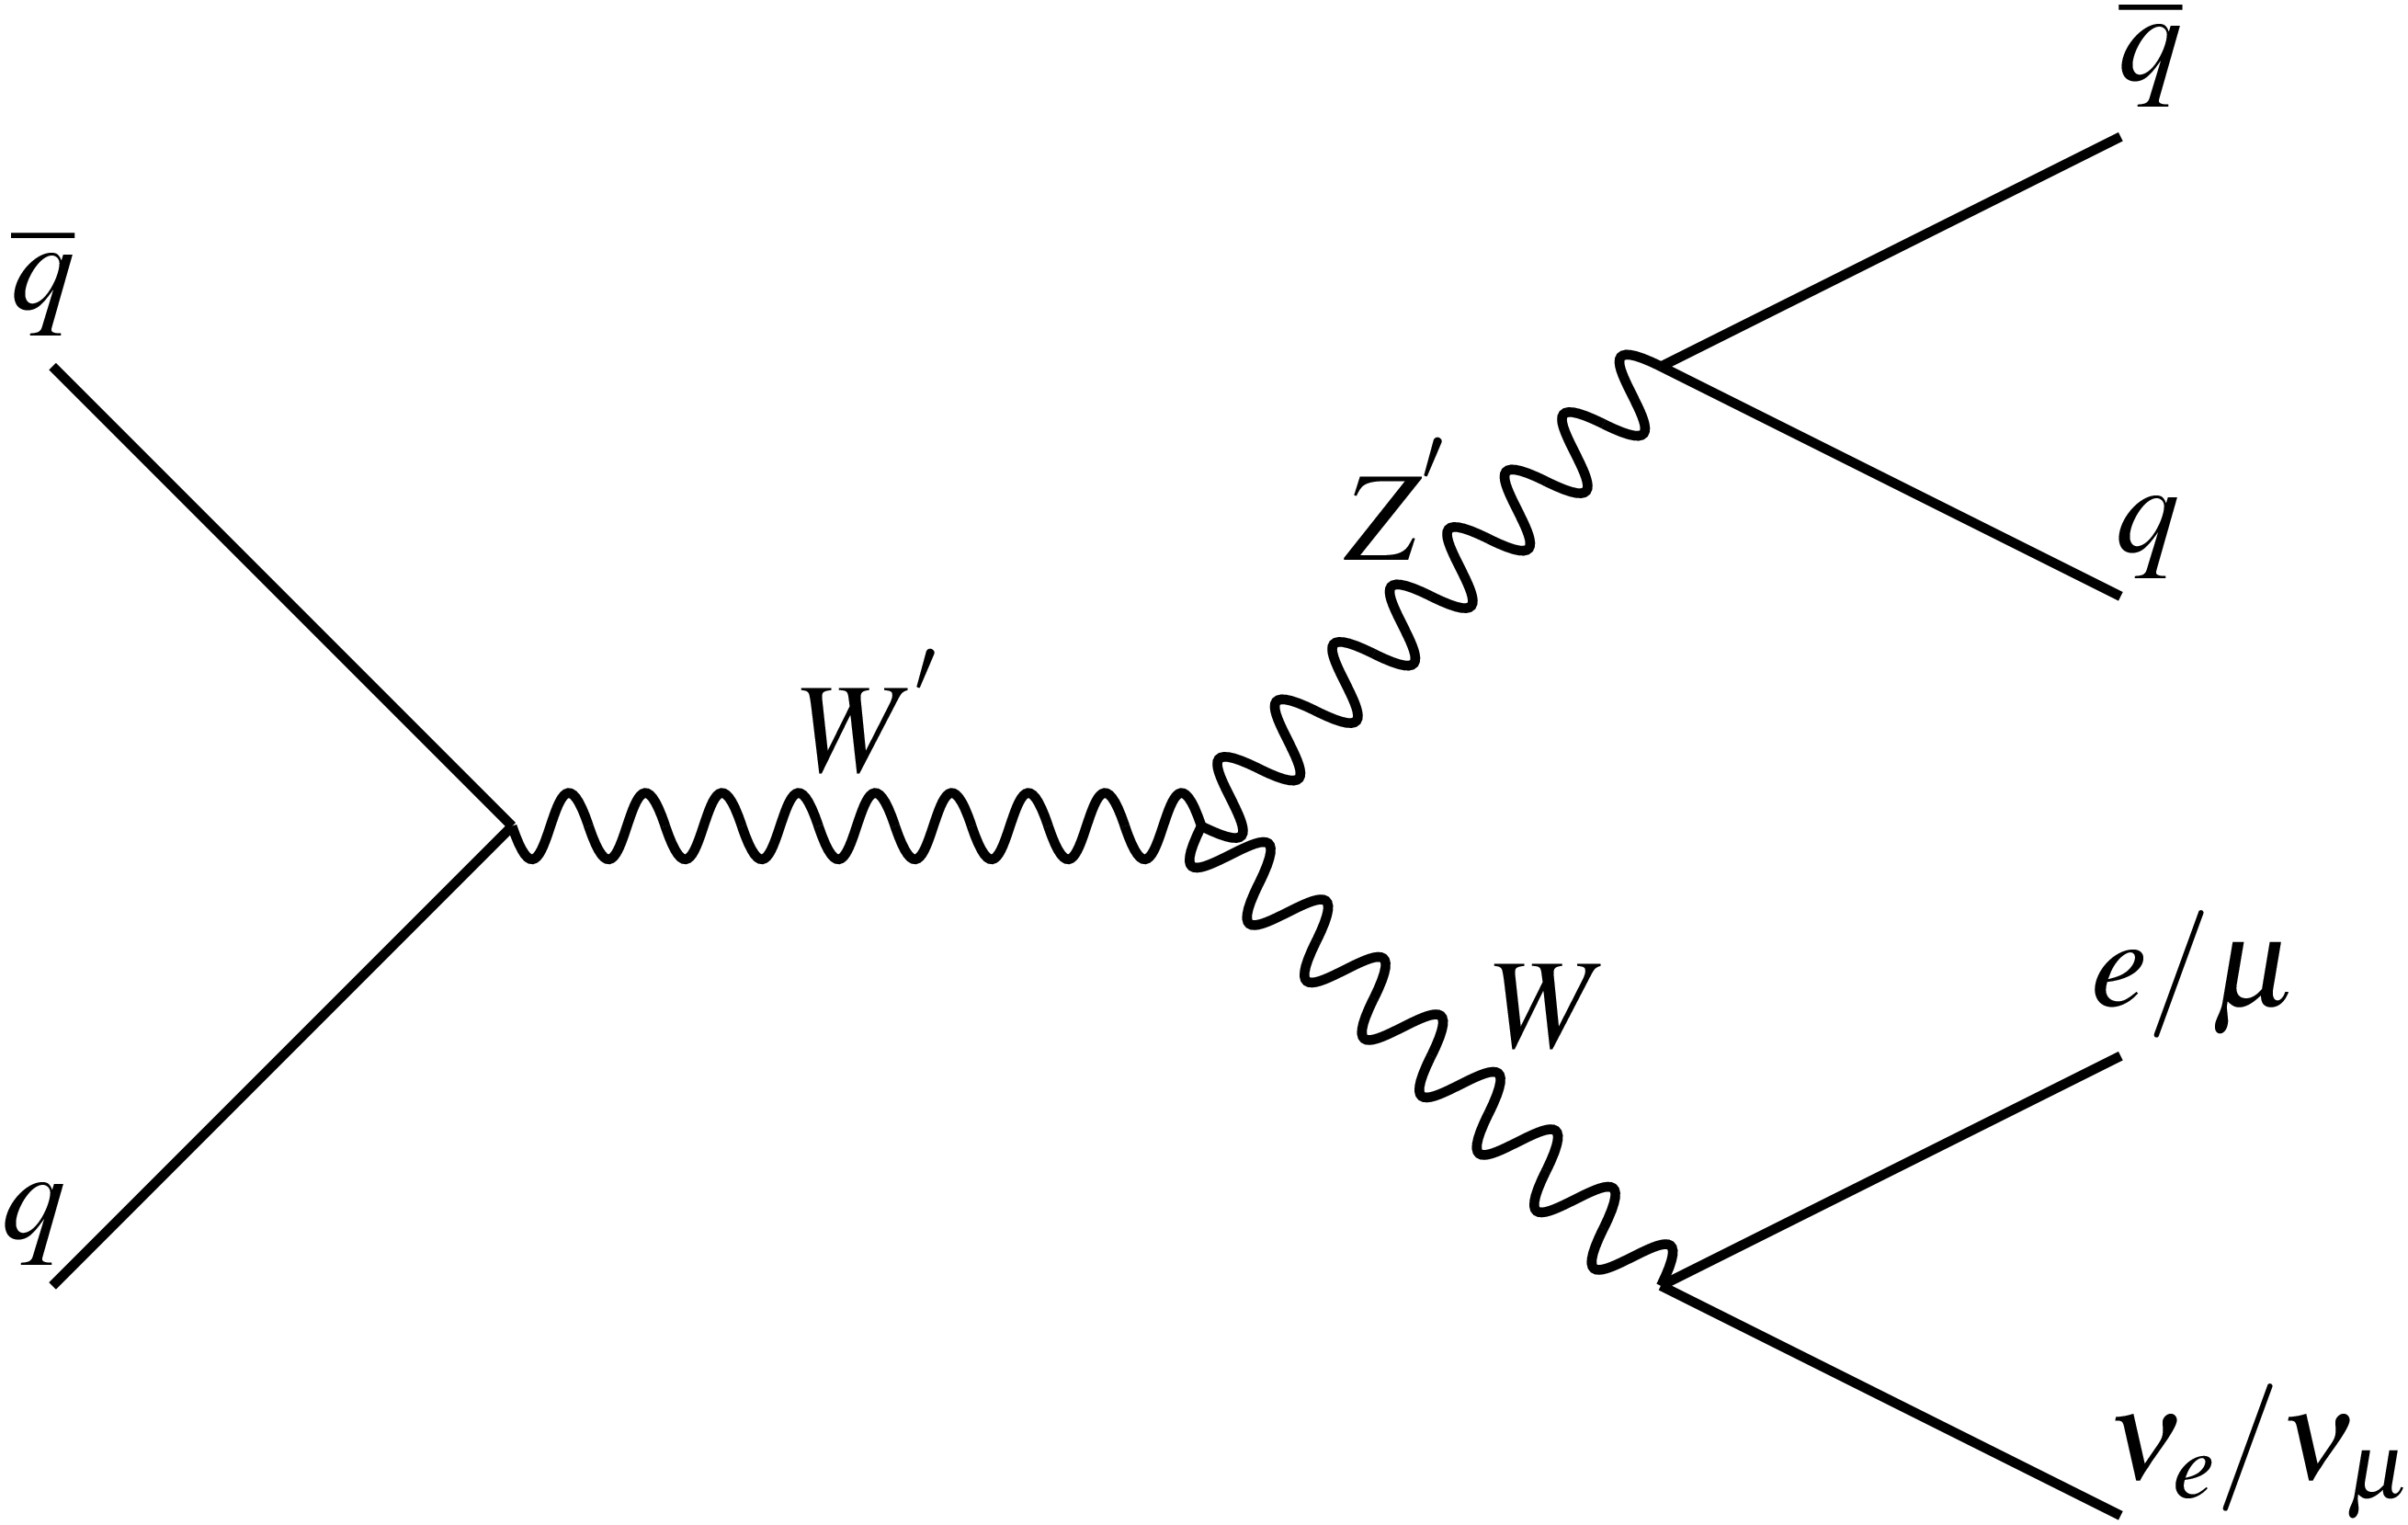
\includegraphics[scale=0.06]{figs/ch6/feynman/fig_01a.png}%
    \caption{Sequential Standard Model}
    \end{subfigure}
    \hfill
    \begin{subfigure}[h]{0.4\linewidth}
    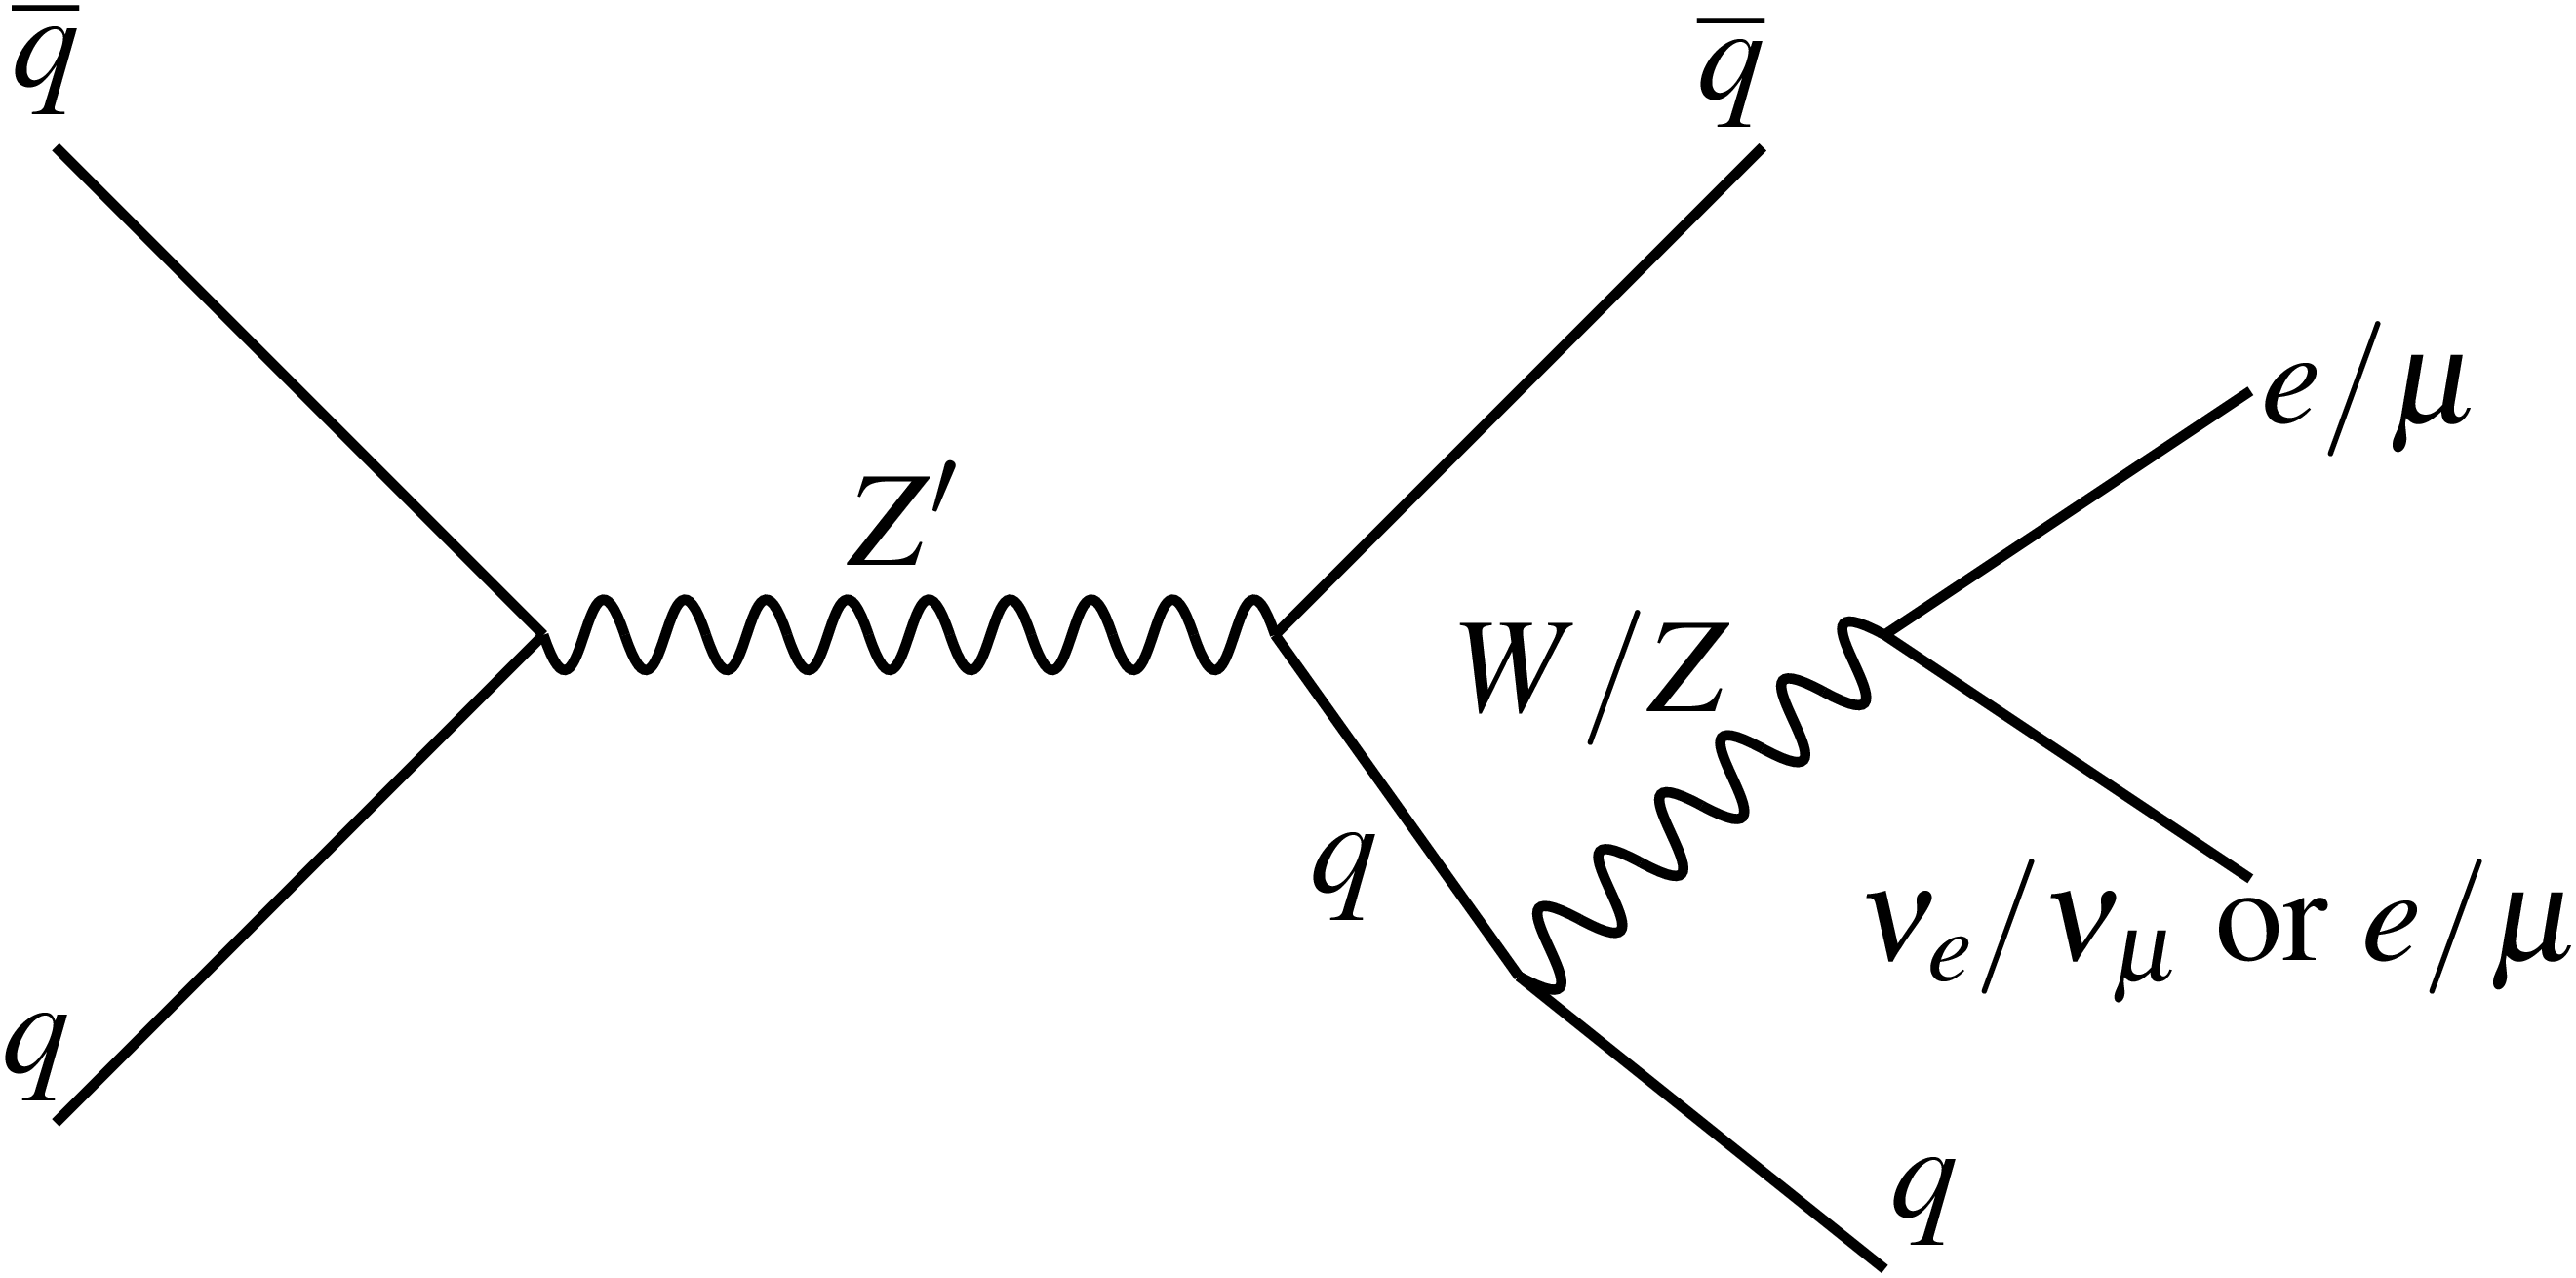
\includegraphics[scale=0.06]{figs/ch6/feynman/fig_01b.png}%
    \caption{Simplified DM Model}
    \end{subfigure}
    \hfill
    \begin{subfigure}[h]{0.4\linewidth}
    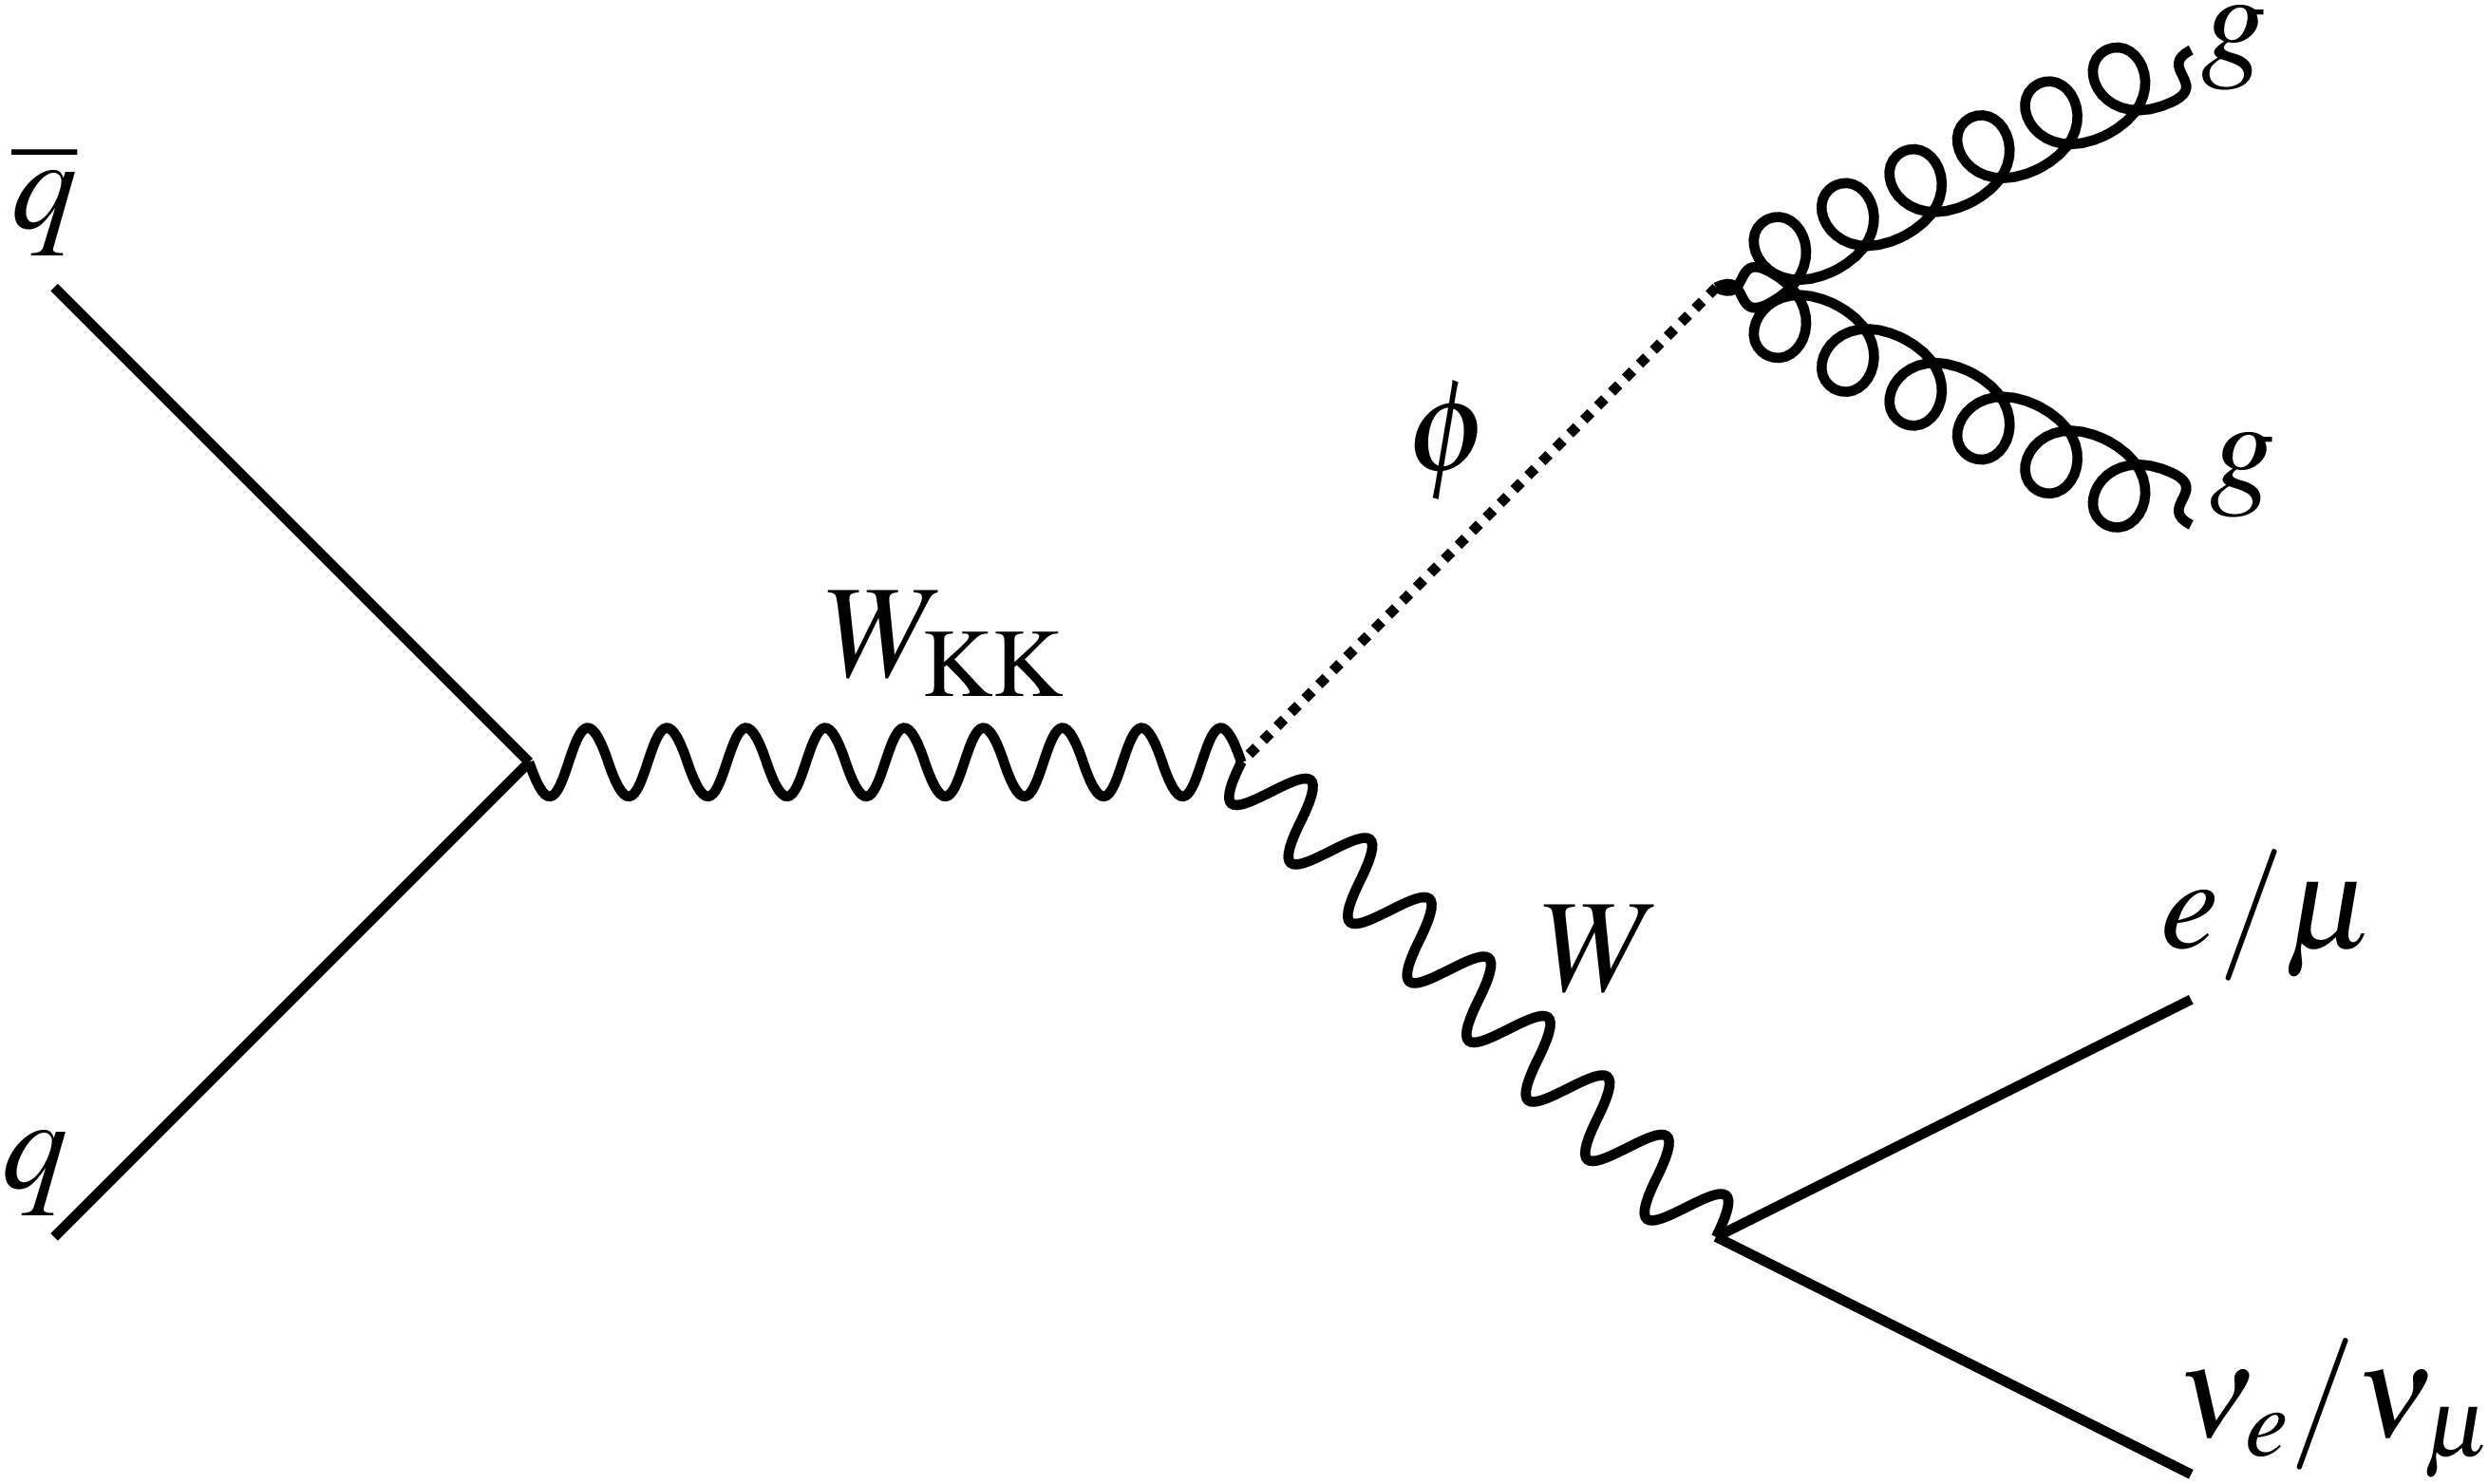
\includegraphics[scale=0.06]{figs/ch6/feynman/fig_01c.png}%
    \caption{Radion Model}
    \end{subfigure}
    \hfill
    \begin{subfigure}[h]{0.4\linewidth}
    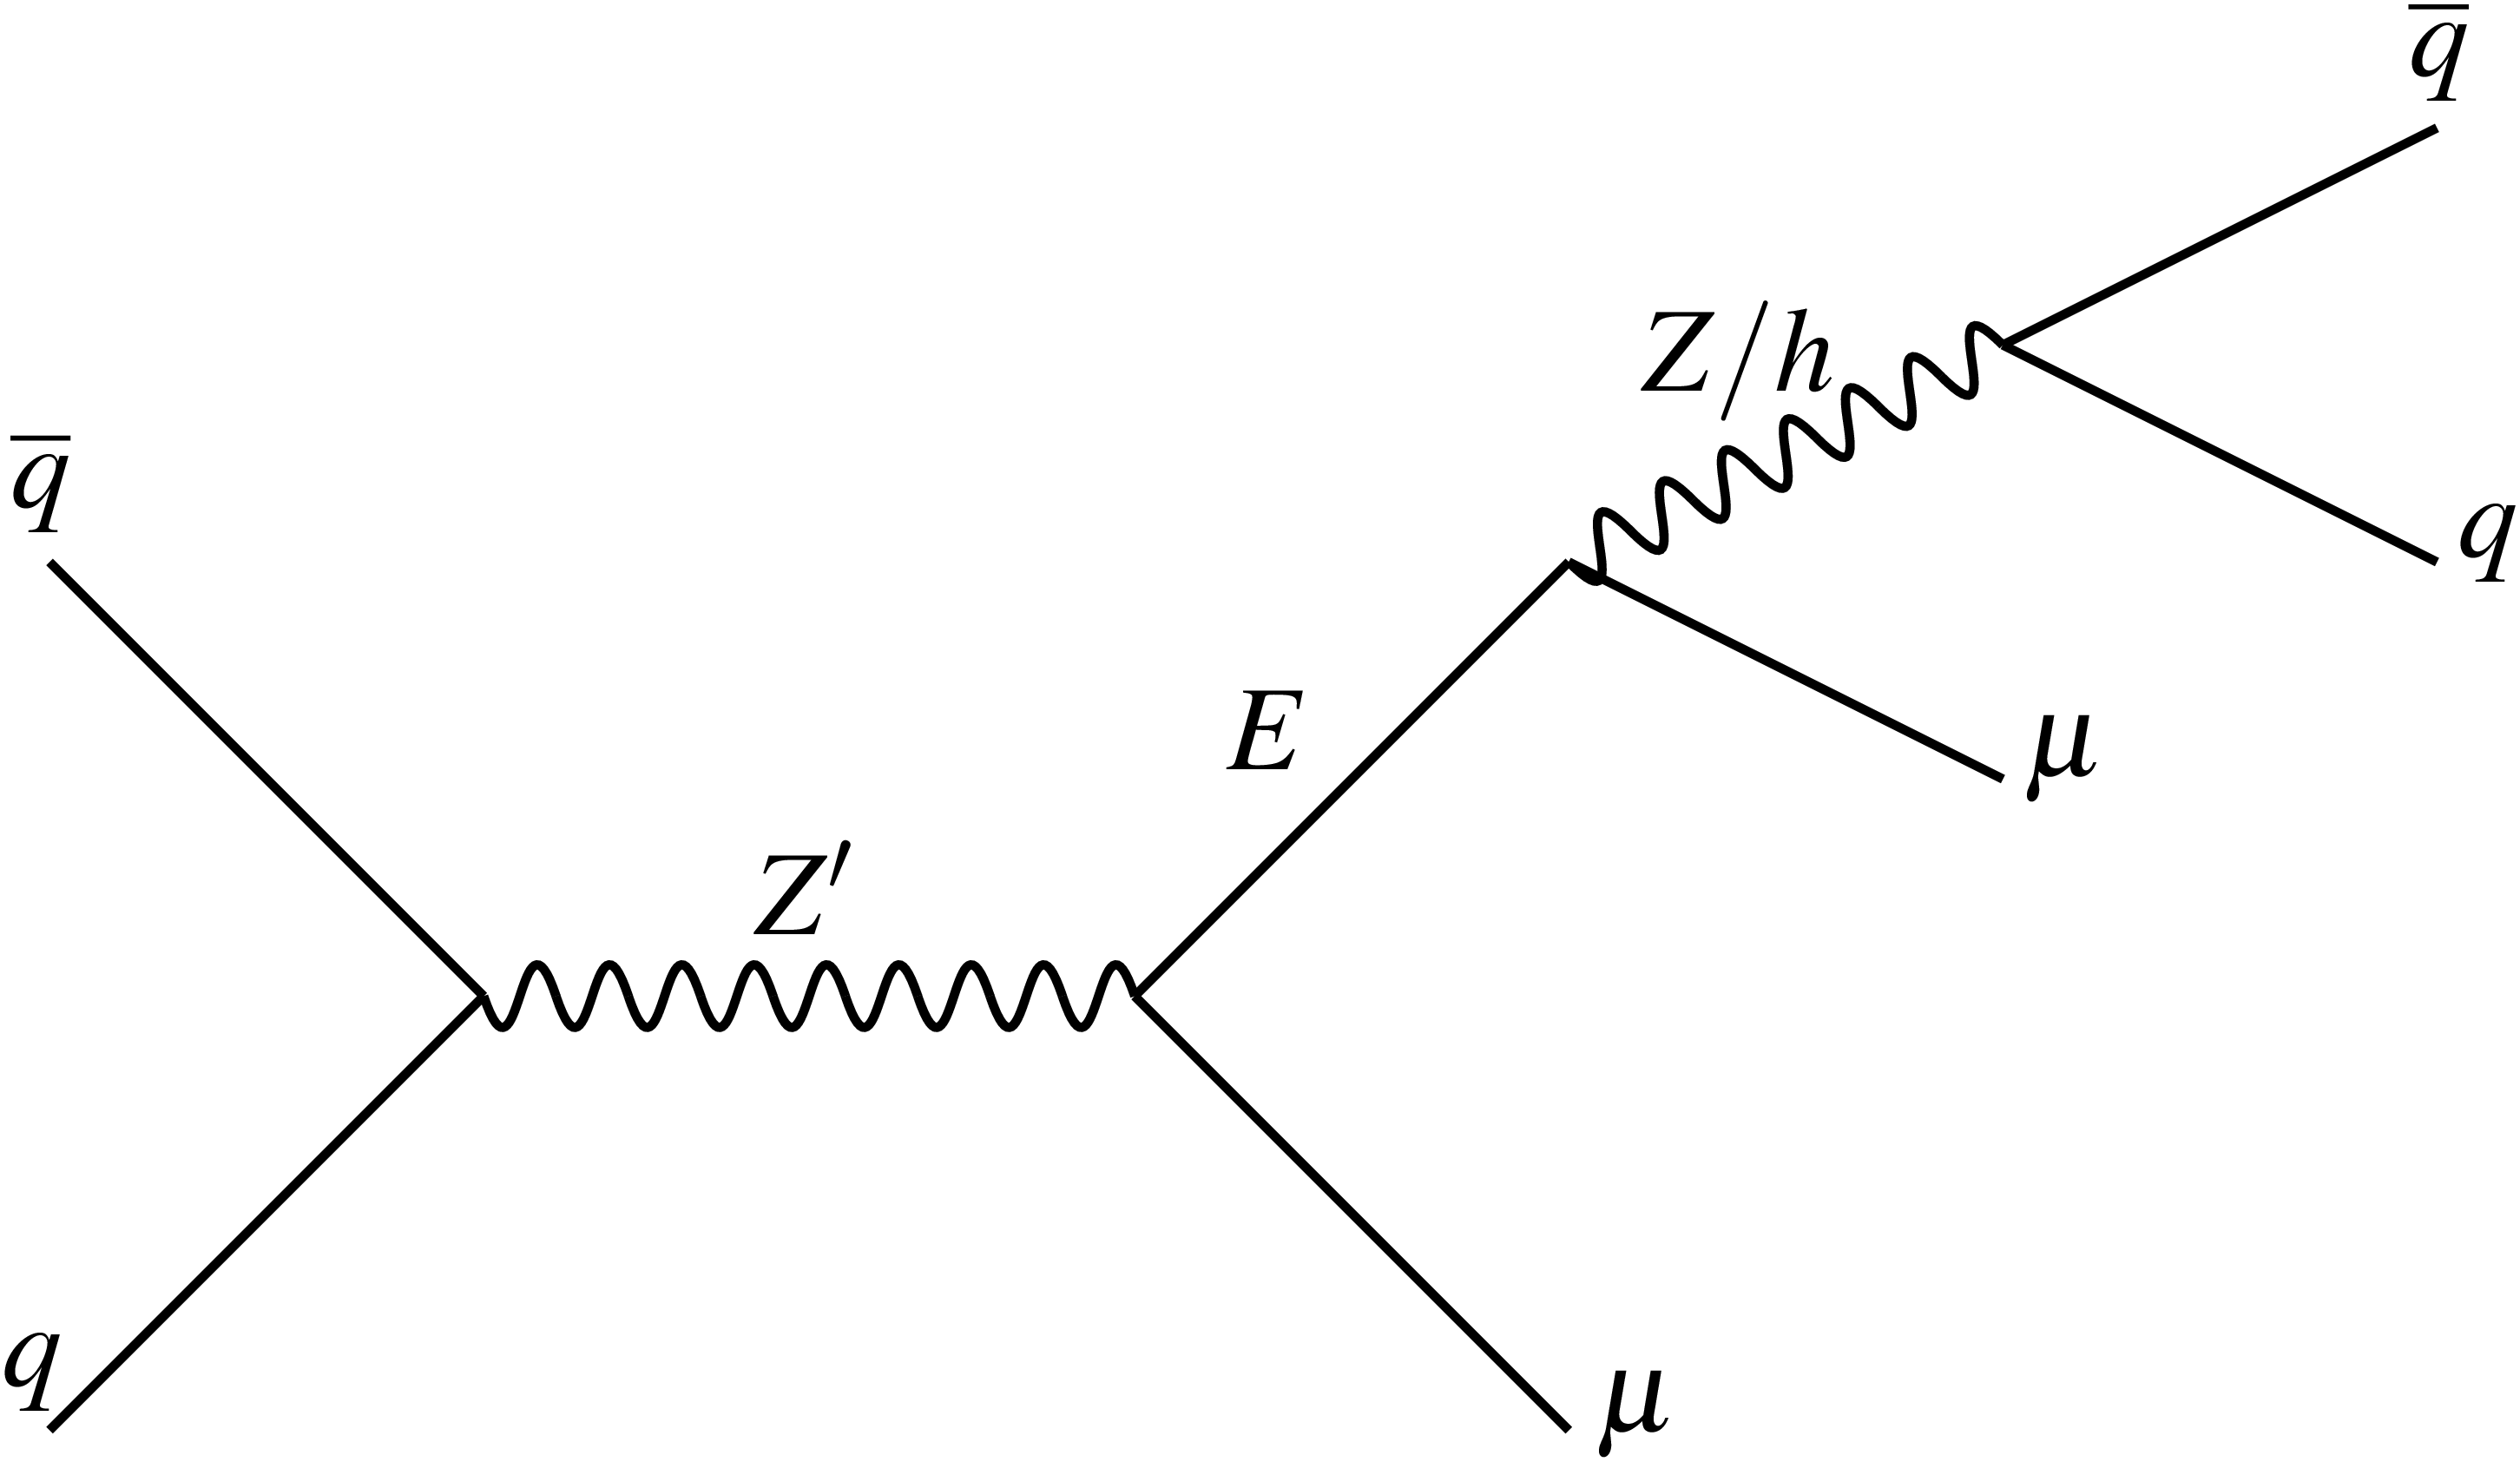
\includegraphics[scale=0.06]{figs/ch6/feynman/fig_01d.png}%
    \caption{Composite-lepton Model}
    \end{subfigure}
    \hfill
    \begin{subfigure}[h]{0.4\linewidth}
    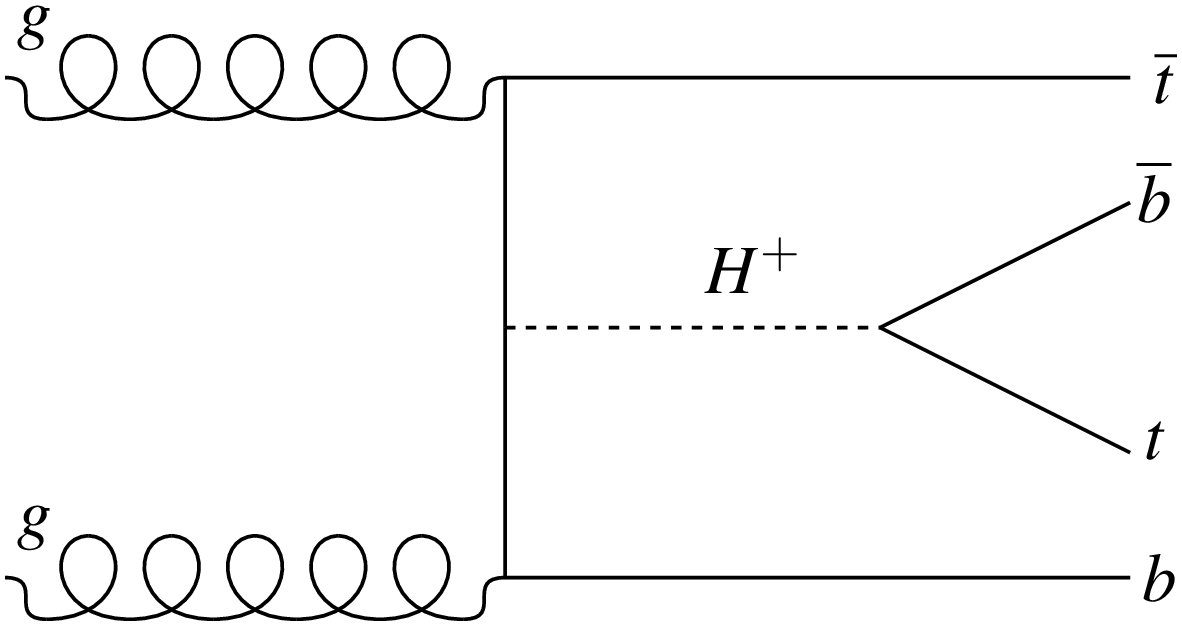
\includegraphics[scale=0.16]{figs/ch6/feynman/fig_01e.png}%
    \caption{Charged Higgs Model}
    \end{subfigure}
    \hfill
    \caption{ Feynman diagrams of the benchmark BSM models.}
\label{fig:bsm-feynman}
\end{figure}

\subsection{Sequential Standard Model}

The Sequential Standard Model (\gls{ssm}) is an extended gauge model~\cite{ssm} which proposes heavy gauge bosons which are commonly denoted as $\textrm{W}'$ and $\textrm{Z}'$. 
The emission of a $\textrm{W}$ boson was considered from the s-channel production

\begin{equation}\label{eq:6.1}
	qq \rightarrow \textrm{W}' \rightarrow \textrm{W Z}' \rightarrow (\textrm{l}\nu)(\textrm{qq})
\tag{6.1}
\end{equation}

where $\textrm{Z}'$ is a new dijet resonance that is produced in association of the W boson~\cite{Zp}. The branching ratio $\textrm{W}'$ to $\textrm{Z}'\textrm{W}$ was set to 50\%, 
while 100\% branching from $Z\to jj$ was set to increase the efficiency of \gls{mc} production. 

\subsection{Simplified Dark Matter Model}

The simplified dark matter (\gls{dm}) models contain one or more stable, long-lived \gls{dm} particle along with an unstable mediator particle that interacts between \gls{dm} and 
the \gls{sm}. The model used in this analysis consists of a single spin-1 mediator denoted as $\textrm{Z}'$ created through a new U(1) gauge symmetry. The final states contain 
one or more leptons/

\subsection{Kaluza-Klein Bosons Decaying to Radions}

In order to solve the elector-weak hierarchy problem and flavor structure origin, some \gls{bsm} theories predict warped higher dimensional compactifications with bulk \gls{sm}. 
In the model used for this analysis, a Kaluza-Klein (\gls{kk}) excitation gauge boson may decay into a particle called the radion and a \gls{sm} gauge boson~\cite{wkk1,wkk2}. 

\begin{equation}\label{eq:6.2}
\textrm{Wkk} \to \textrm{W} + \varphi \to \textrm{l}\nu + \textrm{gg}  
\tag{6.2}
\end{equation}

where $\textrm{Wkk}$ denotes the \gls{kk} boson and the $\varphi$ is a radion decaying into two gluons. 

\subsection{Composite-Lepton Model}

Composite resonances breaking lepton flavor universality predicts a $\textrm{Z}'$ particle that decays into a composite lepton (\textit{E}) and a \gls{sm} lepton~\cite{comp-lep}. The 
composite lepton then decays into a lepton and a Higgs boson or Z boson. 

\begin{equation}\label{eq:6.3}
\textrm{Z}' \to \textrm{l} + \textrm{E}; \textrm{E} \to \textrm{e} + \textrm{Z/h}; \textrm{Z/h} \to \textrm{q}\bar{\textrm{q}}
\tag{6.3}
\end{equation}

\subsection{Charged Higgs Model}

Many \gls{bsm} models predict the existence of a charged Higgs boson. For this analysis, the simulated process assumes the charged Higgs boson is produced along with a top quark and 
a bottom quark~\cite{ch-higg1}. It then decays itself into a top and bottom quark. In the very boosted regime, such as $\textrm{H}^{+}$ masses above 1 TeV, a b-jet and a jet originated from a top quark 
form almost back-to-back, which would be reconstructed via the $\textrm{m}_{\textrm{jj}}$ distributions. For lower, non-boosted masses, the leading and non-leading jets lead to 
an approximate invariant mass of the $\textrm{H}^{+}$ and end in a rather broad resonance due to incomplete reconstruction of the decay products. 

\section{Event Input Representation}\label{sec:evnt-input-rep}

Now that the pre-selection has been chosen, the question is how to represent this as input for a machine learning model in order to maximize underlying 
correlations and pattern recognition. The overall goal of this analysis is to find anomalous dijet resonances, but the input must ensure that the model is not biased towards 
only kinematic anomalies. The approach that was taken for this analysis was to represent the input as a matrix that contains correlations between each object within the event.
This matrix is called the Rapidity Mass Matrix, or \gls{rmm}. Figure \ref{fig:rmm} shows an example of the \gls{rmm} with two object types, jets (\textit{j}) and muons (\textit{μ}). The 
maximum amount of objects is set to \textit{N}. The position (1,1) contains the event's missing transverse energy, or \gls{met}, and is scaled by the center of mass energy (1/$\sqrt{\textrm{s}}$)
where $\sqrt{\textrm{s}}$ is the center-of-mass energy. The diagonal cells contain the ratio $e_T(i_n)$ = $\textrm{E}_{\textrm{T}}(\textrm{\textit{i}}_{\textrm{1}})$/$\sqrt{\textrm{s}}$,
where $\textrm{E}_{\textrm{T}}(\textrm{\textit{i}}_{\textrm{1}})$ is the transverse energy of a leading object \textit{i} (a jet or \textit{μ}), and transverse energy imbalances

\begin{equation}\label{eq:6.4}
\delta e_T(i_n) = \frac{E_T(i_{n-1})-E_T(i_{n})}{E_T(i_{n-1})+E_T(i_{n})}, \quad n=2,\ldots, N,  
\tag{6.4}
\end{equation}

for a given object type \textit{i}. All objects are strictly order in transverse energy, i.e. $\textrm{E}_T(i_{n-1})>\textrm{E}_T(i_{n})$. The top row are the particle's transverse masses $\textrm{M}_T(i_n)$
for two-body decays, scaled by 1/$\sqrt{s}$, i.e.  $\textrm{m}_T(i_n)=\textrm{M}_T(i_n)/\sqrt{s}$.
The upper-right quadrant shown in red are the non-diagonal values of $\textrm{\textit{m}}(i_n,j_k)=\textrm{M}_{i,n,\> j,k}/\sqrt{s}$, where $\textrm{M}_{i,n,\> j,k}$ are two-particle invariant masses. 
The first column vector s $h_L(i_n) = C (\textrm{cosh}(y)-1)$, where $y$ is the rapidity of a particle $i_n$, and $C$ is a constant defined such that the average 
values of $h_L(i_n)$ can correspond to certain algorithms that may require values to have similar weights. The values in the bottom-left quadrant highlighted in green $h(i_n,j_k)=C( \textrm{cosh}(\Delta \textrm{y} / \textrm{2}  )-\textrm{1} )$ 
are constructed from the rapidity differences $\Delta y=y_{i_k} - y_{j_n}$ between \textit{i} and \textit{j}.

\begin{figure}[ht]
    \centering
    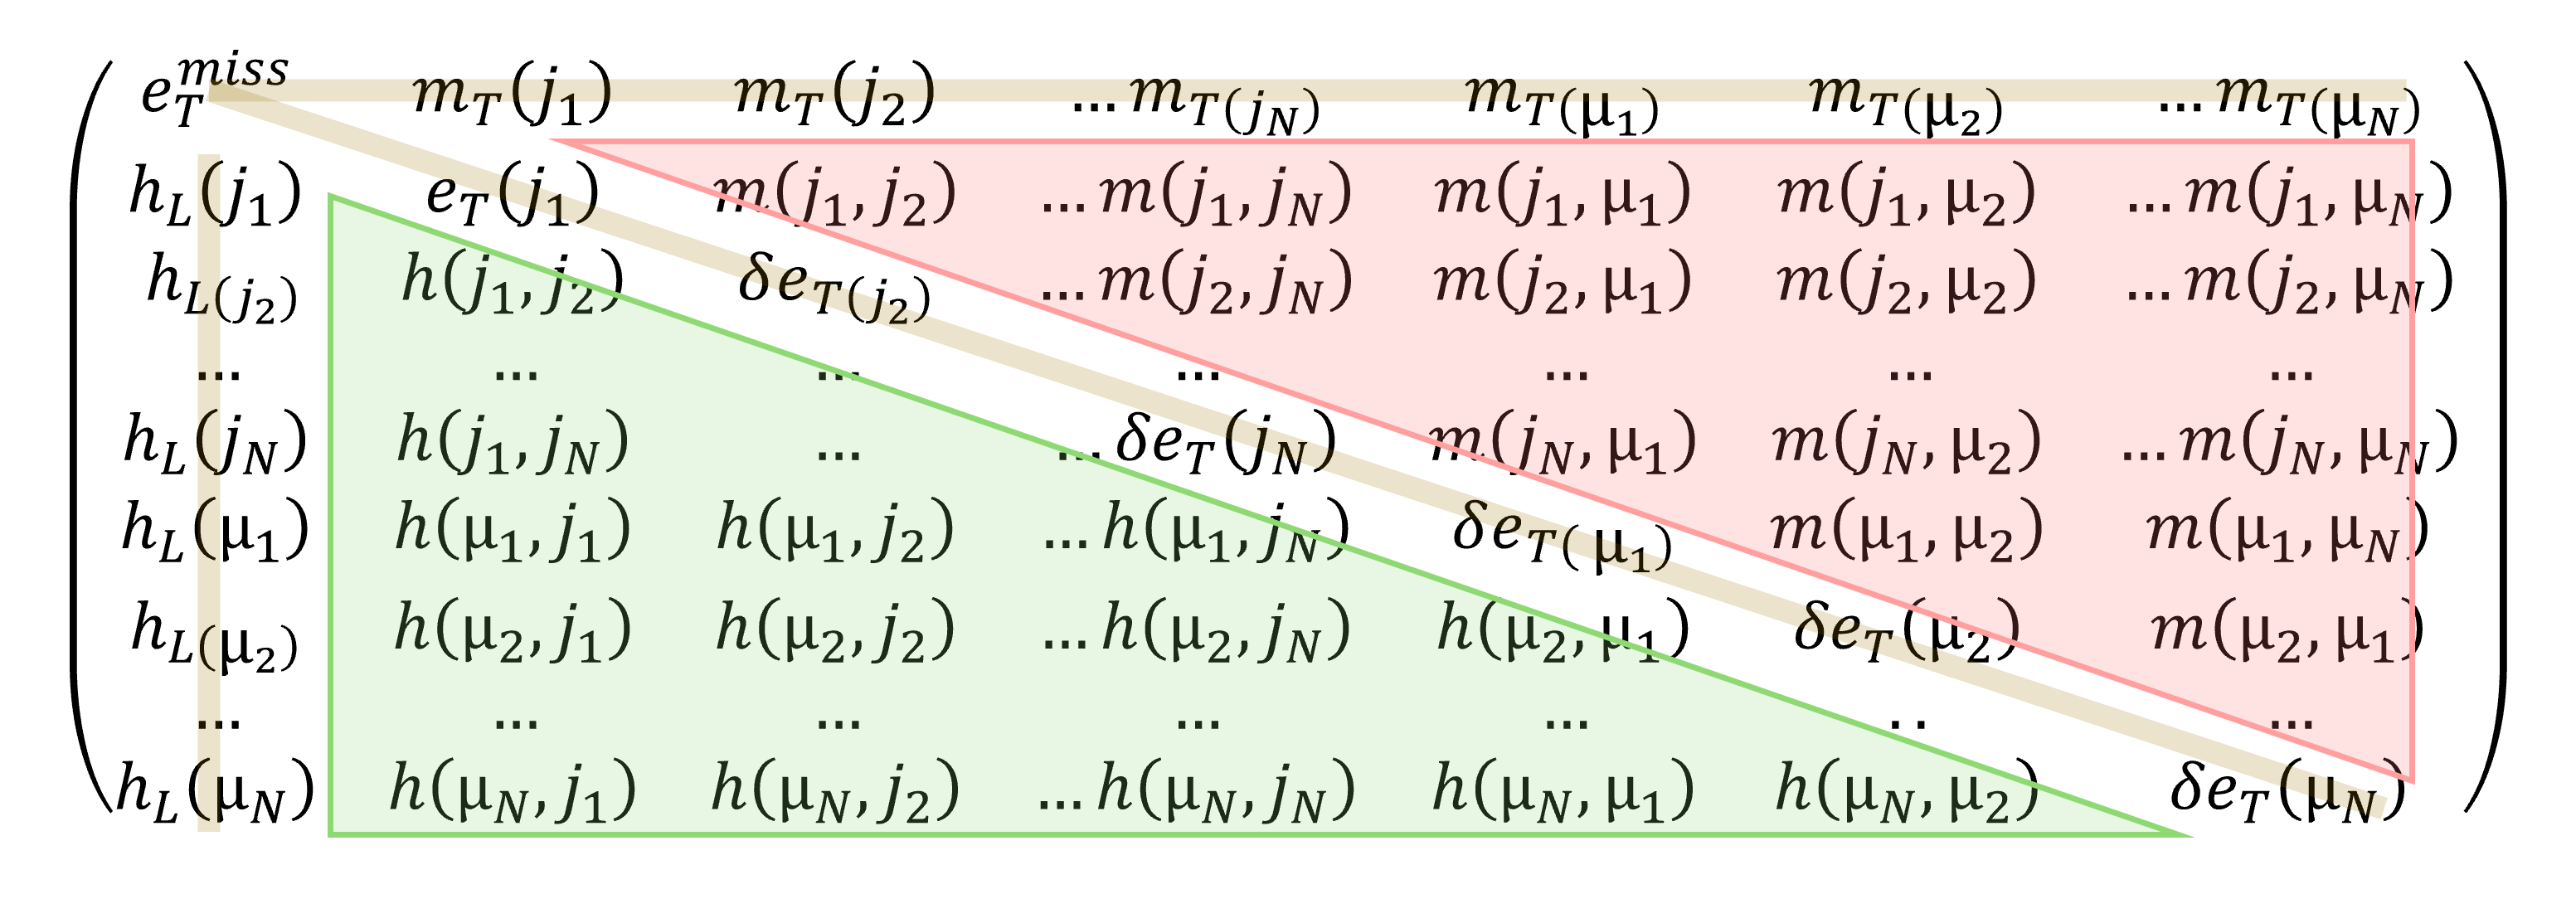
\includegraphics[scale=0.68]{figs/ch6/rmm/RMM.png}
    \caption{ Example of the Rapidity Mass Matrix using only two objects, jets (\textit{j}) and muons (\textit{μ}).}
\label{fig:rmm}
\end{figure}

Applying this idea to this analysis expounds this example \gls{rmm} into a larger representation. In the end, nine invariant masses were studied, therefore the \gls{rmm} had to contain all the objects that were 
used in combination for the invariant masses. The total objects per event varies event to event. In order to deal with this variable sizing, the events were ``mapped'' to a fixed data-structure and therefore 
implement zero-padding for missing data. The the standard topology of reconstructed objects was used while setting a maximum number for each object. In total, up to 10 jets, 10 b-jets, 5 electrons, 5 muons, 
5 photons and \gls{met} were allowed (total of 36 objects). In order to reduce biasing the \gls{ml} model on the di-object invariant masses of interest, the values that correspond these nine invariant masses are zero-padded 
for every event. This gives us a total amount of variables to feed the model of 1287 ($\textrm{36}^{\textrm{2}}$-9=1287). Figure~\ref{fig:zero-rmm} shows an example \gls{rmm} with all indices allotted for objects to be filled and 
shown as yellow, whereas the zero-padded indices are shown in blue. The indices corresponding to the nine invariant masses of interest are removed to reduce bias. Appendix shows examples of single events converted to \gls{rmm}s.

\begin{figure}[H]
    \centering
    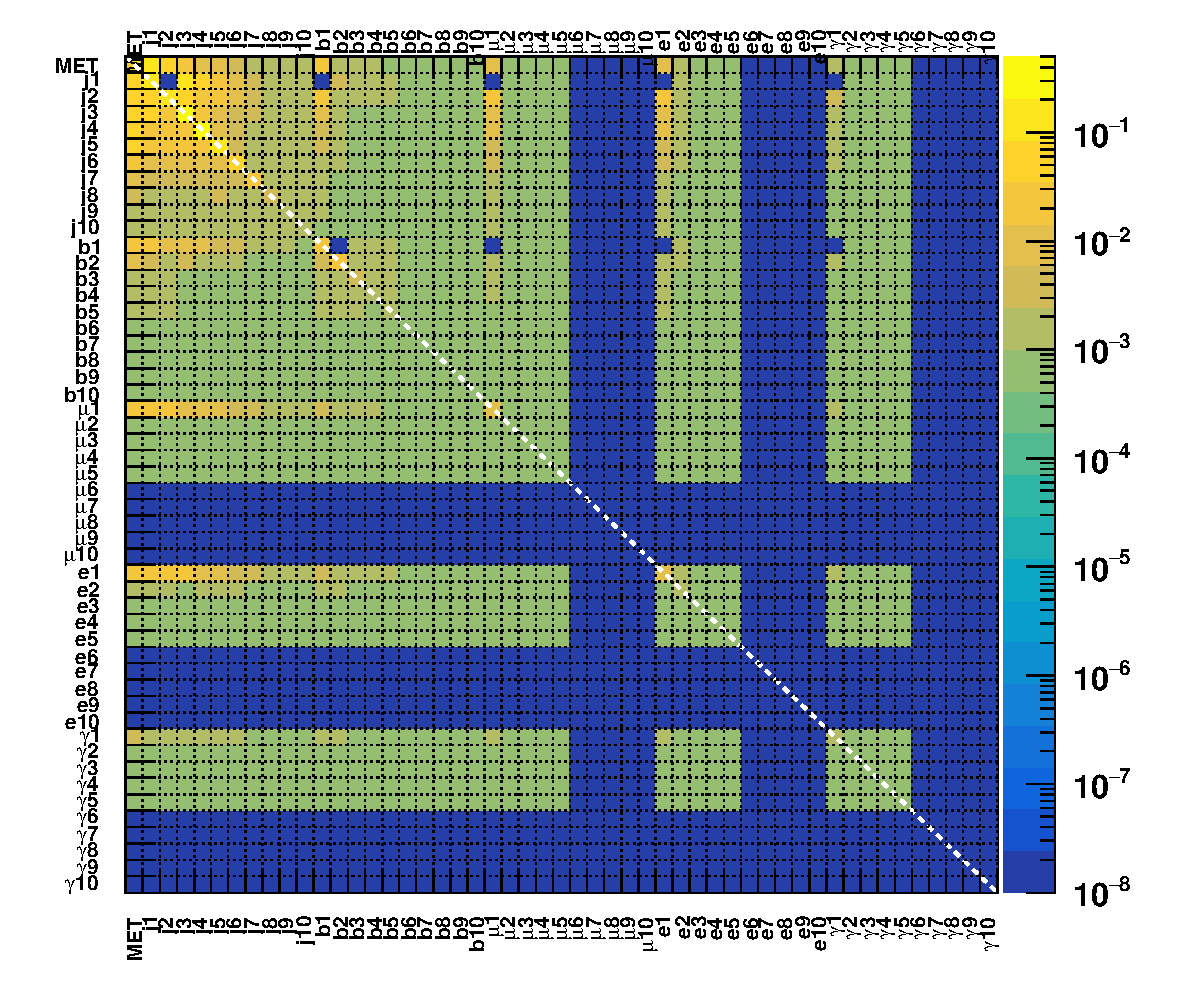
\includegraphics[scale=0.82]{figs/ch6/rmm/make_0removal.pdf}
    \caption{ This RMM diagram shows the indices that allow values (yellow) and the zero-padded indices (blue). The nine invariant masses of interest are removed (blue). This diagram shows the average values of cells for 10000 events. The total of non-zero variables is 1287.}
\label{fig:zero-rmm}
\end{figure}

\section{Autoencoder Training}\label{sec:ae-training}

The \gls{ae} model was trained using \texttt{TensorFlow} \cite{tensorflow} with a Keras backend \cite{keras}. The \gls{ae} architecture is a deep-learning algorithm that is used
for high-dimensionality reconstruction. The architecture is split into three parts. The first part is called the ``encoder'' which is the initial compression neurons which compresses 
the input into lower dimensionality. The second part of this architecture is referred to as the ``latent layer'' and is considered the bottleneck. This is a single layer of neurons
that holds the compressed input. The final stage of this architecture is called the ``decoder'' which decompresses the latent layer in order to reconstruct the original input. The 
neural-network of the decoder typically mirrors that of the encoder. The chosen amount of neurons should for these layers are optimized for the goal of anomaly detection.
\par
The \gls{ae}s purpose is to reconstruct its input. When the input gets compressed and then decompressed by the \gls{ae}, there is a certain amount of data lost within the process. 
This value is determined by the loss function that the model is trained to minimize. The loss function used for this model is the mean squared error function (\gls{mse}) which can be 
seen in Eq.~\ref{eq:6.5}

\begin{equation}\label{eq:6.5}
    \textrm{\textit{Loss}} = \frac{1}{\textrm{\textit{n}}} \sum_{i=1}^{n=1287} (\textrm{\textit{x}}_{\textrm{\textit{i}}}-\hat{x}_{\textrm{\textit{i}}})^{\textrm{2}}
\tag{6.5}
\end{equation}

It is known for \gls{ae}s that it's possible to have exactly zero loss when decompressing the input. This zero loss is not the goal of this architecture for the value of the loss is chosen to be the score in 
which indicates anomalous events. Therefore, the optimized architecture must have a range of loss values while maximizing the separation between \gls{sm} events and \gls{bsm} events.  The architecture topology 
studies for this optimization can be found in Appendix~\ref{appendix:ae-topo-studies}. The resulting optimized architecture chosen is seen in Table~\ref{tab:ae-arch}. The total number of trainable weights is 2,863,087,
the activation function used is the ``leakyReLU'' and the loss function is minimized by the Adam Optimizer. The reconstruction loss is used as the anomaly score. 

\begin{table}[H]
    \begin{verbatim}
        _________________________________________________________________
        Layer (type)                 Output Shape              Param #
        =================================================================
        input_1 (InputLayer)         [(None, 1287)]            0
        _________________________________________________________________
        dense (Dense)                (None, 800)               1030400
        _________________________________________________________________
        dense_1 (Dense)              (None, 400)               320400
        _________________________________________________________________
        dense_2 (Dense)              (None, 200)               80200
        _________________________________________________________________
        dense_3 (Dense)              (None, 400)               80400
        _________________________________________________________________
        dense_4 (Dense)              (None, 800)               320800
        _________________________________________________________________
        dense_5 (Dense)              (None, 1287)              1030887
        =================================================================
        Total params: 2,863,087
        Trainable params: 2,863,087
        Non-trainable params: 0
        \end{verbatim}
        \caption{Optimized Autoencoder architecture chosen for the anomaly detection analysis. More neurons may have optimized it further but was limited due to computational power.}
        \label{tab:ae-arch}
\end{table}

Figure~\ref{fig:AE-arch} shows a schematic of the nominal \gls{ae} model with a sample input and output.
1\% of \gls{atlas} Run 2 data is randomly selected from different data-taking periods were used for training. 70\% were used for training while 30\% were used for validation. Early stopping was set to 30 epochs. 
\gls{mc} samples nor labels were used for training, thus making this approach a data-driven unsupervised learning. Figure~\ref{fig:training-stats} shows the training loss per epoch for both the training and validation sets. 

\begin{figure}[H]
    \centering
    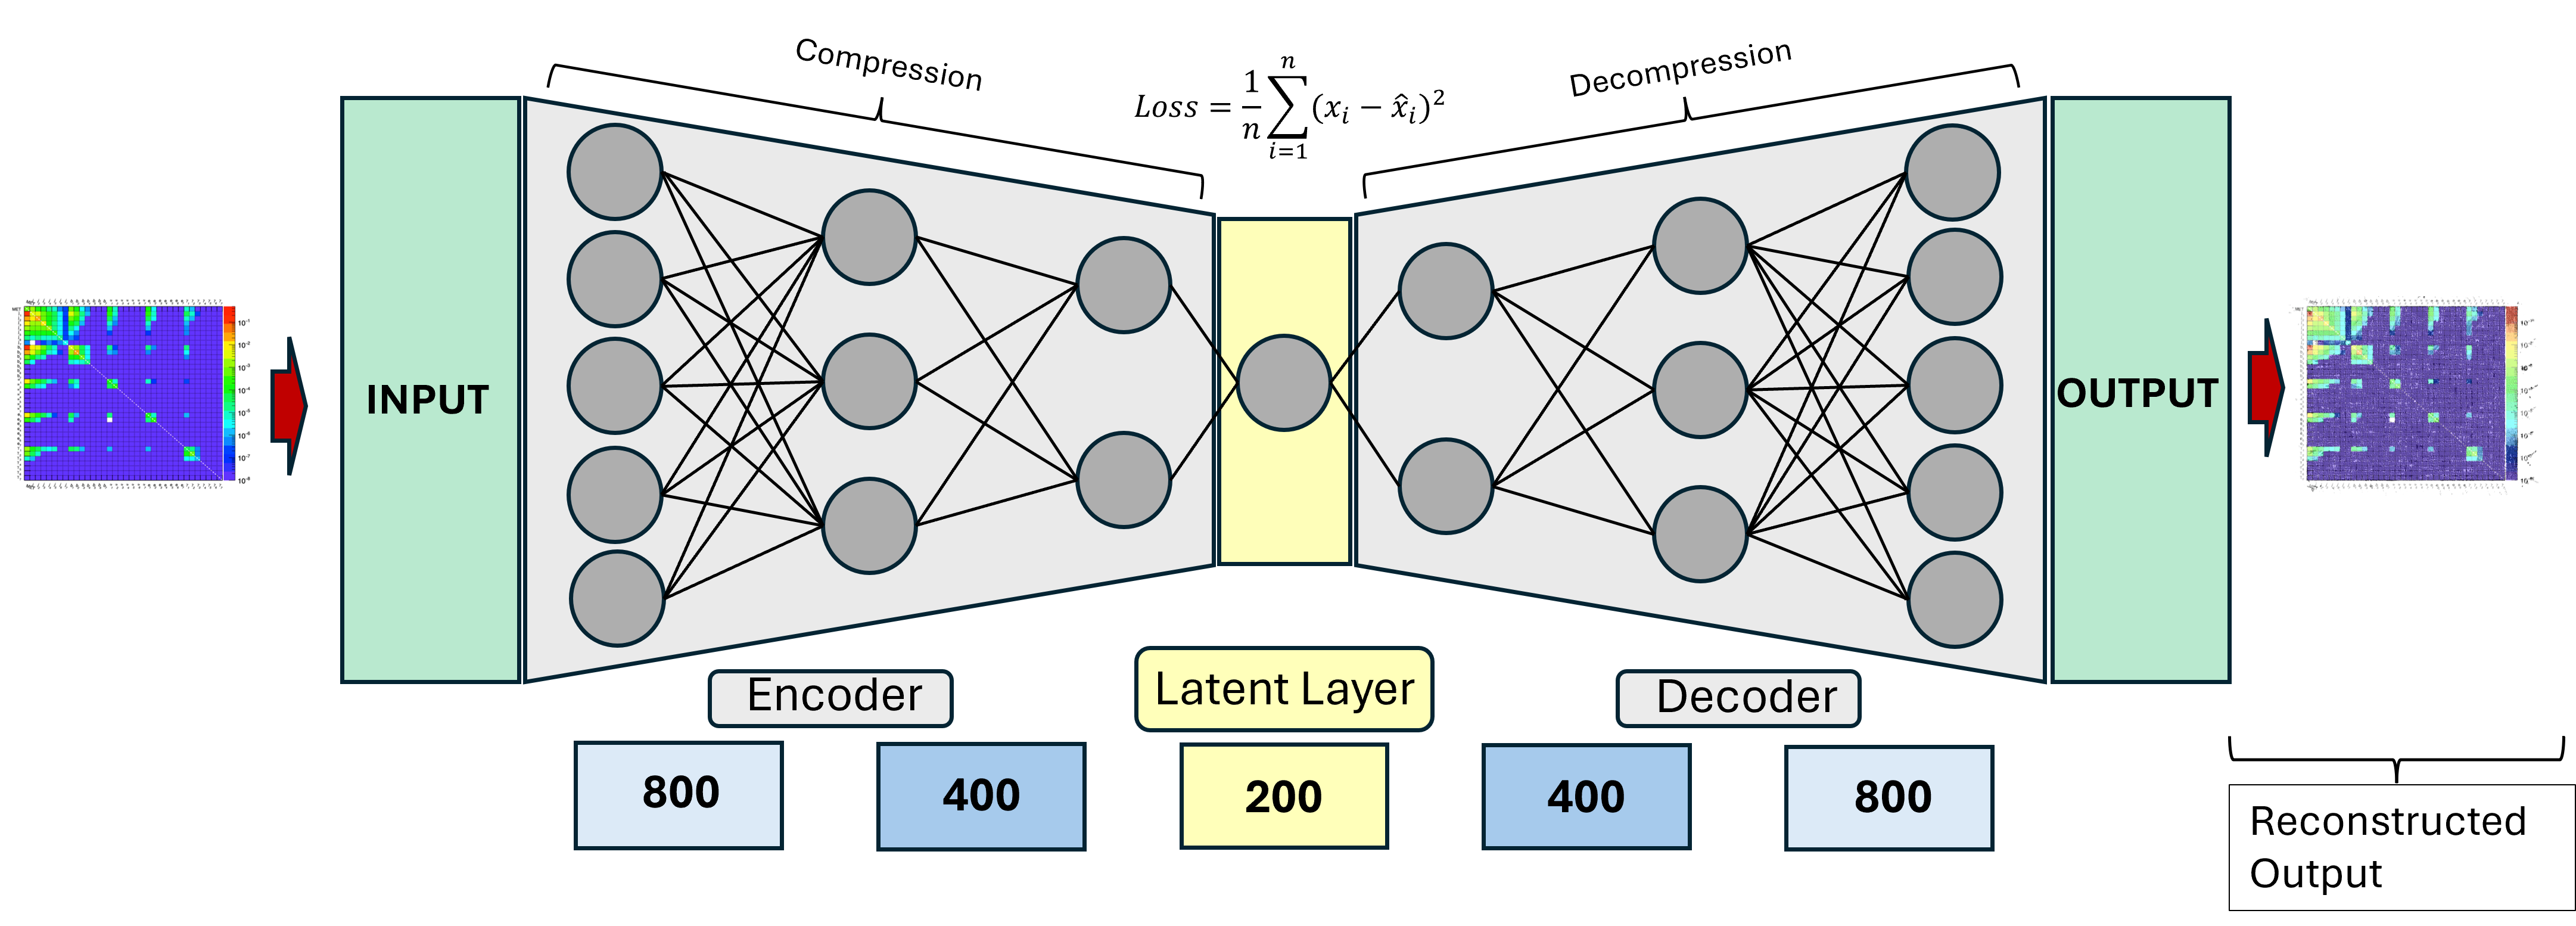
\includegraphics[scale=0.48]{figs/ch6/AE-arch.png}
    \caption{A schematic representation of the nominal AE model with an example input and its output. It's composed of three parts, the encoder which compress the data, the latent layer which acts as the bottleneck
    and the decoder which decompresses the data in order to recreate the original input. Due to this compression and decompression, data is loss via the loss function calculation. This loss is used as the anomaly score.
    When an event that is the model hasn't seen goes through, the data loss is higher and thus can be tagged as anomalous.}
\label{fig:AE-arch}
\end{figure}

\begin{figure}[h]
    \centering
    \begin{subfigure}[h]{0.45\linewidth}
    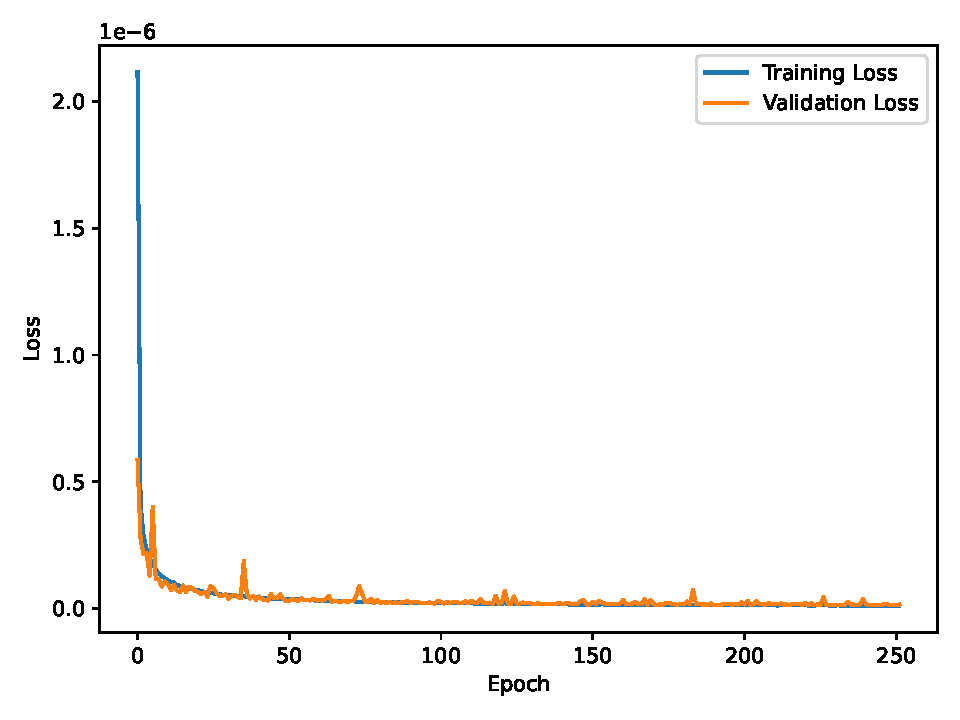
\includegraphics[scale=0.45]{figs/ch6/epoch_vs_loss.pdf}%
    \caption{Loss per epoch (linear)}
    \end{subfigure}
    \hfill
    \begin{subfigure}[h]{0.45\linewidth}
    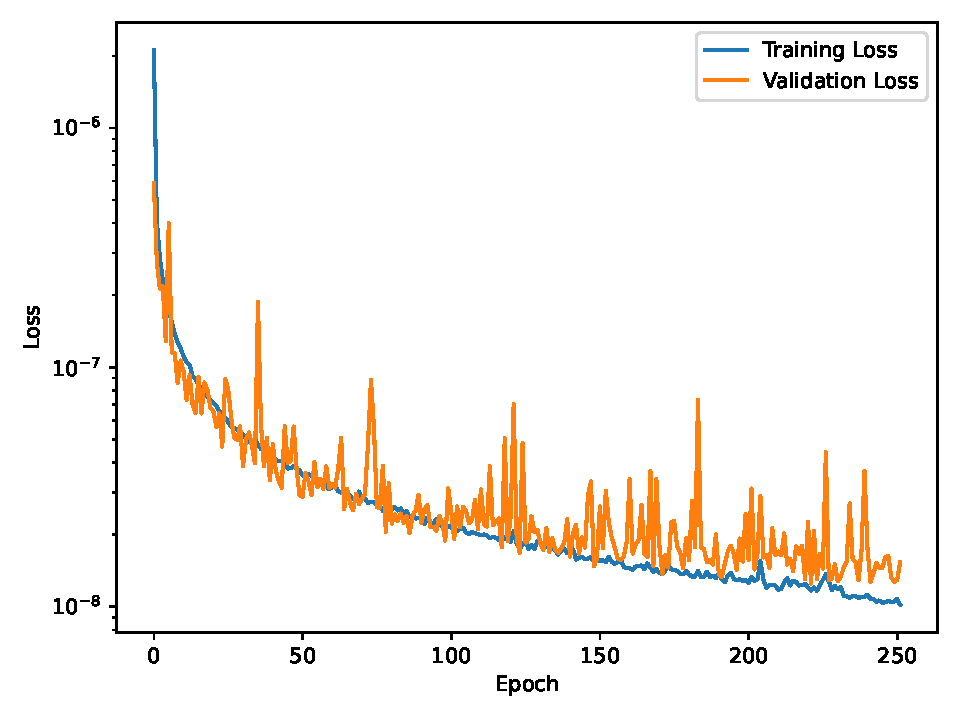
\includegraphics[scale=0.45]{figs/ch6/epoch_vs_loss_log.pdf}%
    \caption{Loss per epoch (log)}
    \end{subfigure}
    \hfill
    \caption{Training and validation loss as a function of epochs shown both linear and log y-scale.}
\label{fig:training-stats}
\end{figure}

Training \gls{ml} models have dependencies on several factors such as random seed values used for \gls{ae} initialization, the processing computer architecture, training/validation dataset splitting, etc.
In order to accommodate for these factors, 50 separate trainings were conducted with different random seed values. Figure~\ref{fig:loss_seed} shows these 50 trainings and the validation value in which the \gls{ae} was stopped training.
The median value of this validation loss is ln(\texttt{loss}) is -10.554. The trained model that stopped at this median value then became the nominal model used for the rest of the analysis. 
The two $\pm$RMS models are used for systematic studies in Appendix~\ref{appendix:ae-systematics}. 

\begin{figure}
    \begin{center}
       \subfloat[Using 1\% of data for training] {
        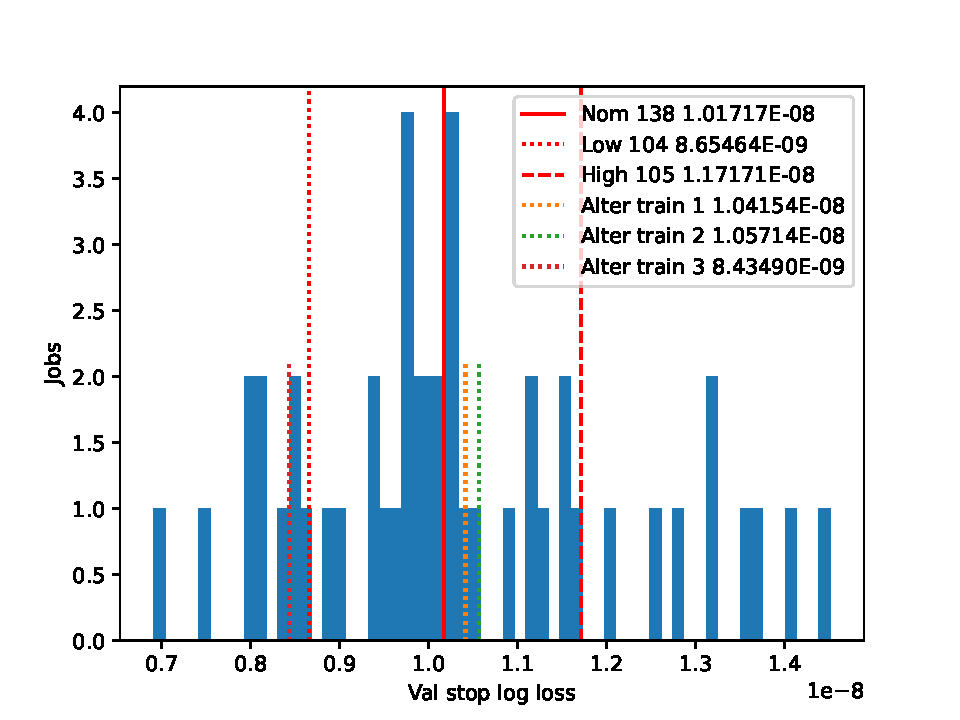
\includegraphics[width=0.8\textwidth]{figs/ch6/seedAEleakyRelu800_400_200_400_800.pdf}
        }
    \end{center}
    \caption{Validation stop loss values for 50 trainings with different seeds. Seed value and corresponding loss value is shown in the legend.
    ``Alter training'' shows different randomly selected training data from full Run 2 ATLAS data. (ROC curves can be found in Appendix~\ref{appendix:ae-systematics})
    Consistent loss values were achieved among different training sets.}
\label{fig:loss_seed}
\end{figure}

The trained nominal \gls{ae} model was used to process \gls{mc} events and \gls{bsm} events and is shown in Figure~\ref{fig:plot_loss_mc}. The ln(\texttt{loss}) value is taken to show anomalous separation.
10\% of randomly chosen data events from Run 2 were used to check the loss distribution 
to ensure that there is good separation between data and \gls{bsm}. It can be seen that in both (a) and (b) in Figure~\ref{fig:plot_loss_mc} that there is good separation between \gls{sm} and \gls{bsm} events. The year 
dependence is also checked since all of Run 2 is taken over several years. Figure~\ref{fig:loss_year} shows that there is no shape dependence on data-taking years.

\begin{figure}[H]
    \begin{center}
       \subfloat[MC for autoencoder trained with 1\% of data] {
       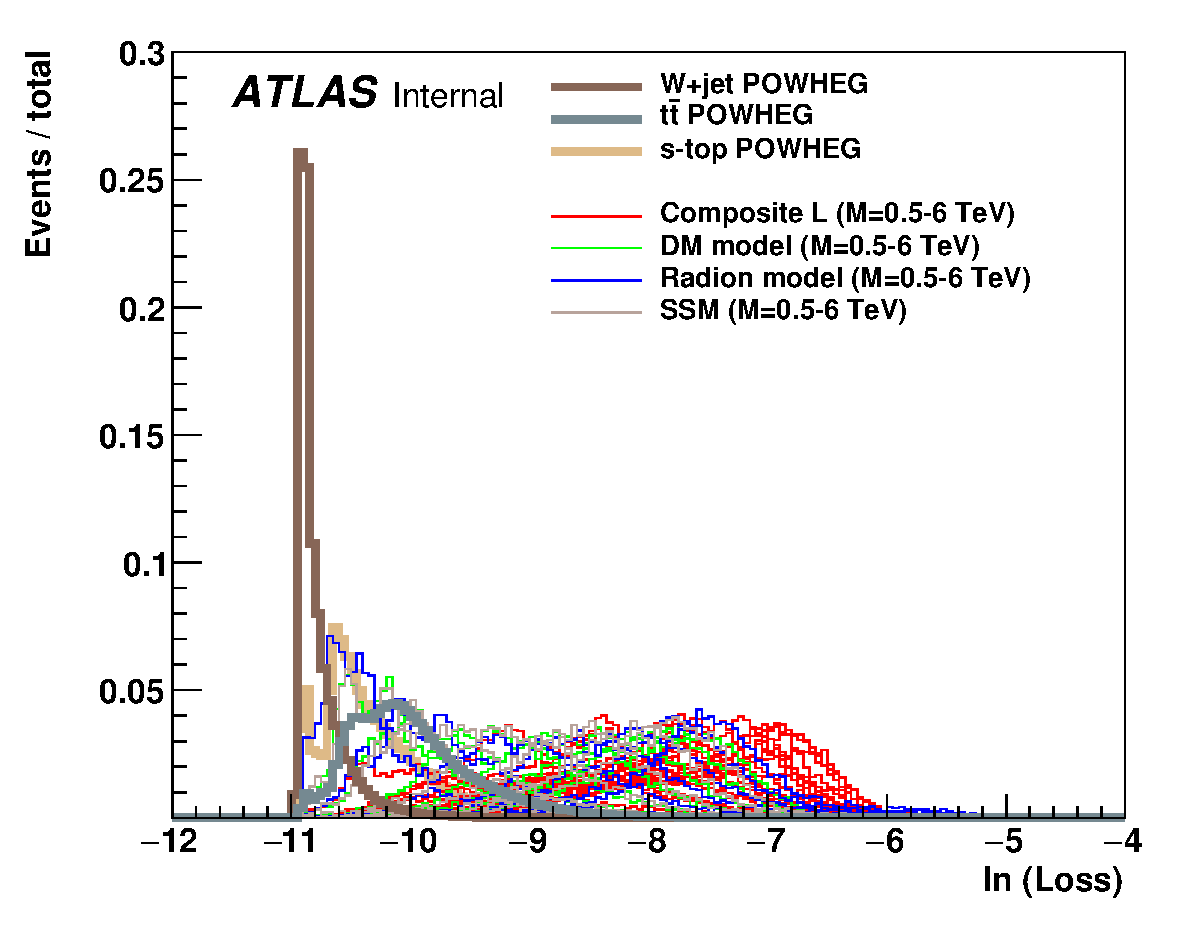
\includegraphics[width=0.45\textwidth]{figs/ch6/ar/plot_loss_mc.pdf}
       }
       \subfloat[Data for autoencoder trained with 1\% of data] {
       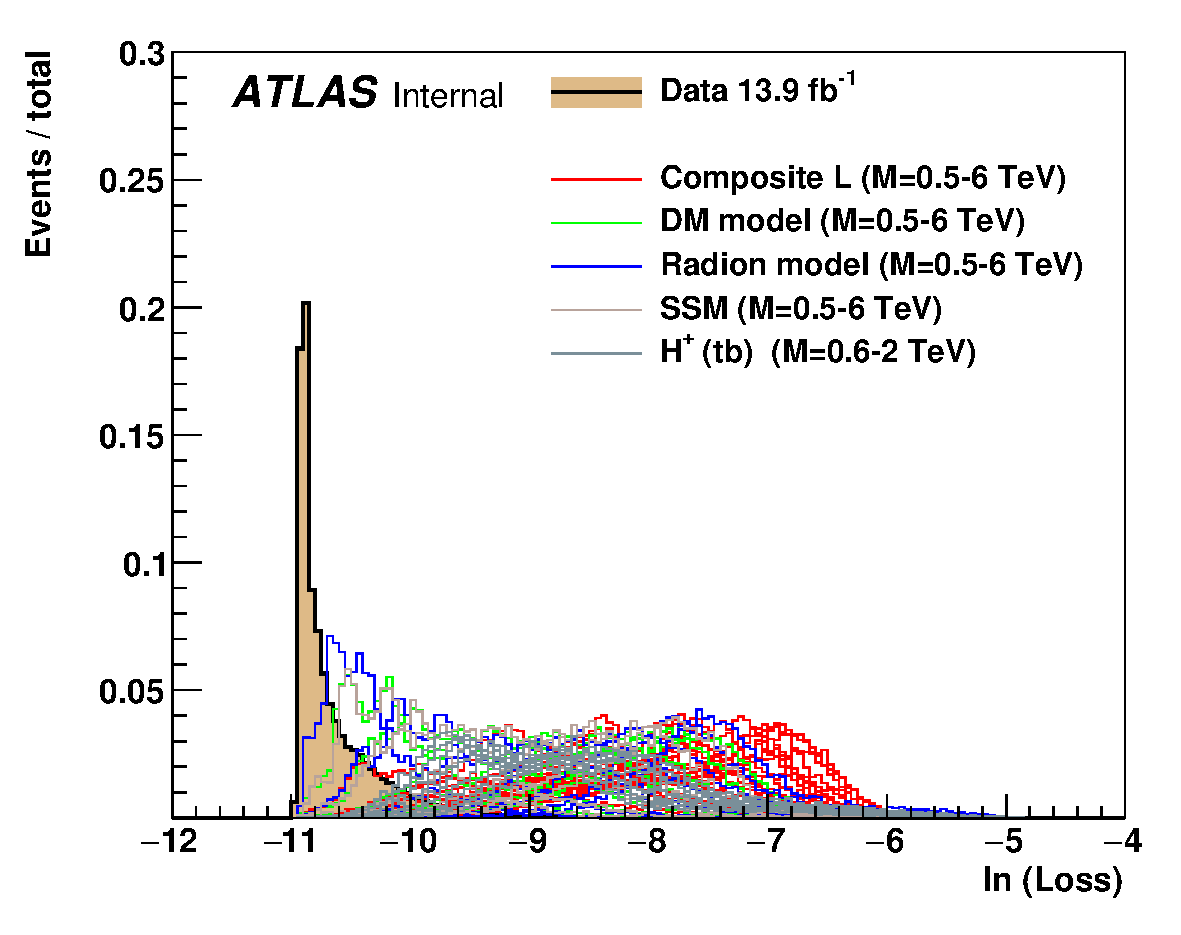
\includegraphics[width=0.45\textwidth]{figs/ch6/ar/plot_loss.pdf}
       }
    \end{center}
    \caption{Distributions of the loss values for the AE trained using 1\% of data.
    (a) The loss distribution for SM and BSM models; (b) The loss distribution for 10\% and BSM models. 
    The BSM models had 20,000 generated events for each mass point in the range 0.5 -- 6 TeV. 
    The larger the mass of the resonance, the further away the line is from the data distribution.
    All the distributions are normalized to the unit area. 
    }
\label{fig:plot_loss_mc}
\end{figure}

\begin{figure}[H]
    \begin{center}
        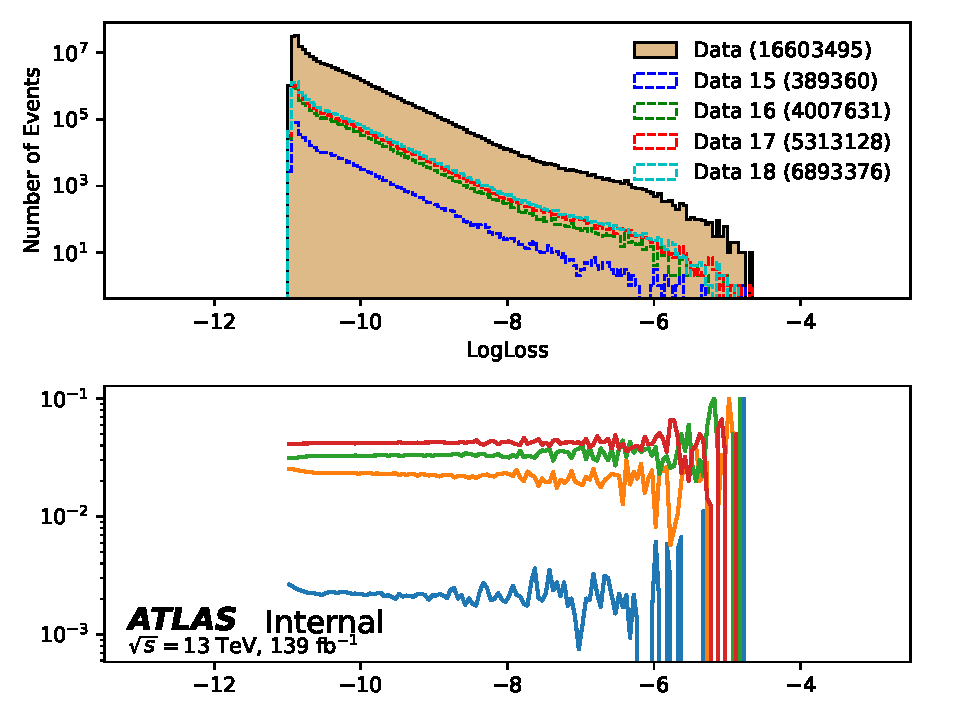
\includegraphics[width=0.8\textwidth]{figs/ch6/logloss_log}
    \end{center}
    \caption{
        Distributions of the loss values for 10\% Run 2 data, scaled by 10 to simulate the actual expected distribution.
        Distributions from each data taking year are shown as well (without multiplying by 10).
        To quantify the difference, the  AE value between individual-year and all-year shapes are computed; they are found to be 'Data 15': 0.485, 'Data 16': 0.491, 'Data 17': 0.505, 'Data 18': 0.502.
        Ratio pad shows the per year shape over full data (note that colors may not be precisely matched).
        They are all close to 0.5, suggesting that different data-taking conditions (e.g.\ pile-up) do not have a large impact on the method.
    }
\label{fig:loss_year}
\end{figure}

\subsection{Determination of Anomaly Region}

The definition of an anomaly region (\gls{ar}) is ambiguous and can be determined depending on the logical needs of the analysis. Within this analysis, the decision was based 
on the example \gls{bsm} models using their theoretical cross-sections times their branching ration (after their acceptances time efficiency corrections). 
The $\sigma \times BR \times Acc  \times  Eff$ were calculated for these models and can be seen in Table~\ref{tab:bsm-cross}. The range 
of these values are within a few hundredths to a few pico-barn. Three \gls{ar}s were defined to ensure sensitivity to a wide range of \gls{bsm} models. These three regions are 
event count bases ranging from 10 pb to 0.1 pb. 

\begin{itemize}
    \item \textbf{10 pb region:} This 10 pb \gls{ar} corresponds to 10 pb $\times \textrm{140} \textrm{fb}^{\textrm{-1}}$=1.4M events. This region has the largest acceptance 
    and is a reasonable choice for many models with leptons in the final state.
    \item \textbf{1 pb region:} This 1 pb \gls{ar} corresponds to 0.14M events of data. This region is less sensitive due to the decrease in statistics but it was expected  
    that the same fit function as the 10 pb \gls{ar} could be used. This assumption is justified since this region has less events and therefore an equation with the same 
    amount or less parameters as the first region should work.
    \item \textbf{0.1 pb region:} This is the third and last \gls{ar} definition and only corresponds to 14K events. This region was included since it corresponds to the upper 
    bound on published experimental limits for dijet mass (including masses with associated lepton or photons). The same fit function will be used for this region as was 
    used in the previous regions.
\end{itemize}    

Since these \gls{ar}s were defined using a count-based assumption, it was possible to define the anomaly score cut numerically. The values were found scanning the 
amount of events bin by bin on the log(\texttt{loss}) anomaly score distribution. The cut values for the 10 pb, 1 pb and the 0.1 pb \gls{ar}s are -9.10, -8.00 and -6.5 respectively and be seen within Table~\ref{tab:test-score-cut}.

\newpage

\begin{table}[H]
    \centering
    \begin{small}
    \begin{tabular}{ |m{2cm} |m{4cm} |m{7cm} |m{2cm} |}
        \hline
        \multicolumn{4}{|c |}{Theoretical Cross Sections times Branching ratios for BSM Models}\\
        \hline
        $\sigma \times \mathrm{BR}$ (pb) & $\sigma \times \mathrm{BR}  \times  Acc  \times  Eff$ (pb) & Model & Reference \\
        \hline\hline
            10       & 2.5                 &  Sequential Standard Model  &  ATLAS  \cite{dijet-res}        \\ 
            1.5      & 0.2                 &  Charged Higgs (hMSSM, $\tan(\beta)=1$)     &   ATLAS  \cite{dijet-res}       \\
            6        & 0.3                  &   Charged Higgs (hMSSM, $\tan(\beta)=0.5$)       &    ATLAS \cite{dijet-res}       \\                     
            0.5      & 0.14                  &   Simplified dark matter model        &    ATLAS  \cite{dijet-res}       \\
            8 (extr) & 1 (extr)           &   Composite lepton model (E=250 GeV) & ATLAS \cite{iso-lep-res}    \\ 
            1.5      & 0.4 (extr)           &   Composite lepton model (E=500 GeV) & ATLAS  \cite{iso-lep-res}    \\
            0.12     & 0.05               &   Technicolor model       &    ATLAS \cite{dijet-res}       \\
            4.5 (extr) & 0.7 (extr)           &   Radion model             &  ATLAS \cite{iso-lep-res}  \\ 
        \hline
    \end{tabular}
    \end{small}
    \caption{Theoretical cross-sections times branching ratios and after $Acc  \times  Eff$ corrections of multiple BSM models near the 400 GeV mass scale that include a single isolated lepton in the final state. The proposed ARs of 10 pb, 1 pb and 0.1 pb covers the cross-sections of most of these models.} 
\label{tab:bsm-cross}
\end{table}

\begin{table}[h!]
    \begin{small}
    %\vspace{5pt}
    \begin{center}	
\begin{tabular}{ |l|l| }
\hline
Cut values & Number of events   \\
\hline	
$-9.00$ & 1146820.0     \\ \hline
$-9.04$ & 1286950.0 \\ \hline
\textbf{$-9.10$} & \textbf{1382880.0}    \\ \hline
$-9.12$ & 1626590.0 \\ \hline
$-9.15$ & 1828930.0  \\ \hline
$-9.20$ & 1828930.0  \\ \hline
\end{tabular}
\begin{tabular}{ |l|l| }
\hline
Cut values & Number of events   \\
\hline
$-7.95$ & 132090.0  \\ \hline
\textbf{$-8.0$} & \textbf{143730.0}     \\ \hline
$-8.02$ & 157050.0     \\ \hline
$-8.10$ & 171040.0     \\ \hline
\end{tabular}
\begin{tabular}{ |l|l| }
\hline
Cut values & Number of events   \\
\hline
$-6.40$ & 11260.0    \\ \hline
$-6.45$ & 12450.0 \\ \hline
\textbf{$-6.50$}  & \textbf{13520.0}  \\ \hline
$-6.55$ & 14770.0   \\ \hline
$-6.60$ & 16020.0   \\ \hline
$-6.65$ & 17600.0   \\ \hline
\end{tabular}
\end{center}
\end{small}
\caption{Number of events after the anomaly score cut for each AR. The 10 pb BSM region is defined by the logarithm of the loss function > -9.10, the 1 pb is defined by the logarithm loss > -8.00, and likewise for the 0.1 pb logarithm loss > -6.50 }
\label{tab:test-score-cut}
\end{table}
\newpage

Multiple mass hypotheses of each example \gls{bsm} model was observed using these defined \gls{ar} regions in order to test the $\textrm{S}/\sqrt{\textrm{B}}$ after the anomaly score cut. Figure~\ref{fig:bsm-loss} shows comparisons for each five 
\gls{bsm} model previously described. These mass hypotheses of $\textrm{Z}' / \textrm{W}' / \textrm{H}^{+}$ range from 0.5 $-$ 6 TeV. The larger the mass resonance (closer to 6 TeV), the larger the loss from the 
\gls{ae} is expected. The number of events for each model were estimated using their cross-sections and the luminosity. Figure~\ref{fig:sb-comp} shows the integrated $\textrm{S}/\textrm{B}$ and $\textrm{S}/\sqrt{\textrm{B}}$ for all the \gls{bsm} signals stacked. 
The 10 pb cut happens to be near the most optimal $\textrm{S}/\sqrt{\textrm{B}}$ meaning the signal in the calculation is dominated by lower mass resonances. It is worthy to note that this optimal cut would adjust towards the right
from its current position if this calculation only includes higher mass resonances. The fact that the optimal cut is found to be at 10 pb for an inclusive mass resonance range indicates this method with the 
addition of the other two defined \gls{ar}s is a robust strategy.
\newpage

\begin{figure}[H]
    \centering
    \begin{subfigure}[h]{0.45\linewidth}
    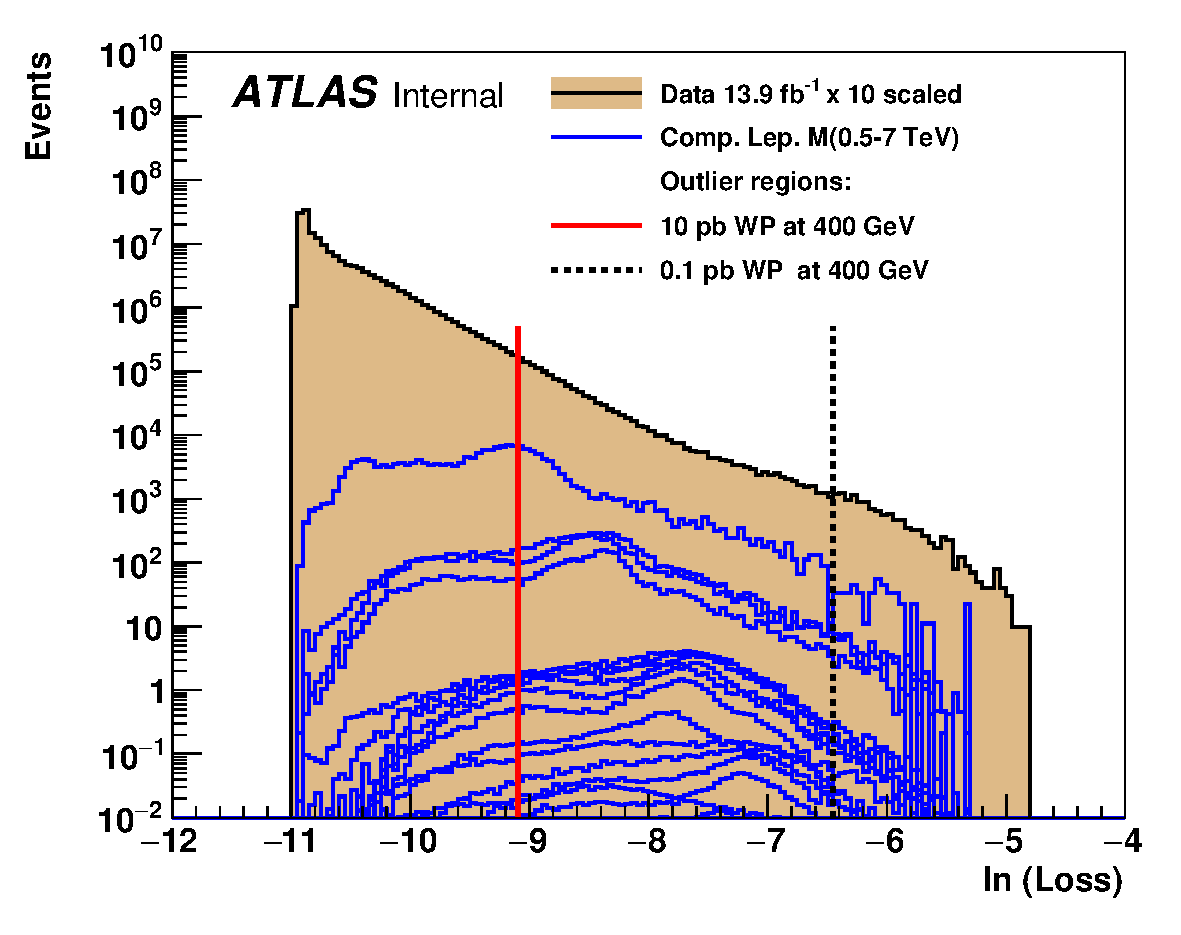
\includegraphics[scale=0.35]{figs/ch6/ar/plot_loss_cut_complep.pdf}%
    \caption{Composite Leptons}
    \end{subfigure}
    \hfill
    \begin{subfigure}[h]{0.45\linewidth}
    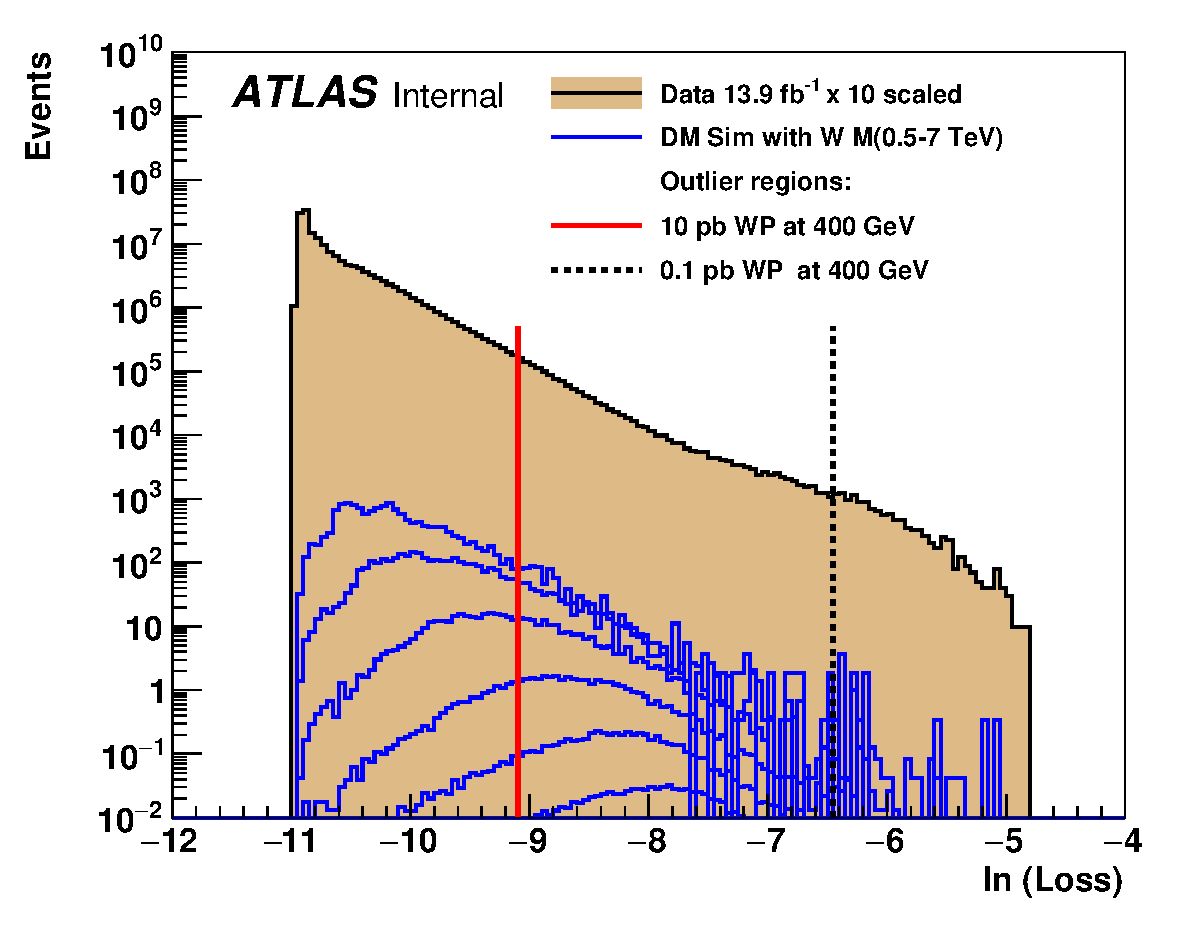
\includegraphics[scale=0.35]{figs/ch6/ar/plot_loss_cut_dmsim.pdf}%
    \caption{Dark Matter}
    \end{subfigure}
    \hfill
    \begin{subfigure}[h]{0.45\linewidth}
    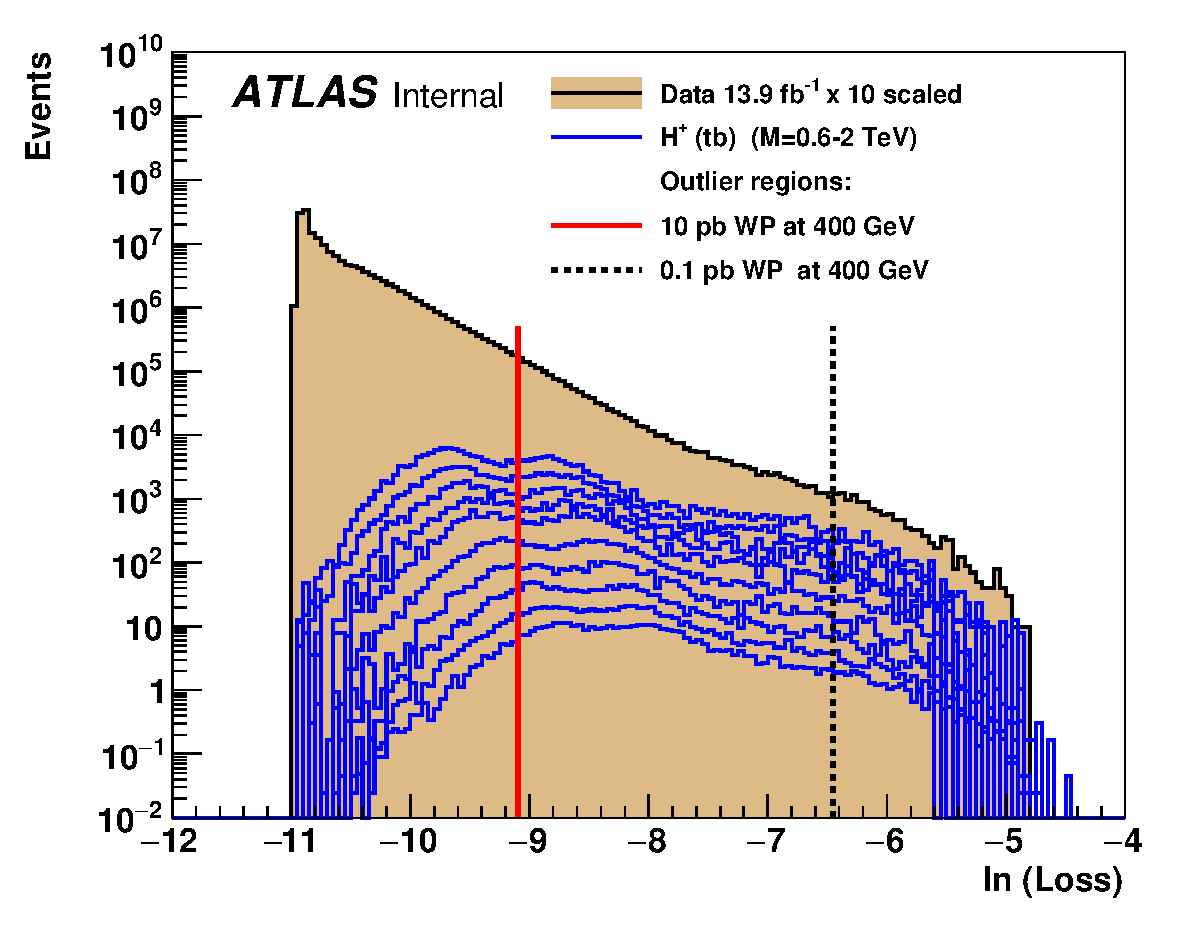
\includegraphics[scale=0.35]{figs/ch6/ar/plot_loss_cut_hsplus.pdf}%
    \caption{Charged Higgs}
    \end{subfigure}
    \hfill
    \begin{subfigure}[h]{0.45\linewidth}
    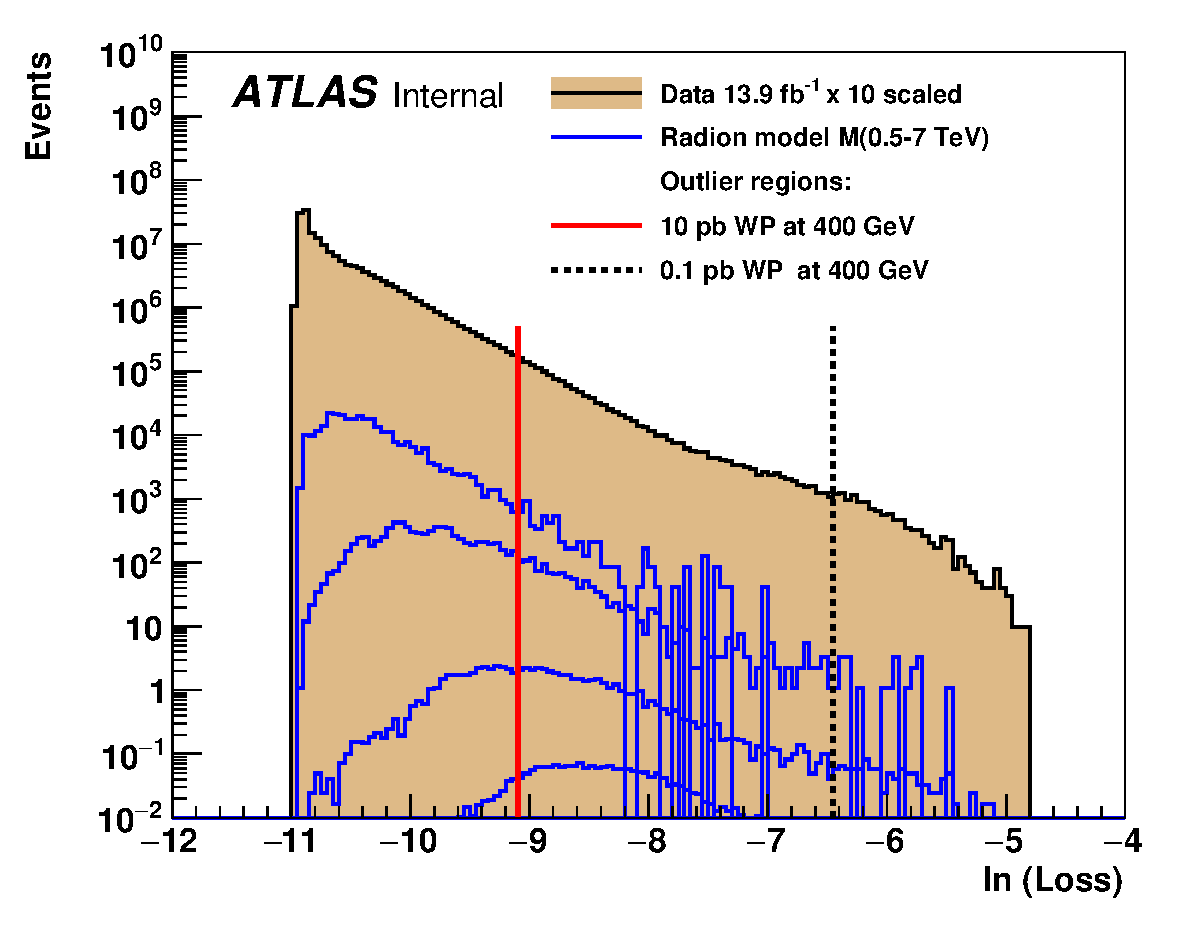
\includegraphics[scale=0.35]{figs/ch6/ar/plot_loss_cut_radion.pdf}%
    \caption{Radion}
    \end{subfigure}
    \hfill
    \begin{subfigure}[h]{0.45\linewidth}
    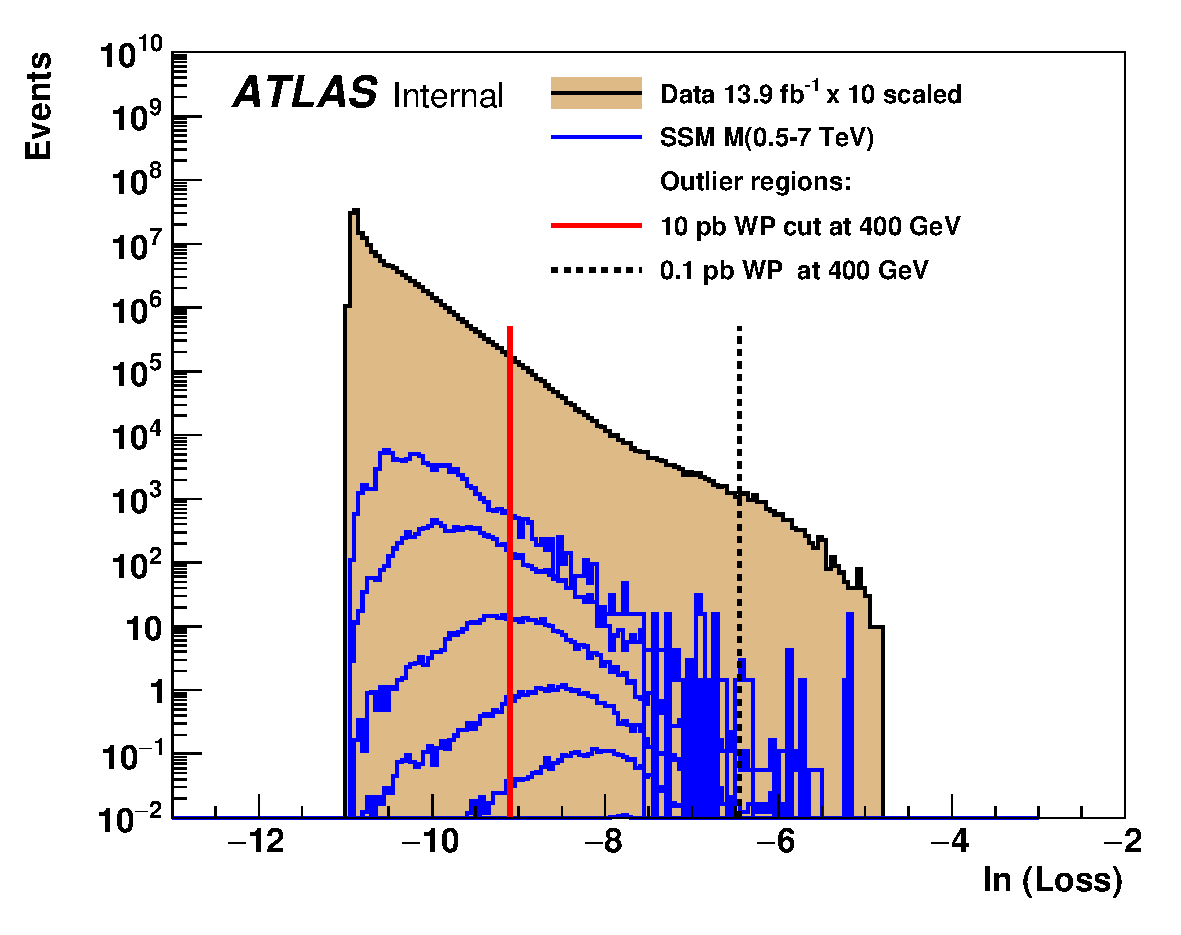
\includegraphics[scale=0.35]{figs/ch6/ar/plot_loss_cut_ssm.pdf}%
    \caption{Sequential SM}
    \end{subfigure}
    \hfill
    \caption{Distributions of the loss values using the trained nominal AE with different BSM models. The mass resonance range between 0.5 - 6 TeV with higher loss values for larger mass resonances. The data distribution uses 10\% of Run 2 data that is scaled by 10 to show the expected shape of the full Run 2 dataset. Two vertical lines shows the max and min AR regions (10 pb and 0.1 pb)}
\label{fig:bsm-loss}
\end{figure}


\begin{figure}[ht]
    \centering
    \begin{subfigure}[h]{0.45\linewidth}
    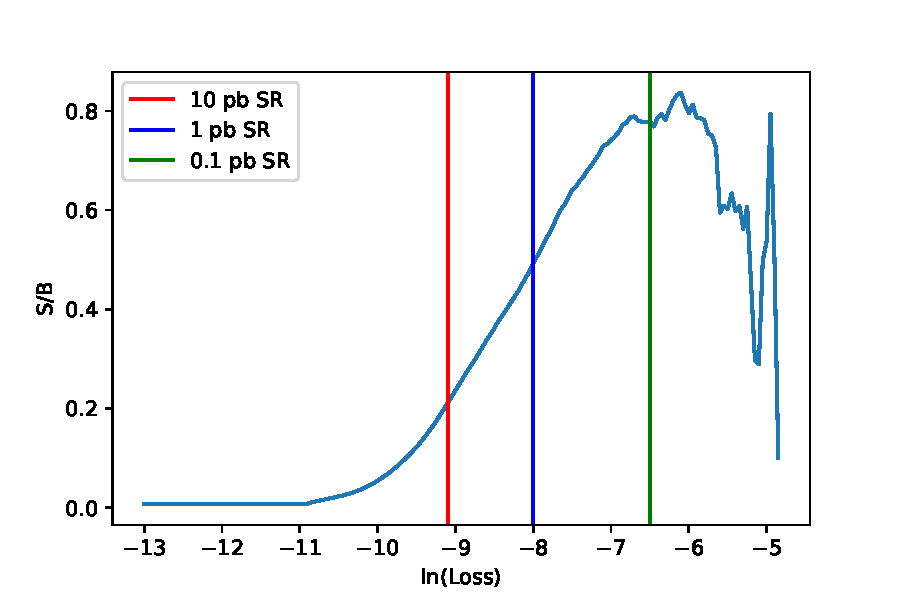
\includegraphics[scale=0.45]{figs/ch6/ar/BSMall_SoverB_vs_loss.pdf}%
    \caption{$\textrm{S}/\textrm{B}$ for stacked BSM models}
    \end{subfigure}
    \hfill
    \begin{subfigure}[h]{0.45\linewidth}
    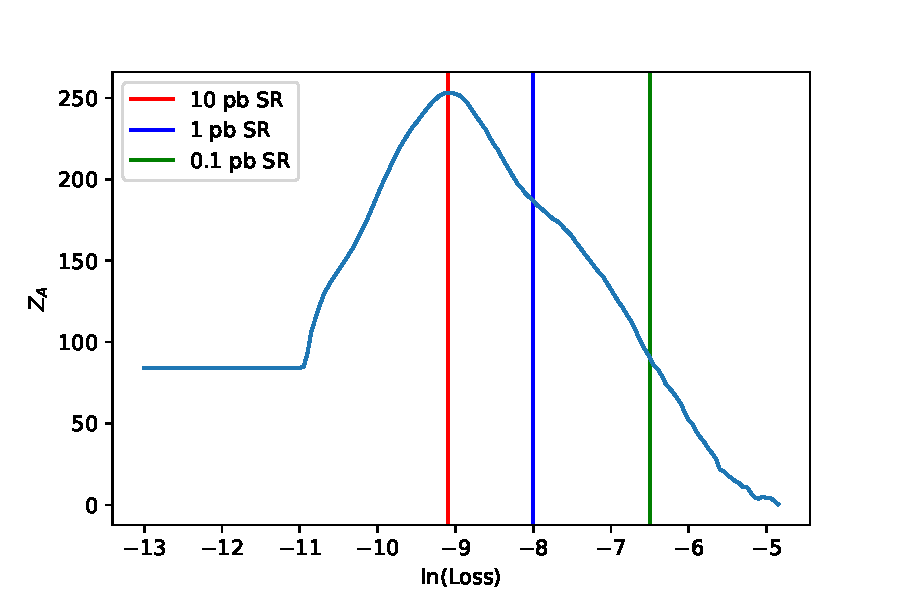
\includegraphics[scale=0.45]{figs/ch6/ar/BSMall_ZA_vs_loss.pdf}%
    \caption{$\textrm{S}/\sqrt{\textrm{B}}$ for stacked BSM models}
    \end{subfigure}
    \hfill
    \caption{Integrated $\textrm{S}/\textrm{B}$ and $\textrm{S}/\sqrt{\textrm{B}}$ scans for the stack BSM models show in Figure~\ref{fig:bsm-loss}. S is calculated as the integral of the BSM signal from a given x value to $+$infinity; B is calculated as the integral of the data at a give value x to $+$infinity. The colored vertical lines show the positions of the AR cuts. }
\label{fig:sb-comp}
\end{figure}

\section{Analysis of Anomaly Regions}

The objects of interest are nine di-object invariant masses. These masses are:

\begin{enumerate}
    \item Invariant mass of 2-jets ($\textrm{m}_{\textrm{jj}}$)
    \item Invariant mass of a jet and a b-jet ($\textrm{m}_{\textrm{jb}}$)
    \item Invariant mass of two b-jets ($\textrm{m}_{\textrm{bb}}$)
    \item Invariant mass of a jet and an electron ($\textrm{m}_{\textrm{je}}$)
    \item Invariant mass of a jet and muon ($\textrm{m}_{\textrm{jμ}}$)
    \item Invariant mass of a jet and photon ($\textrm{m}_{\textrm{j}\gamma}$)
    \item Invariant mass of a b-jet and an electron ($\textrm{m}_{\textrm{be}}$)
    \item Invariant mass of a b-jet and a muon ($\textrm{m}_{\textrm{jμ}}$)
    \item Invariant mass of a b-jet and a photon ($\textrm{m}_{\textrm{j}\gamma}$)
\end{enumerate}

The approach here is to use \gls{mc} simulations of $t\bar{t}$ and W+jets (samples listed in Appendix~\ref{appendix:mc-ad}) combined with a data-driven multi-jet for \gls{sm} background estimations. With this background a fit function is applied to establish the 
estimated shape of this background. The function is then tested further using a variety of statistical tests and then finally cross-checked with a 10\% data sample (separate events from training) in a step 
called a stage-1 unblinding before being fully unblinded. 

\subsection{Background Modeling}

The bin widths of the invariant masses are chosen to match the \gls{jes} of the \gls{atlas} detector. The bin widths are approximately equal to the theorized model width at a given mass with increasing bin size 
that widen with increasing invariant mass from 13 GeV to 120 GeV. The fit procedure and function in this analysis follows the procedure outlined in \cite{fit-hypo}. This fit hypothesis (Eq.~\ref{eq:fit-function}) is used to establish the 
background shape.

\begin{equation}
    f(x) = p_1 (1 - x)^{p_2} x^{p_3 + p_4\ln x + p_5 \ln^2 x},
\label{eq:fit-function}
\tag{6.6}
\end{equation}

where $x \equiv $ \mjj$ /\sqrt{s}$ and the $p_i$\ are five free parameters to be estimated. Having fit function with up to five parameters allows for more flexibility at low \mjj. This fit function from herein 
is referred to as ``p5''. In addition, in addition ``p4'' ($p_5=0$) and ``p6'' functions (after multiplying the function by $x^{p_6 \ln^3 x}$) are studied. Using a function with more parameters, such
as the p6 can be dangerous as high parameter functions are more likely to absorb possible signal. Therefore, statistical tests are utilized to ensure the optimized amount of parameters are found while also 
testing the function on each invariant mass distribution since it's possible the fit could fail on a distribution with low statistics. 
\par
An alternative fit function is proposed to evaluate the systematic uncertainties related to the function to fit the background. The chosen alternative function can be seen in Eq.~\ref{eq:function_alt} as it resembles the used p5 fit 
function that is later used to estimate the background. This function has shown to give an alternative description of the tail in the \mjj distribution, compared to the p5 function \cite{alt-fit-hypo}. 

\begin{equation}
    f(x)^{alt} = p_1 (1 - x)^{p_2} x^{p_3 + p_4\ln x + p_5 /\sqrt{x}},
\label{eq:function_alt}
\tag{6.7}
\end{equation}

To fit the binned histograms, the Minuit/ROOT program was used. histograms with event yields were divided by the bin width, this was fed as inputs into the Minuit/ROOT program to obtain fit parameters. 
To ensure the most optimal minimization of the fit function, the following procedure was used. First, the fit parameters are initialized randomly and the fit is performed. The fit criteria requires a $\chi^{\textrm{2}}/\textrm{ndf}<$1.4
to be considered as the correct parameter space. If the fit doesn't converge to this criteria, a new fit trial begins starting from the parameters as the previous fit. 100 of these trials are then performed, if a 
fit cannot be found with a $\chi^{\textrm{2}}/\textrm{ndf}<$1.4, the parameters are then randomly initialized and the procedure starts over. This iterative fitting procedure is then repeated a maximum of 100 times
to obtain correct parameter space. If the criteria of $\chi^{\textrm{2}}/\textrm{ndf}<$1.4 is never obtained, then the claim is that this fit function is unable to describe the background shape.
/par
Additional tests are performed once reasonable fitting parameters are found via this method. To ensure the function isn't ``too flexible'', one of these tests are spurious signal tests which are 
conducted to help verify the chosen form of the function. This procedure is non-trivial due to the fact that the chosen number of parameters must work for all nine invariant mass background shapes. If there 
are not enough parameters, the shapes won't converge into a viable fit, whereas if there are too many variables, it's possible that an hints of resonances may be hidden within the fit. 

\subsection{Statistical Tests}

Several statistical tests are ran to ensure the quality of fit. These tests are ran on the normality of distributions of scaled residuals, $S_i = \frac{\text{yields} - \text{pred}}{\Delta \text{yields}}$, or commonly 
referred as ``pulls''. These pull values are then tested to verify that they follow a normal distribution with $\sigma$=1 and mean of 0. Seven tests are ran in all. These tests and their criteria are:

\begin{enumerate}
    \item $\chi^{\textrm{2}}/\textrm{ndf}<$1.4
    \item Kolmogorov-Smirnov (KS) test has a probability $>$ 0.3
    \item Gaussian fit of the pulls has a mean of 0 within the  1$\sigma$ statistical uncertainty
    \item Gaussian fit of the pulls has a standard deviation with the value of 1 (within the 1$\sigma$ uncertainty)
    \item Skewness value is 0 within the 1$\sigma$ uncertainty
    \item Kurtosis value is 0 within the 1$\sigma$ uncertainty
    \item Shapiro-Wilk's test shows the probability above 0.7
\end{enumerate}

First, as Gaussian fit to the pulls $S_i$ is performed to make sure that the peak and the width of the fitted Gaussian has a mean of 0 with a width of 1. A $\chi^{\textrm{2}}$ test is ran to verify that the Gaussian
fit of the $S_i$ is acceptable. The Shapiro-Wilk's test is used to detect all departures from normality without using the Gaussian fit. The Kolmogorov-Smirnov test is used to determine if the pull data is 
normally distributed. In addition, \textit{skewness} is checked that measures the relative size of both tails along with the \textit{kurtosis} test that measures whether if the distribution is heavy-tailed 
relative to the normal distribution. The skewness and Kurtosis tests are equal to zero for an normal distribution, so if the pull's tests are not close to zero then the test is considered failed. 
\par
To determine whether the number of chosen parameters for the function is optimized, the F-test is utilized. This test verifies if the default function against alternative, more complex options \cite{f-test}. If no significant 
improvements are seen for the \gls{mc} control regions, the function with lower complexity is prioritized since lower parameter functions lead to more stable fits and less likely to lead to spurious signals. 
All tests described here are performed on the \gls{sm} \gls{mc} plus the data-driven multi-jet background. In addition, the F-test is performed on real data in the 1 pb and the 0.1 pb to reduce parameters. 
\par
Once a fit function is tested and has proved to be viable for background estimation, a BumpHunter (\gls{bh}) statistical test is performed to check if there are any significant deviations from the background, 
i.e. possible \gls{bsm} resonances. This test is calculated by looking at the discrepancy in windows of varying width for all data bins and is sensitive to whether discrepancies in neighboring bins have sign outcome.
This test also reports a final \textit{p}-value as all possible locations for an excess is considered, choosing the lowest value. The frequentist approach that is used in this analysis involves calculating this \gls{bh} statistic for many 
pseudo-experiments, having the lowest \textit{p}-value outcome originate from different locations. The final \textit{p}-value is formed from the union of the smallest \textit{p}-values calculated from these pseudo-experiments. 
\par
When applying the \gls{bh} test to our \gls{ar}s, the procedure looks for each N possible intervals of \mjj, a local \textit{p}-value is calculated from a unique hypothesis test 
statistic. \gls{bh} then combines each of the N hypotheses for form a new hypothesis test, calculating the minimum \textit{p}-value amongst all the tests. These are then 
combined into a global \textit{p}-value and transformed into a significance assuming that the bin-by-bin distribution follows a Poisson distribution. Pseudo-experiments as 
described above are then used to determine the most significant local excess and a global significance. This test is used after a reasonable fit function is found to describe 
the background estimation in order to find any deviances after unblinding. 

\subsection{Background Fit Studies}\label{sec:bkg-fit-studies}

The background estimation in these studies are a combination of $t\bar{t}$, W+jets and the \gls{le-cr}. These 
figures show all nine invariant mass distributions in the 10 pb \gls{ar} (fit studies looking at the other \gls{ar}s, 1 pb and 0.1 pb, can be found in Appendices \ref{appendix:1pb-fit-studies} and \ref{appendix:01pb-fit-studies}).
Three fit functions were tested, a p4, p5 and a p6. The statistical tests and discussed in the previous section for the pull values are shown in Table~\ref{tab:stat-quantities-10PB-SMMCplusCR} for the 10 pb \gls{ar}
(Table~\ref{tab:stat-quantities-1PB-SMMCplusCR} and Table~\ref{tab:stat-quantities-01PB-SMMCplusCR} in Appendix for the other two \gls{ar}s). These studies show that the p5 performs the best. The three fit functions tested are:

\begin{itemize}
    \item $p4$: $f(x) = p_1 (1 - x)^{p_2} x^{p_3 + p_4\ln x}$;
    \item $p5$: $f(x) = p_1 (1 - x)^{p_2} x^{p_3 + p_4\ln x + p_5 \ln^2 x}$;
    \item $p6$: $f(x) = p_1 (1 - x)^{p_2} x^{p_3 + p_4\ln x + p_5 \ln^2 x + p_6 \ln^3 x}$.
\end{itemize}

To construct the \gls{mc}+\gls{le-cr}, the distribution of the \gls{le-cr} was scaled such that it fills the gap between data (before \gls{ar} cut) and the \gls{mc} 
predictions for $t\bar{t}$ and W+jets. The data used was 10\% of Run 2 and then scaled by 10 to show the full dataset shape as seen in Figure~\ref{fig:mjj-fit-data}. The scaling factor applied to the 
\gls{le-cr} is (\textit{data}-\textit{MC})/\textit{a}, where \textit{a} is the value of the integral of the \gls{le-cr}. After applying the 10 pb \gls{ar} cut to 
the combination of the \gls{mc}+\gls{le-cr}, the fitting procedure for all the tested functions was performed on each invariant mass. The results of the 
statistical tests for these three functions on the 10 pb \gls{ar} can be seen in Table~\ref{tab:stat-quantities-10PB-SMMCplusCR}. The studies on the 1 pb and 0.1 pb can be found in Appendix\ref{appendix:1pb-fit-studies}-\ref{appendix:01pb-fit-studies}. 

\begin{figure}[ht]
    \centering
    \begin{subfigure}[h]{0.4\linewidth}
    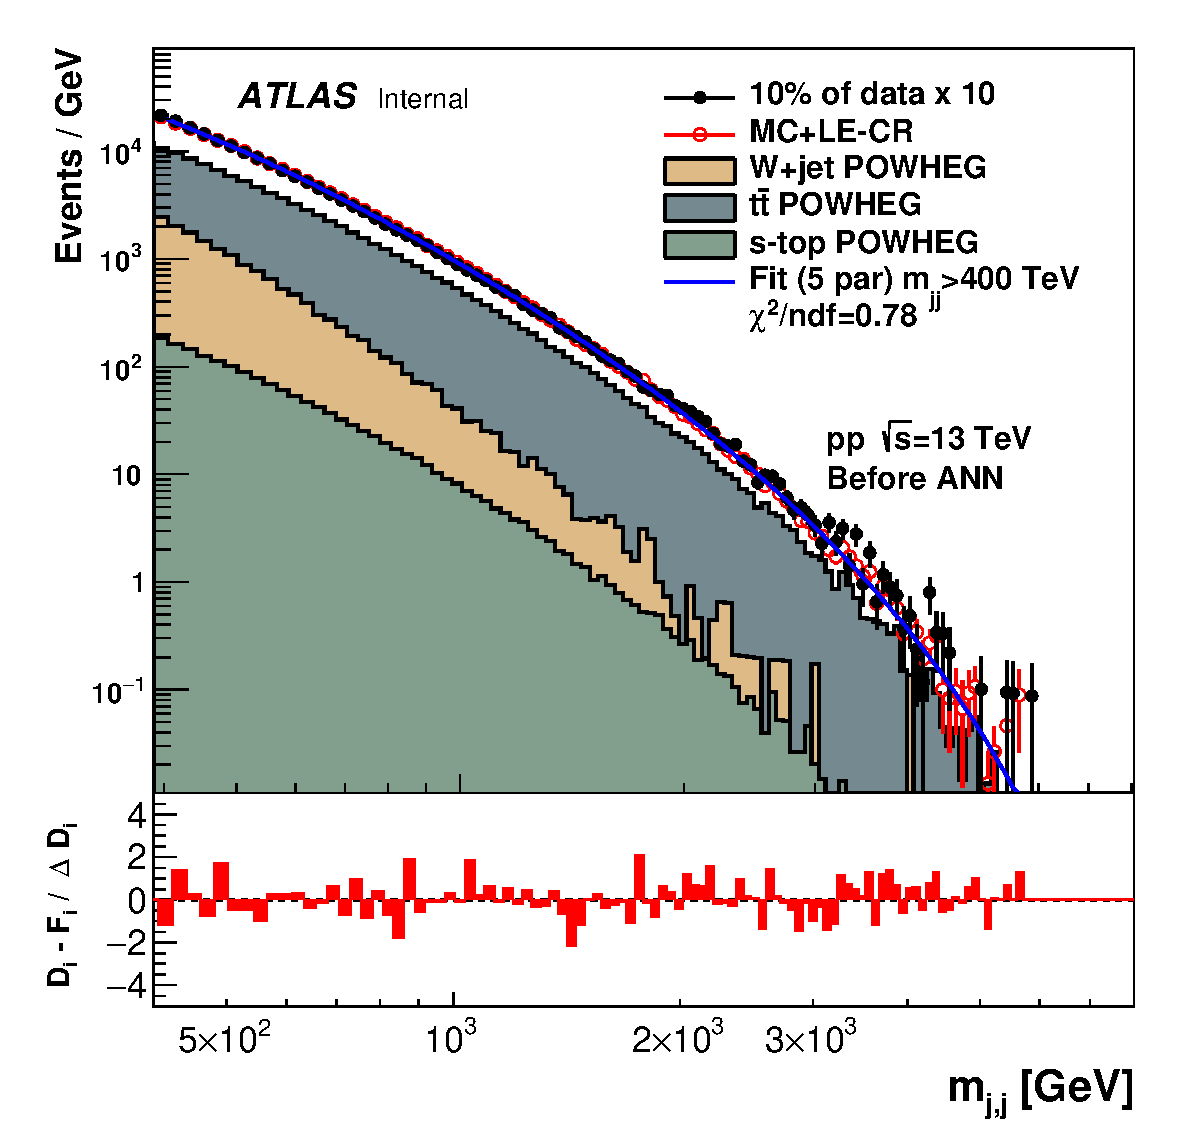
\includegraphics[scale=0.32]{figs/ch6/fit/mass_jj_mcCR_before_scale.pdf}%
    \caption{Before 10 pb AR cut}
    \end{subfigure}
    \hfill
    \begin{subfigure}[h]{0.45\linewidth}
    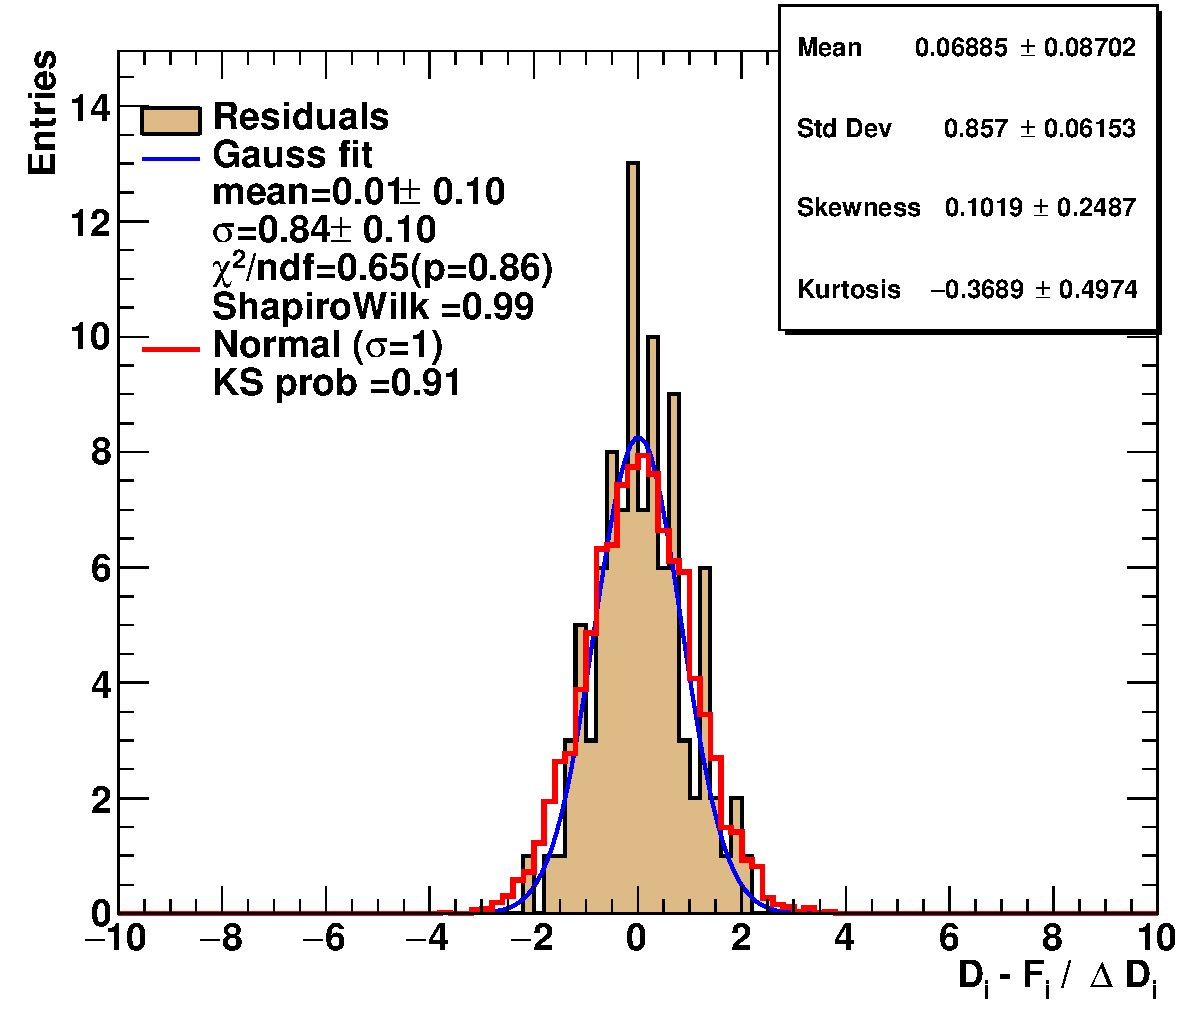
\includegraphics[scale=0.35]{figs/ch6/fit/mass_jj_mcCR_before_scale_residuals.pdf}%
    \caption{Pulls before 10 pb AR cut}
    \end{subfigure}
    \hfill
    \caption{The distribution of $\textrm{m}_{\textrm{jj}}$ before the 10 pb AR cut. The red dots show the MC+LE-CR data together with the p5 fit. }
\label{fig:mjj-fit-data}
\end{figure}

\begin{multicols}{3}
    \begin{itemize}
    \item Figure~\ref{fig:mjj-fit-pulls} 10pb \mjj
    \item Figure~\ref{fig:mjb-fit-pulls} 10pb \mjb
    \item Figure~\ref{fig:mbb-fit-pulls} 10pb \mbb
    \item Figure~\ref{fig:mje-fit-pulls} 10pb \mje
    \item Figure~\ref{fig:mjm-fit-pulls} 10pb \mjmu
    \item Figure~\ref{fig:mjg-fit-pulls} 10pb \mjph
    \item Figure~\ref{fig:mbe-fit-pulls} 10pb \mbe
    \item Figure~\ref{fig:mjm-fit-pulls} 10pb \mbmu
    \item Figure~\ref{fig:mbg-fit-pulls} 10pb \mbph
    \end{itemize}
 \end{multicols}

\newpage

\def\tableCaption{Statistical quantities for SM MC + CR fit}

\begin{table}[!htbp]
   \begin{center}
      \begin{scriptsize}
      \begin{tabular}{|c|c|c|c|c|c|c|c|c|c|c|c|}
         \hline
         {Mass} & {region} & {p} & {Fit $\chi^2$} & {Pull $\mu$} & {$\Delta\mu$} & {$\sigma$} & {$\Delta\sigma$} & {Gaus $\chi^2$} & {KS} & {Shapiro}  \\
         % \midrule
         % $\Mjj$ & 20 pb & 4 & 1.241783 & 0.372261 & 0.158871 & 1.061787 & 0.156896 & 0.814828 & 0.962140 & 0.958880 \\
         % $\Mjb$ & 20 pb & 4 & 1.348155 & 0.228527 & 0.130358 & 1.048940 & 0.133652 & 0.859302 & 0.614734 & 0.955352 \\
         % $\Mbb$ & 20 pb & 4 & 1.299993 & 0.494530 & 0.145545 & 0.869209 & 0.337489 & 1.286050 & 0.006117 & 0.935971 \\
         % $\Mje$ & 20 pb & 4 & 2.641893 & 0.195809 & 0.230595 & 1.684589 & 0.312043 & 0.920687 & 0.080787 & 0.991116 \\
         % $\Mjm$ & 20 pb & 4 & 0.935827 & 0.132905 & 0.087658 & 0.602263 & 0.095498 & 1.672907 & 0.811660 & 0.979955 \\
         % $\Mjg$ & 20 pb & 4 & 1.224005 & -0.151274 & 0.134722 & 1.097871 & 0.139473 & 0.637132 & 0.968877 & 0.993533 \\
         % $\Mbe$ & 20 pb & 4 & 0.937459 & 0.112502 & 0.151966 & 1.023924 & 0.167777 & 1.163444 & 0.893562 & 0.956552 \\
         % $\Mbm$ & 20 pb & 4 & 1.148871 & 0.363368 & 0.225413 & 1.220507 & 0.422497 & 1.190430 & 0.179341 & 0.981366 \\
         % $\Mbg$ & 20 pb & 4 & 0.860249 & 0.340316 & 0.106324 & 0.706506 & 0.108286 & 0.796108 & 0.323092 & 0.948463 \\
         % \midrule
         % $\Mjj$ & 20 pb & 5 & 0.939936 & 0.202880 & 0.167960 & 1.070181 & 0.183370 & 1.025595 & 0.991272 & 0.982271 \\
         % $\Mjb$ & 20 pb & 5 & 1.286332 & 0.177649 & 0.124803 & 1.012652 & 0.130596 & 0.898115 & 0.614734 & 0.983926 \\
         % $\Mbb$ & 20 pb & 5 & 1.093123 & 0.358919 & 0.158919 & 1.014795 & 0.165521 & 1.219283 & 0.057420 & 0.951658 \\
         % $\Mje$ & 20 pb & 5 & 1.257110 & 0.099816 & 0.177017 & 1.304808 & 0.189597 & 1.101121 & 0.308834 & 0.986169 \\
         % $\Mjm$ & 20 pb & 5 & 0.966783 & -0.034972 & 0.136980 & 0.981749 & 0.149815 & 0.679193 & 0.807649 & 0.982734 \\
         % $\Mjg$ & 20 pb & 5 & 0.950975 & 0.437368 & 0.129980 & 0.951766 & 0.134269 & 1.465126 & 0.078553 & 0.959805 \\
         % $\Mbe$ & 20 pb & 5 & 0.852128 & 0.381678 & 0.350013 & 1.311341 & 0.327514 & 1.426666 & 0.796893 & 0.967672 \\
         % $\Mbm$ & 20 pb & 5 & 1.103166 & 0.111524 & 0.231942 & 1.336972 & 0.227344 & 0.919342 & 0.137127 & 0.976889 \\
         % $\Mbg$ & 20 pb & 5 & 0.703805 & 0.070777 & 0.113688 & 0.797121 & 0.111281 & 0.854572 & 0.449807 & 0.980126 \\
         % \midrule
         % $\Mjj$ & 20 pb & 6 & 0.958736 & 0.248024 & 0.153579 & 1.036828 & 0.168795 & 1.024001 & 0.991272 & 0.977715 \\
         % $\Mjb$ & 20 pb & 6 & 1.281121 & 0.135524 & 0.126004 & 1.018146 & 0.140622 & 0.738419 & 0.785662 & 0.981597 \\
         % $\Mbb$ & 20 pb & 6 & 1.246056 & 0.126215 & 0.317241 & 1.564866 & 0.376284 & 1.878865 & 0.030365 & 0.958929 \\
         % $\Mje$ & 20 pb & 6 & 1.052496 & 0.000097 & 0.167781 & 1.193179 & 0.166497 & 0.745597 & 0.792332 & 0.990251 \\
         % $\Mjm$ & 20 pb & 6 & 0.967763 & 0.115453 & 0.177765 & 1.147995 & 0.185684 & 1.443809 & 0.864477 & 0.977291 \\
         % $\Mjg$ & 20 pb & 6 & 0.950110 & 0.218055 & 0.108876 & 0.846002 & 0.106625 & 1.128963 & 0.379200 & 0.966174 \\
         % $\Mbe$ & 20 pb & 6 & 0.882272 & 0.537800 & 0.354982 & 1.357165 & 0.294808 & 0.606337 & 0.610562 & 0.968305 \\
         % $\Mbm$ & 20 pb & 6 & 1.111754 & 0.252187 & 0.203130 & 1.177482 & 0.225574 & 1.173883 & 0.230690 & 0.985383 \\
         % $\Mbg$ & 20 pb & 6 & 0.712115 & 0.352343 & 0.198622 & 1.124331 & 0.230377 & 0.676621 & 0.509423 & 0.964623 \\
         \hline
         \mjj & 10 pb & 4 & 1.350225 & 0.188249 & 0.118766 & 1.000243 & 0.118738 & 0.668667 & 0.838354 & 0.967003 \\
         \mjb & 10 pb & 4 & 1.654758 & 0.288073 & 0.174609 & 1.184496 & 0.190722 & 1.266895 & 0.204681 & 0.947339 \\
         \mbb & 10 pb & 4 & 1.339481 & 0.259308 & 0.184551 & 1.060607 & 0.198495 & 1.115230 & 0.030365 & 0.931438 \\
         \mje & 10 pb & 4 & 1.882063 & 0.181406 & 0.190882 & 1.402343 & 0.218868 & 0.983200 & 0.122363 & 0.938806 \\
         \mjmu & 10 pb & 4 & 0.954052 & 0.267345 & 0.109163 & 0.742488 & 0.134621 & 0.777527 & 0.349305 & 0.945133 \\
         \mjph & 10 pb & 4 & 0.773106 & 0.002398 & 0.130570 & 1.014041 & 0.135647 & 0.469318 & 0.798588 & 0.983349 \\
         \mbe & 10 pb & 4 & 0.972373 & 0.545587 & 0.291598 & 1.414412 & 0.274838 & 0.768124 & 0.610562 & 0.970631 \\
         \mbmu & 10 pb & 4 & 1.494746 & 0.706422 & 0.423572 & 1.646267 & 0.487647 & 0.663357 & 0.103588 & 0.967773 \\
         \mbph & 10 pb & 4 & 0.824516 & 0.218063 & 0.156917 & 0.965077 & 0.163884 & 0.914854 & 0.200394 & 0.962123 \\
         \hline
         \mjj & 10 pb & 5 & 1.009592 & 0.145683 & 0.122463 & 0.986835 & 0.109409 & 0.841748 & 0.915870 & 0.978346 \\
         \mjb & 10 pb & 5 & 1.195392 & 0.167570 & 0.169755 & 1.194622 & 0.210126 & 1.141865 & 0.449203 & 0.991612 \\
         \mbb & 10 pb & 5 & 0.903178 & 0.314245 & 0.105781 & 0.800464 & 0.094230 & 0.515502 & 0.302650 & 0.954691 \\
         \mje & 10 pb & 5 & 1.226098 & 0.185050 & 0.126940 & 0.989509 & 0.112932 & 1.166452 & 0.455442 & 0.975749 \\
         \mjmu & 10 pb & 5 & 0.969384 & 0.402821 & 0.135216 & 0.923938 & 0.133419 & 0.808335 & 0.061480 & 0.936338 \\
         \mjph & 10 pb & 5 & 0.781334 & 0.028170 & 0.130375 & 1.004669 & 0.138376 & 0.590685 & 0.630669 & 0.983825 \\
         \mbe & 10 pb & 5 & 0.795931 & 0.331966 & 0.188702 & 1.092156 & 0.177057 & 0.671857 & 0.931749 & 0.973960 \\
         \mbmu & 10 pb & 5 & 1.115614 & 0.594871 & 0.411939 & 1.518365 & 0.440538 & 0.744476 & 0.365553 & 0.976348 \\
         \mbph & 10 pb & 5 & 0.696946 & 0.063387 & 0.120639 & 0.860113 & 0.104889 & 0.402123 & 0.926549 & 0.987653 \\
         \hline
         \mjj & 10 pb & 6 & 0.954477 & 0.166474 & 0.114638 & 0.936988 & 0.106383 & 0.956339 & 0.974623 & 0.985057 \\
         \mjb & 10 pb & 6 & 1.397667 & 0.326289 & 0.174342 & 1.299782 & 0.192943 & 0.643885 & 0.614734 & 0.989053 \\
         \mbb & 10 pb & 6 & 0.950991 & 0.385546 & 0.109464 & 0.771136 & 0.096318 & 0.869510 & 0.236613 & 0.958079 \\
         \mje & 10 pb & 6 & 1.128457 & -0.030160 & 0.149119 & 1.124779 & 0.143738 & 0.824662 & 0.615372 & 0.983419 \\
         \mjmu & 10 pb & 6 & 0.978938 & 0.399265 & 0.135440 & 0.926759 & 0.147424 & 0.757382 & 0.061480 & 0.942393 \\
         \mjph & 10 pb & 6 & 0.796370 & 0.034736 & 0.125878 & 1.017938 & 0.116741 & 0.414805 & 0.798588 & 0.986012 \\
         \mbe & 10 pb & 6 & 0.833591 & 0.058978 & 0.135988 & 1.002012 & 0.120313 & 0.532795 & 0.882231 & 0.976117 \\
         \mbmu & 10 pb & 6 & 1.146550 & 0.162036 & 0.209187 & 1.297957 & 0.215131 & 0.492555 & 0.230690 & 0.979333 \\
         \mbph & 10 pb & 6 & 0.757415 & 0.081991 & 0.131751 & 0.905731 & 0.117748 & 0.488251 & 0.867562 & 0.983667 \\
         \hline
      \end{tabular}
   \end{scriptsize}
   \end{center}
   \caption{Statistical quantities for SM MC+LE-CR fit for the 10 pb AR}
   \label{tab:stat-quantities-10PB-SMMCplusCR}
\end{table}


\newpage

\begin{figure}[H]
    \centering
    \begin{subfigure}[h]{0.38\linewidth}
    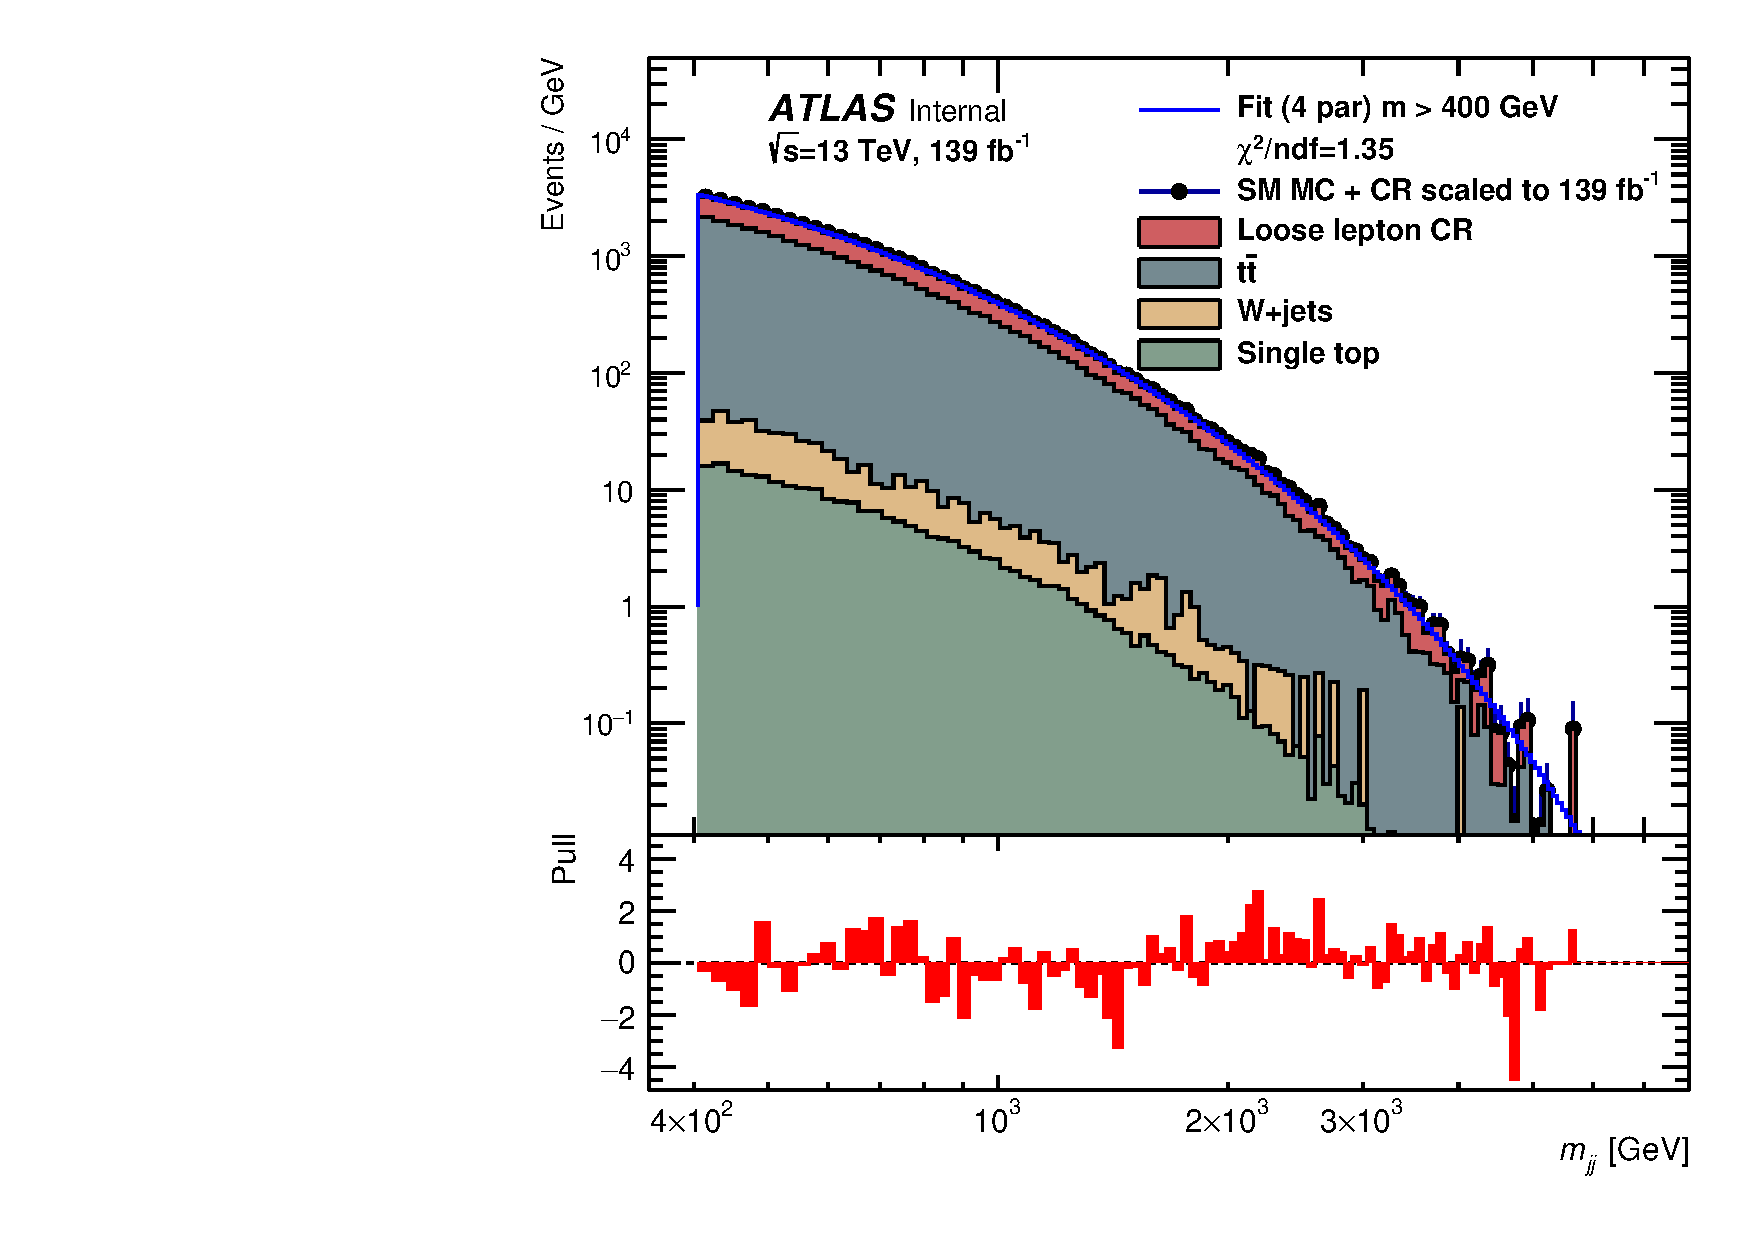
\includegraphics[scale=0.3]{figs/ch6/fit/variable_nosmooth/p4/10PB/output_SMMCplusCR_Mjj_p4.pdf}%
    \caption{\mjj \ using MC+LE-CR, p4}
    \end{subfigure}
    \hfill
    \begin{subfigure}[h]{0.4\linewidth}
    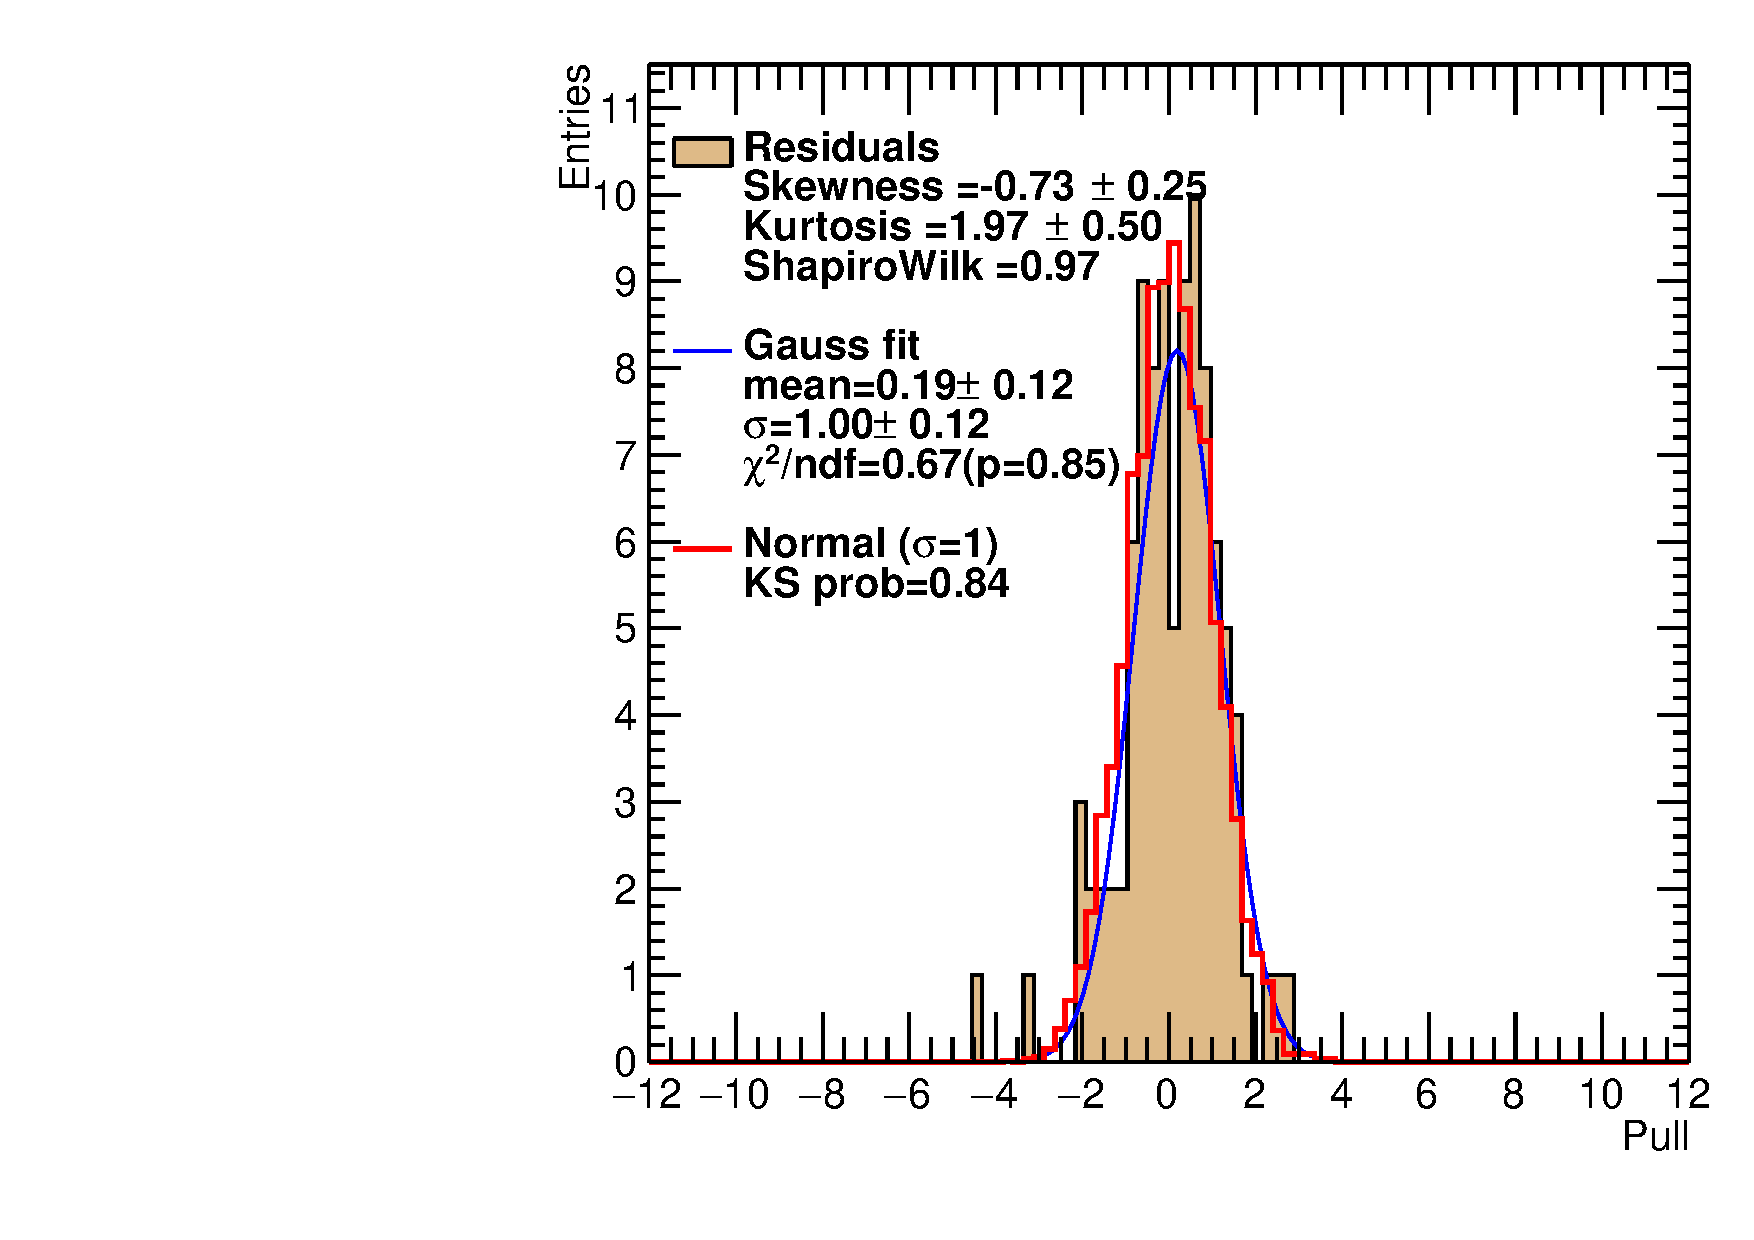
\includegraphics[scale=0.32]{figs/ch6/fit/variable_nosmooth/p4/10PB/pull_SMMCplusCR_Mjj_p4.pdf}%
    \caption{pulls of \mjj \ in p4}
    \end{subfigure}
    \hfill
    \begin{subfigure}[h]{0.38\linewidth}
    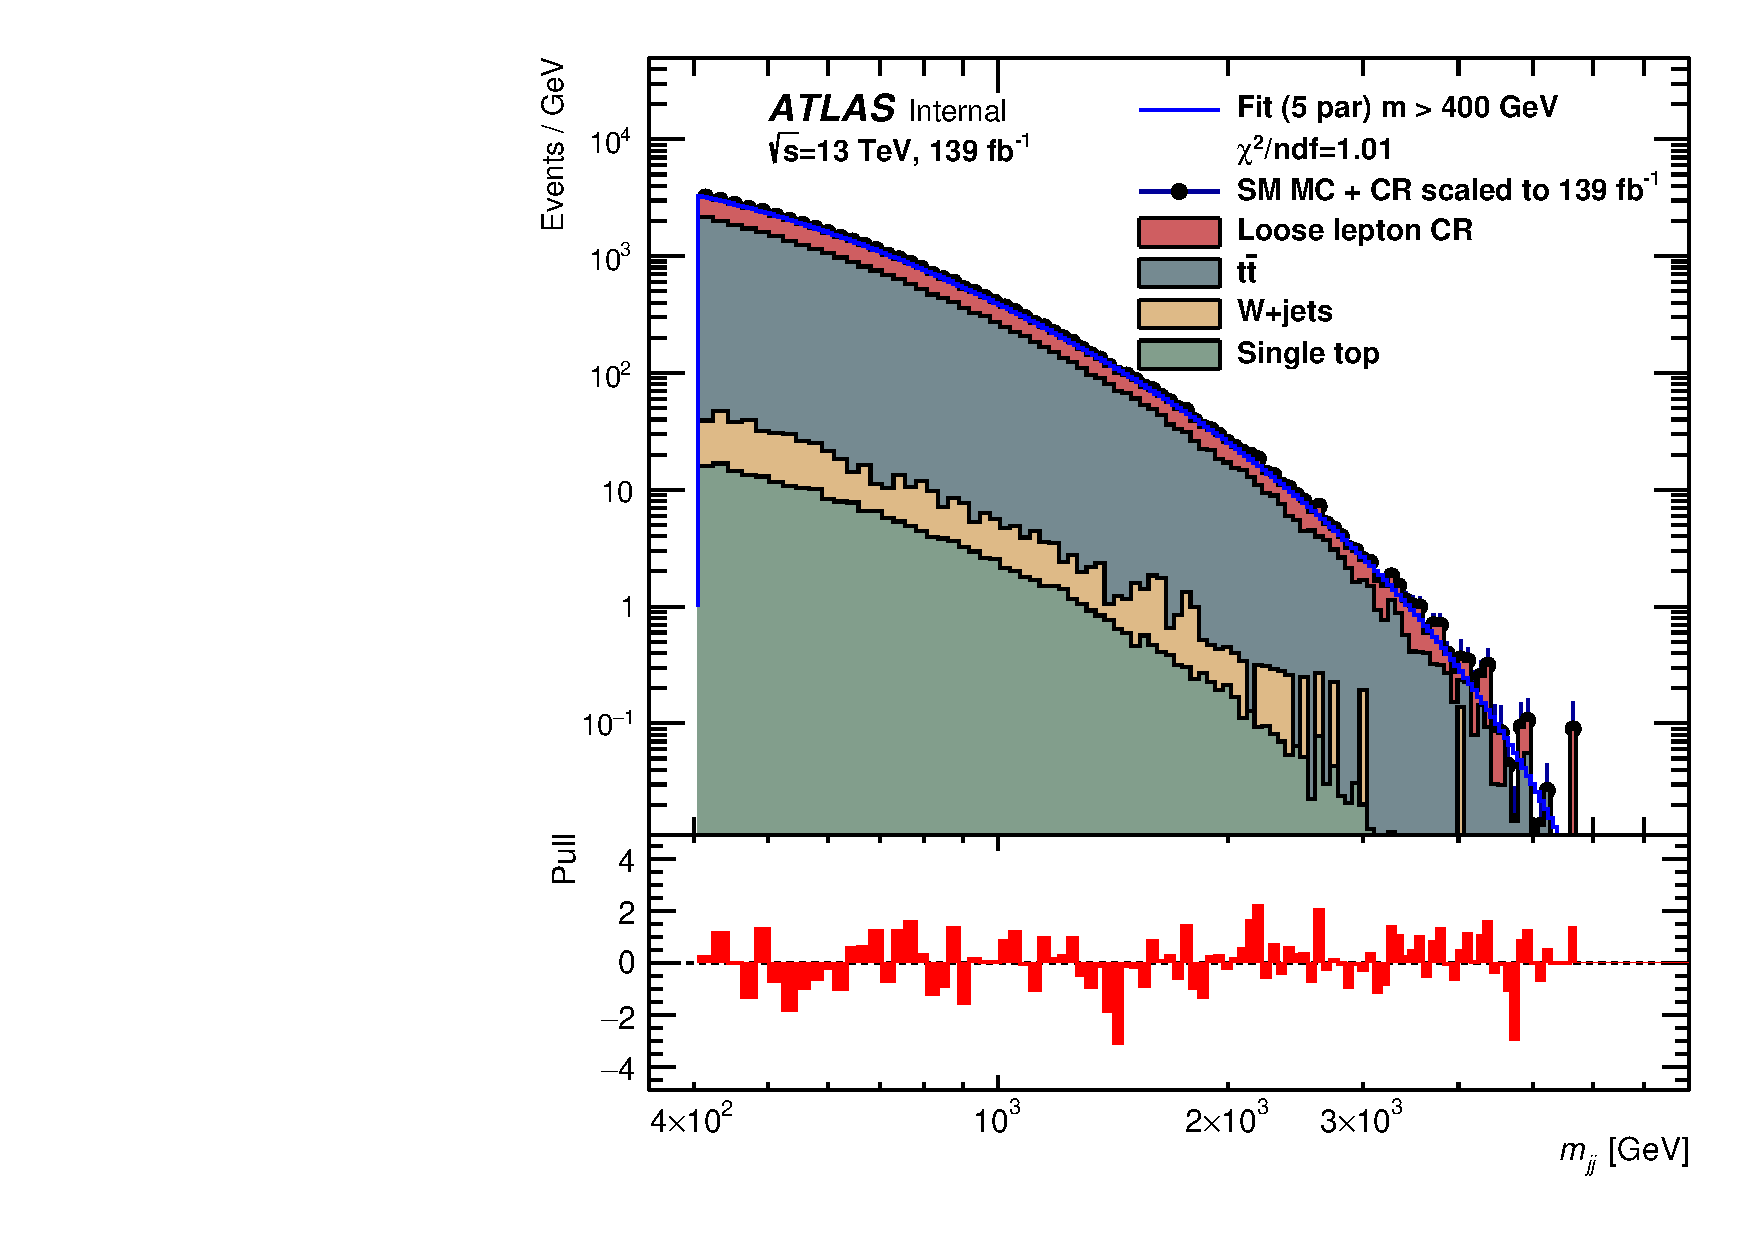
\includegraphics[scale=0.3]{figs/ch6/fit/variable_nosmooth/p5/10PB/output_SMMCplusCR_Mjj_p5.pdf}%
     \caption{\mjj \ using MC+LE-CR, p5}
     \end{subfigure}
     \hfill
    \begin{subfigure}[h]{0.4\linewidth}
    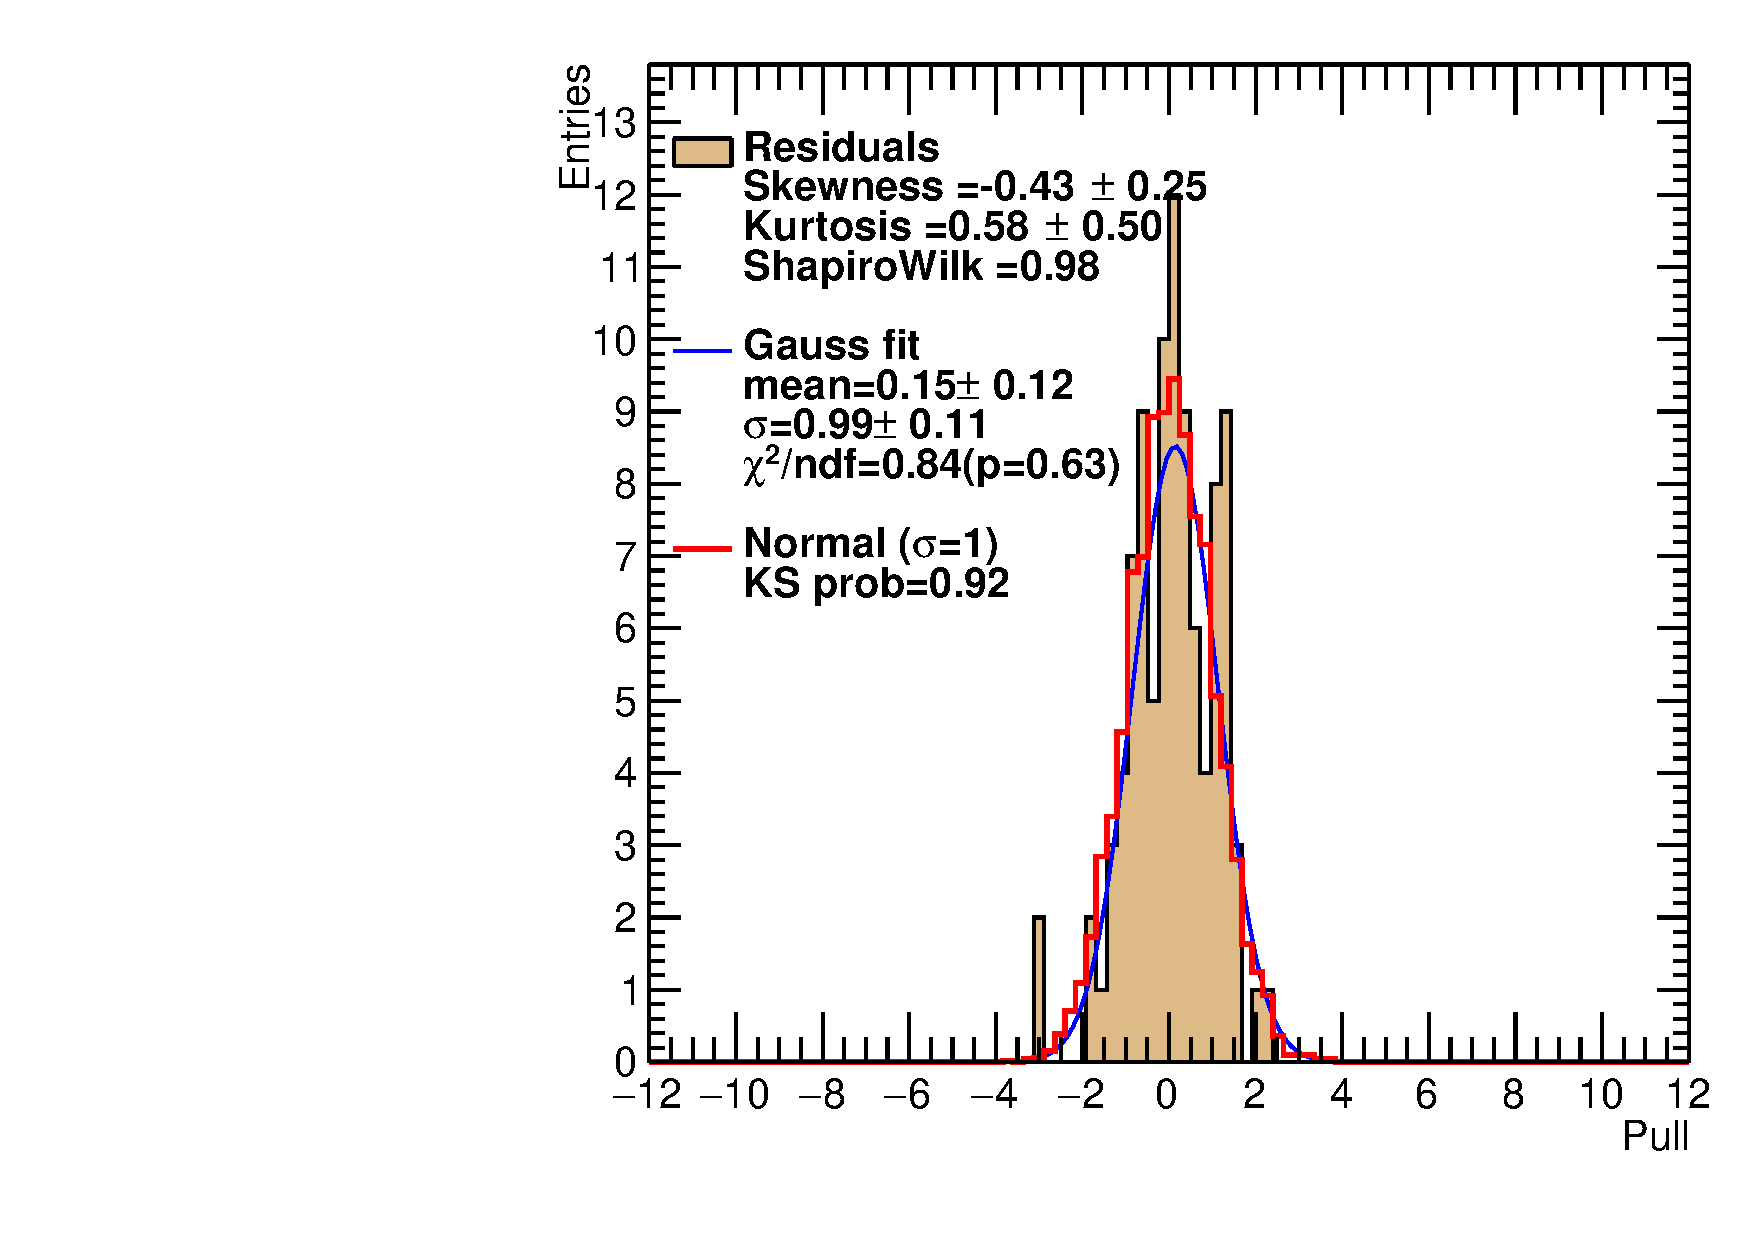
\includegraphics[scale=0.32]{figs/ch6/fit/variable_nosmooth/p5/10PB/pull_SMMCplusCR_Mjj_p5.pdf}%
    \caption{pulls of \mjj \ in p5}
    \end{subfigure}
    \hfill
    \begin{subfigure}[h]{0.38\linewidth}
    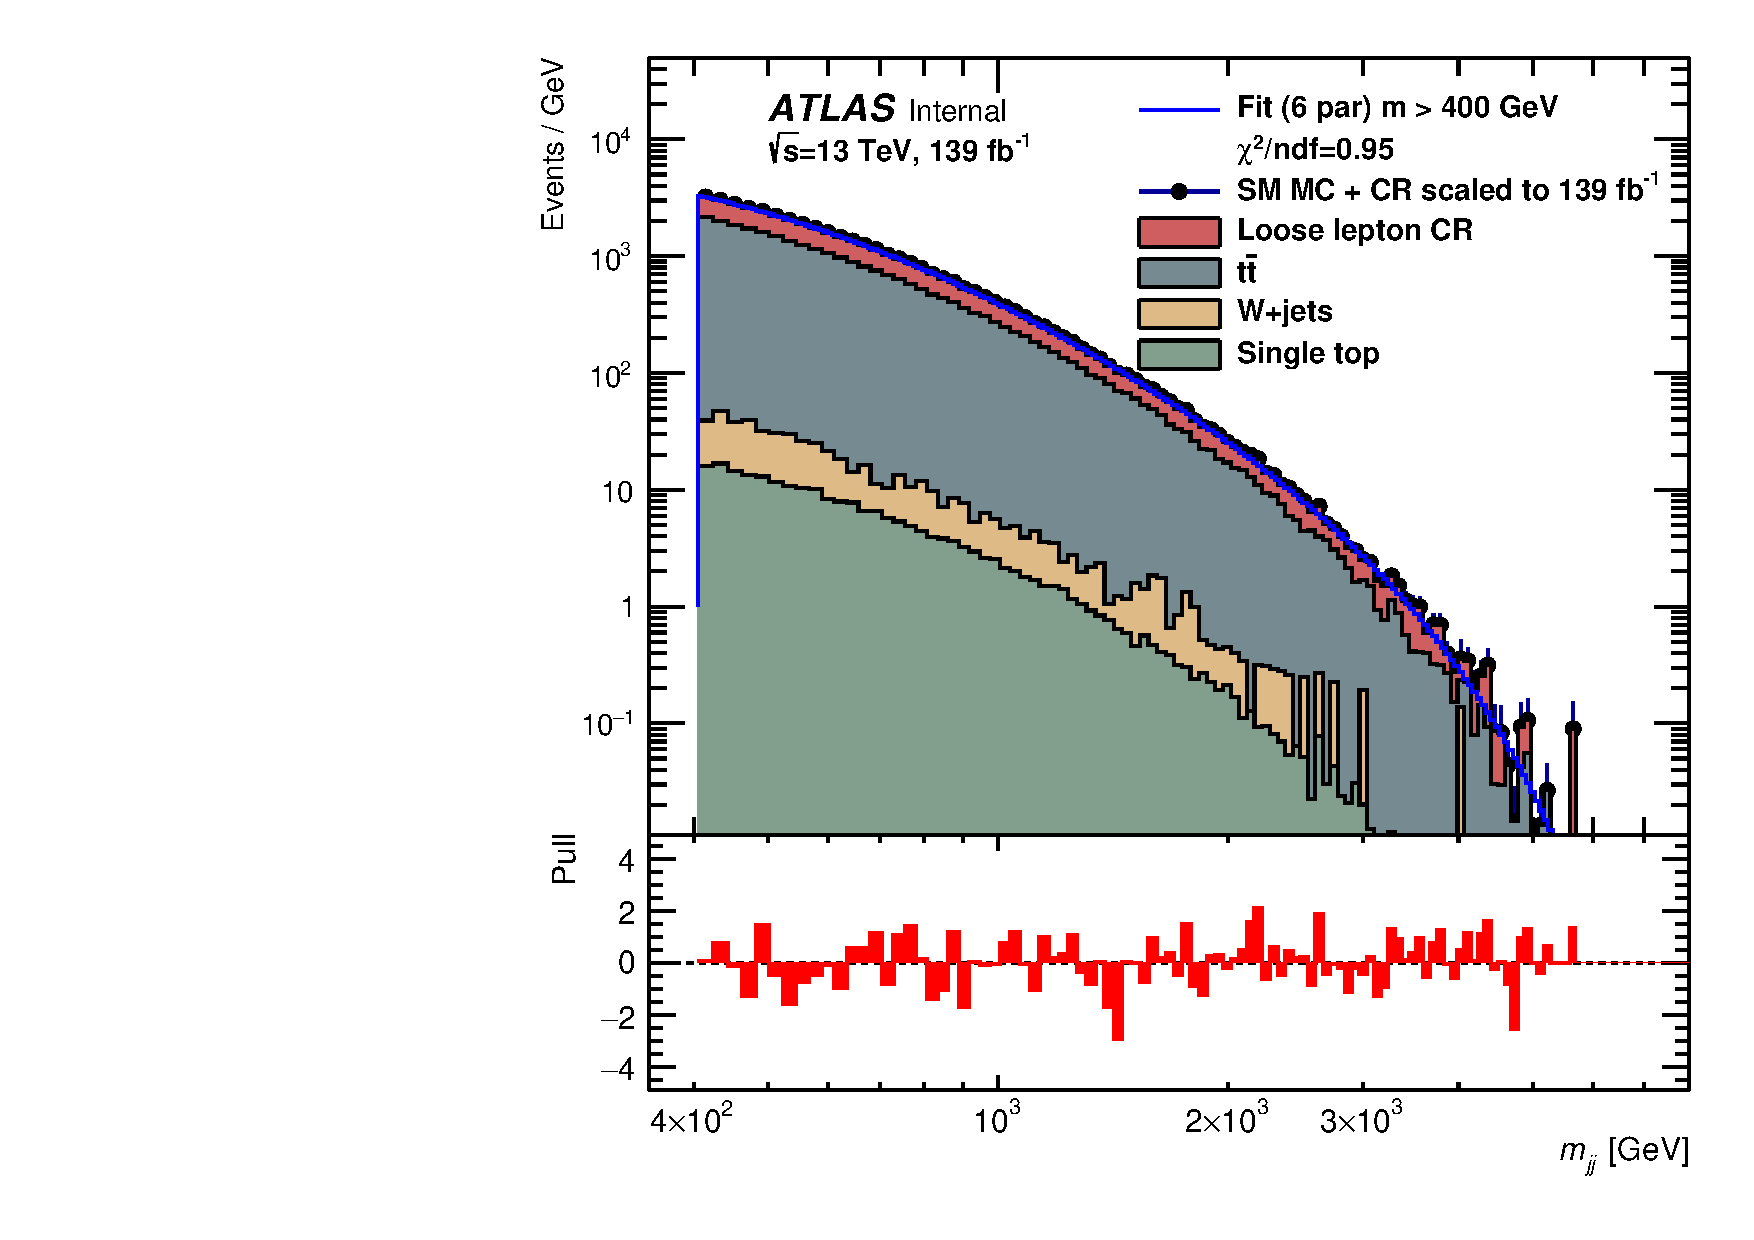
\includegraphics[scale=0.3]{figs/ch6/fit/variable_nosmooth/p6/10PB/output_SMMCplusCR_Mjj_p6.pdf}%
    \caption{\mjj \ using MC+LE-CR, p6}
    \end{subfigure}
    \hfill
    \begin{subfigure}[h]{0.4\linewidth}
    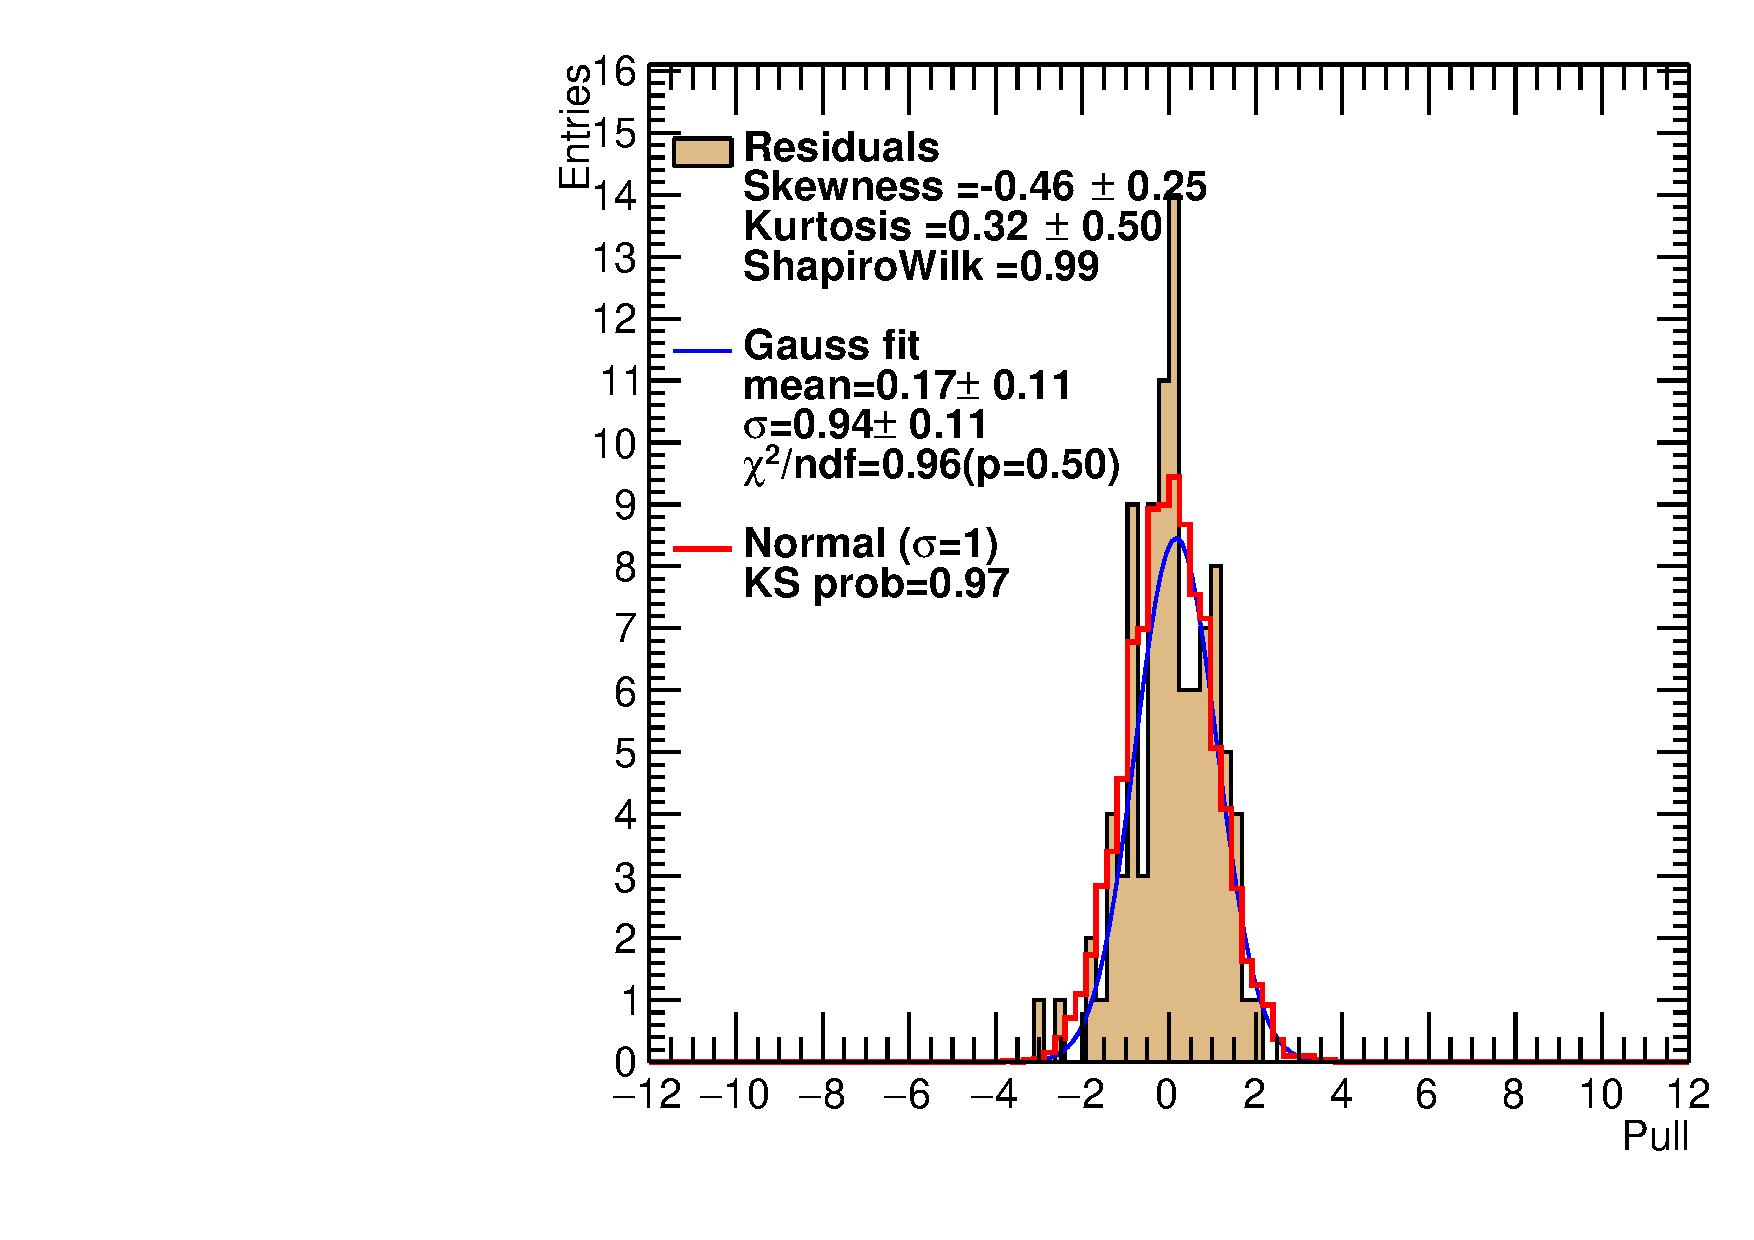
\includegraphics[scale=0.32]{figs/ch6/fit/variable_nosmooth/p6/10PB/pull_SMMCplusCR_Mjj_p6.pdf}%
    \caption{pulls of \mjj \ in p6}
    \end{subfigure}
    \hfill
    \caption{The \mjj \ invariant masses with the p4, p5 and p6 fit functions in the BSM region after the 10 pb AR cut is applied. Pulls shown on the right.}
\label{fig:mjj-fit-pulls}
\end{figure}

\newpage

\begin{figure}[H]
    \centering
    \begin{subfigure}[h]{0.38\linewidth}
    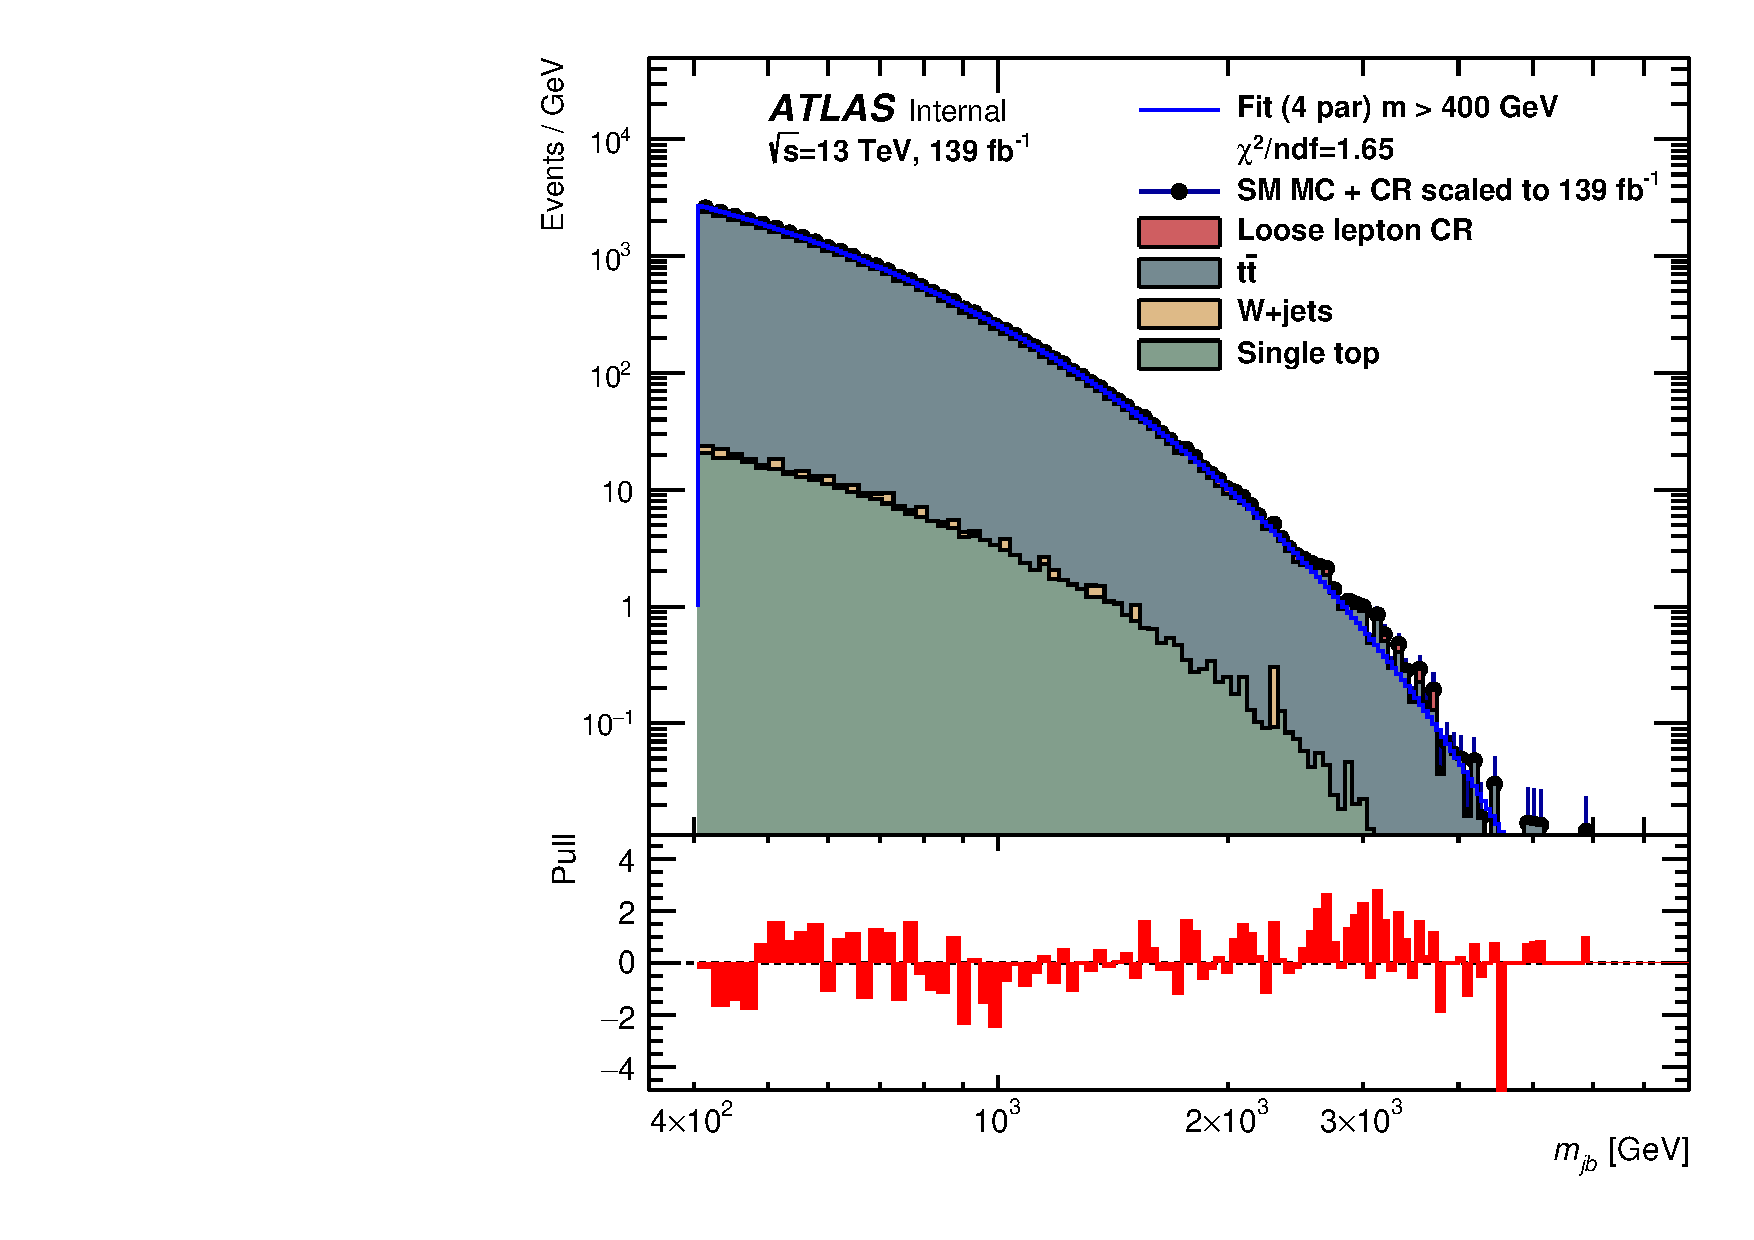
\includegraphics[scale=0.3]{figs/ch6/fit/variable_nosmooth/p4/10PB/output_SMMCplusCR_Mjb_p4.pdf}%
    \caption{\mjb \ using MC+LE-CR, p4}
    \end{subfigure}
    \hfill
    \begin{subfigure}[h]{0.4\linewidth}
    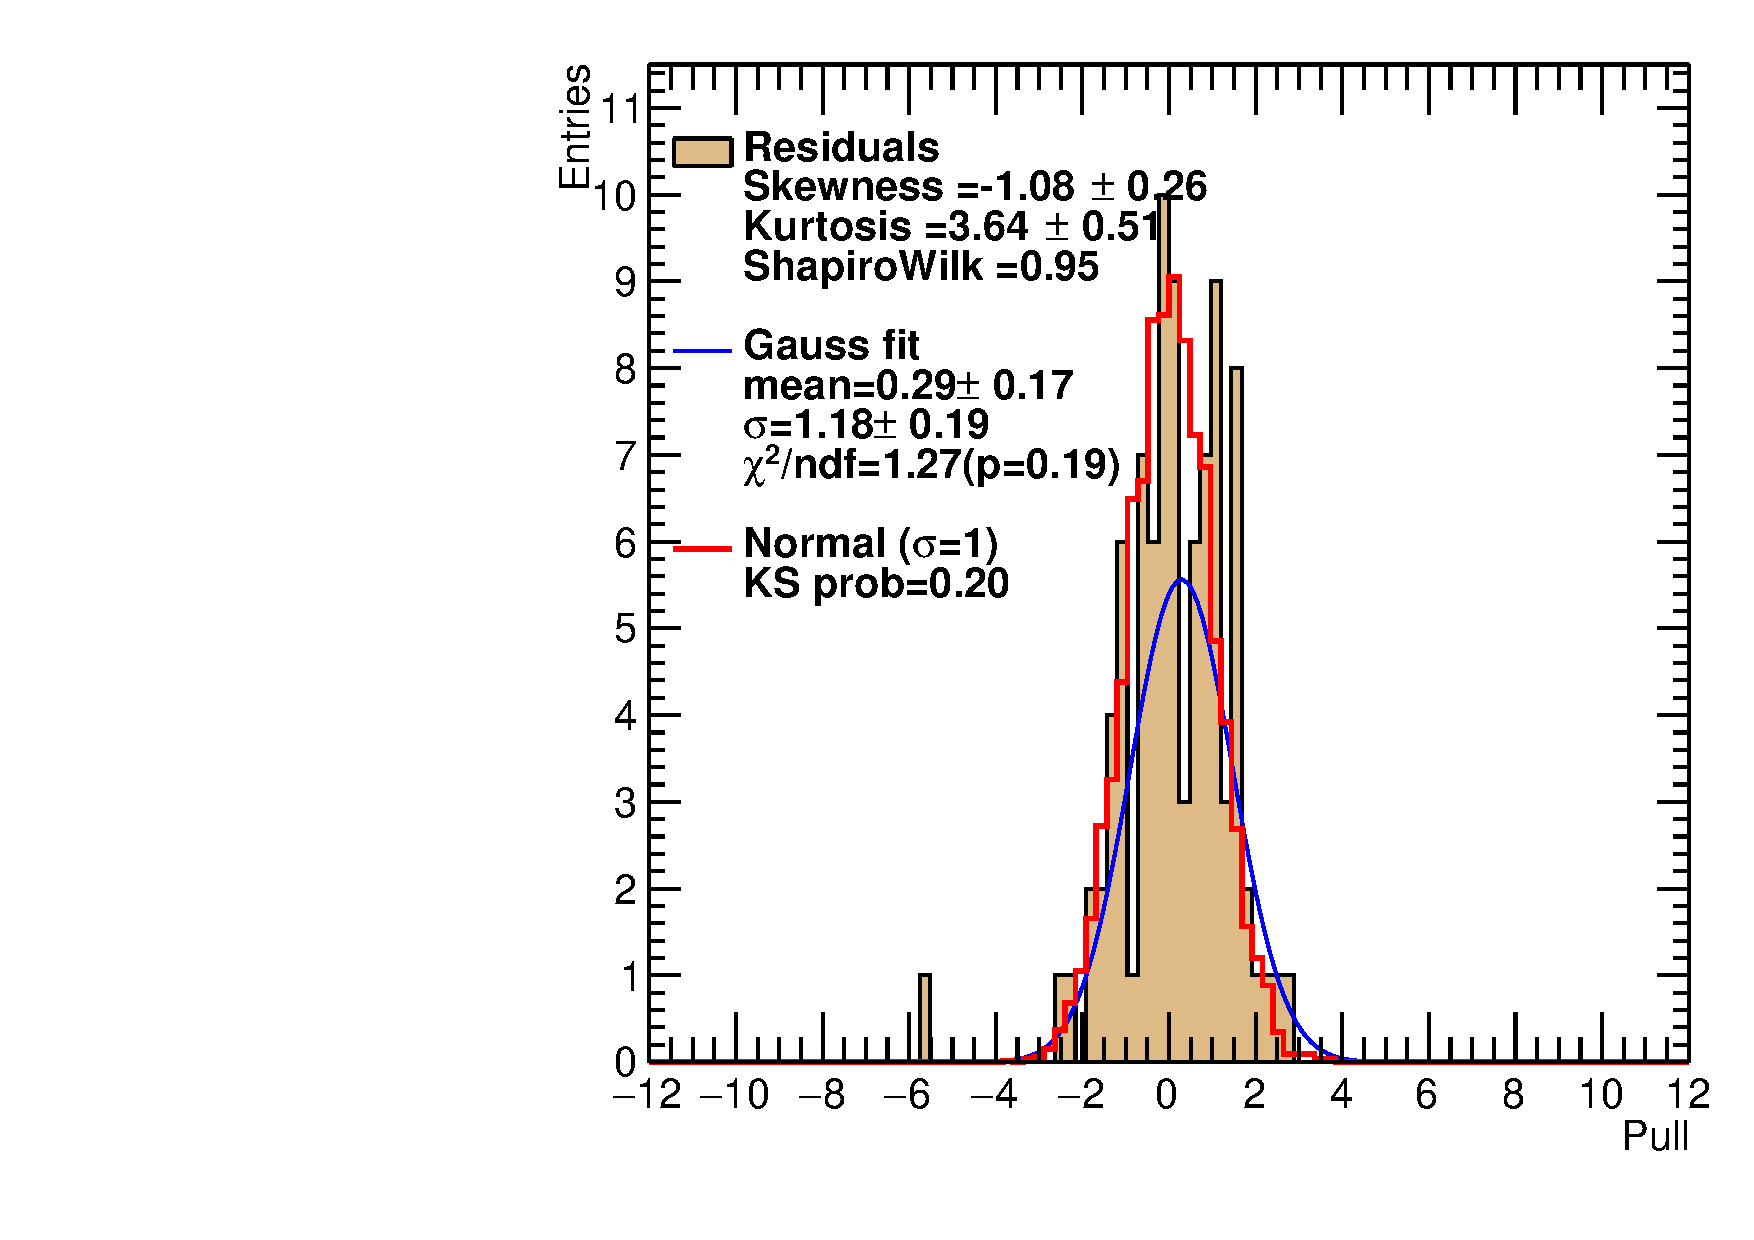
\includegraphics[scale=0.32]{figs/ch6/fit/variable_nosmooth/p4/10PB/pull_SMMCplusCR_Mjb_p4.pdf}%
    \caption{pulls of \mjb \ in p4}
    \end{subfigure}
    \hfill
    \begin{subfigure}[h]{0.38\linewidth}
    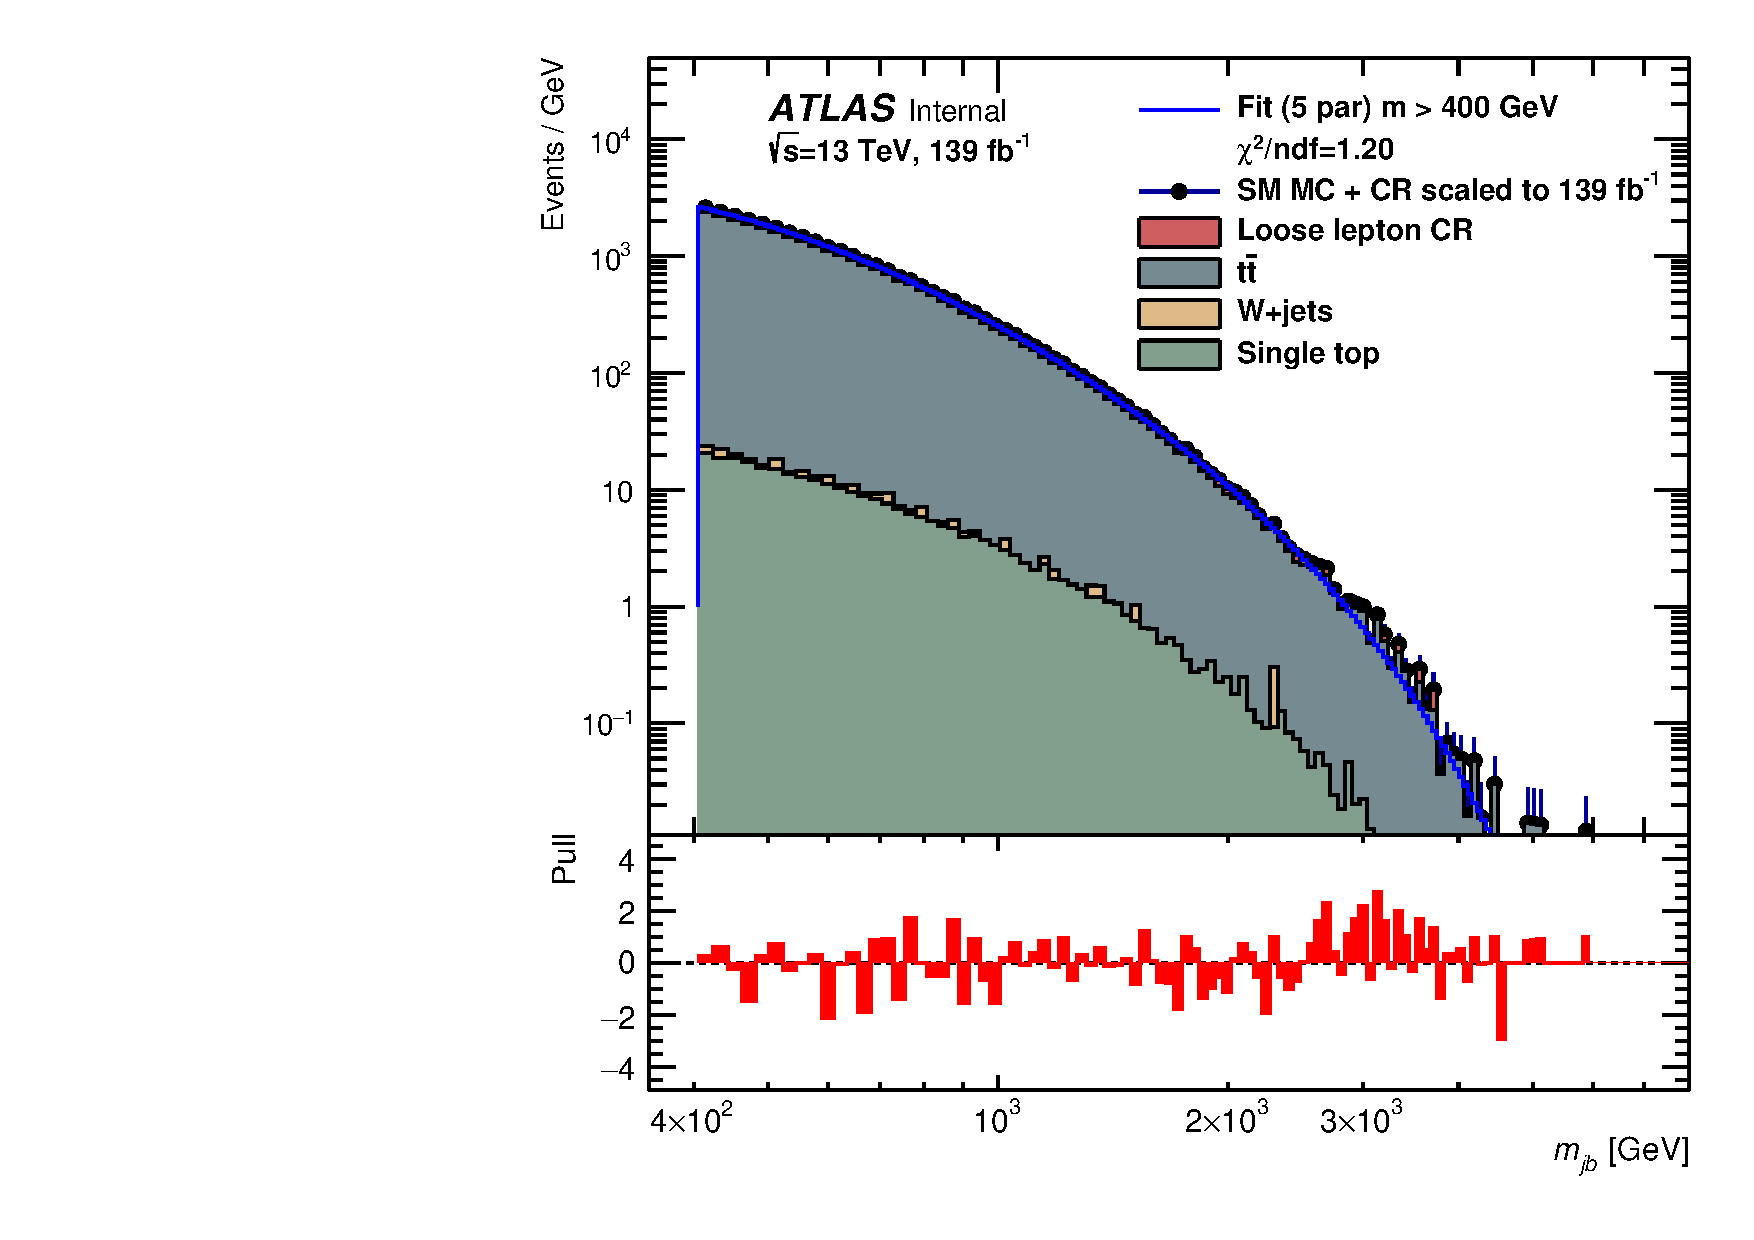
\includegraphics[scale=0.3]{figs/ch6/fit/variable_nosmooth/p5/10PB/output_SMMCplusCR_Mjb_p5.pdf}%
     \caption{\mjb \ using MC+LE-CR, p5}
     \end{subfigure}
     \hfill
    \begin{subfigure}[h]{0.4\linewidth}
    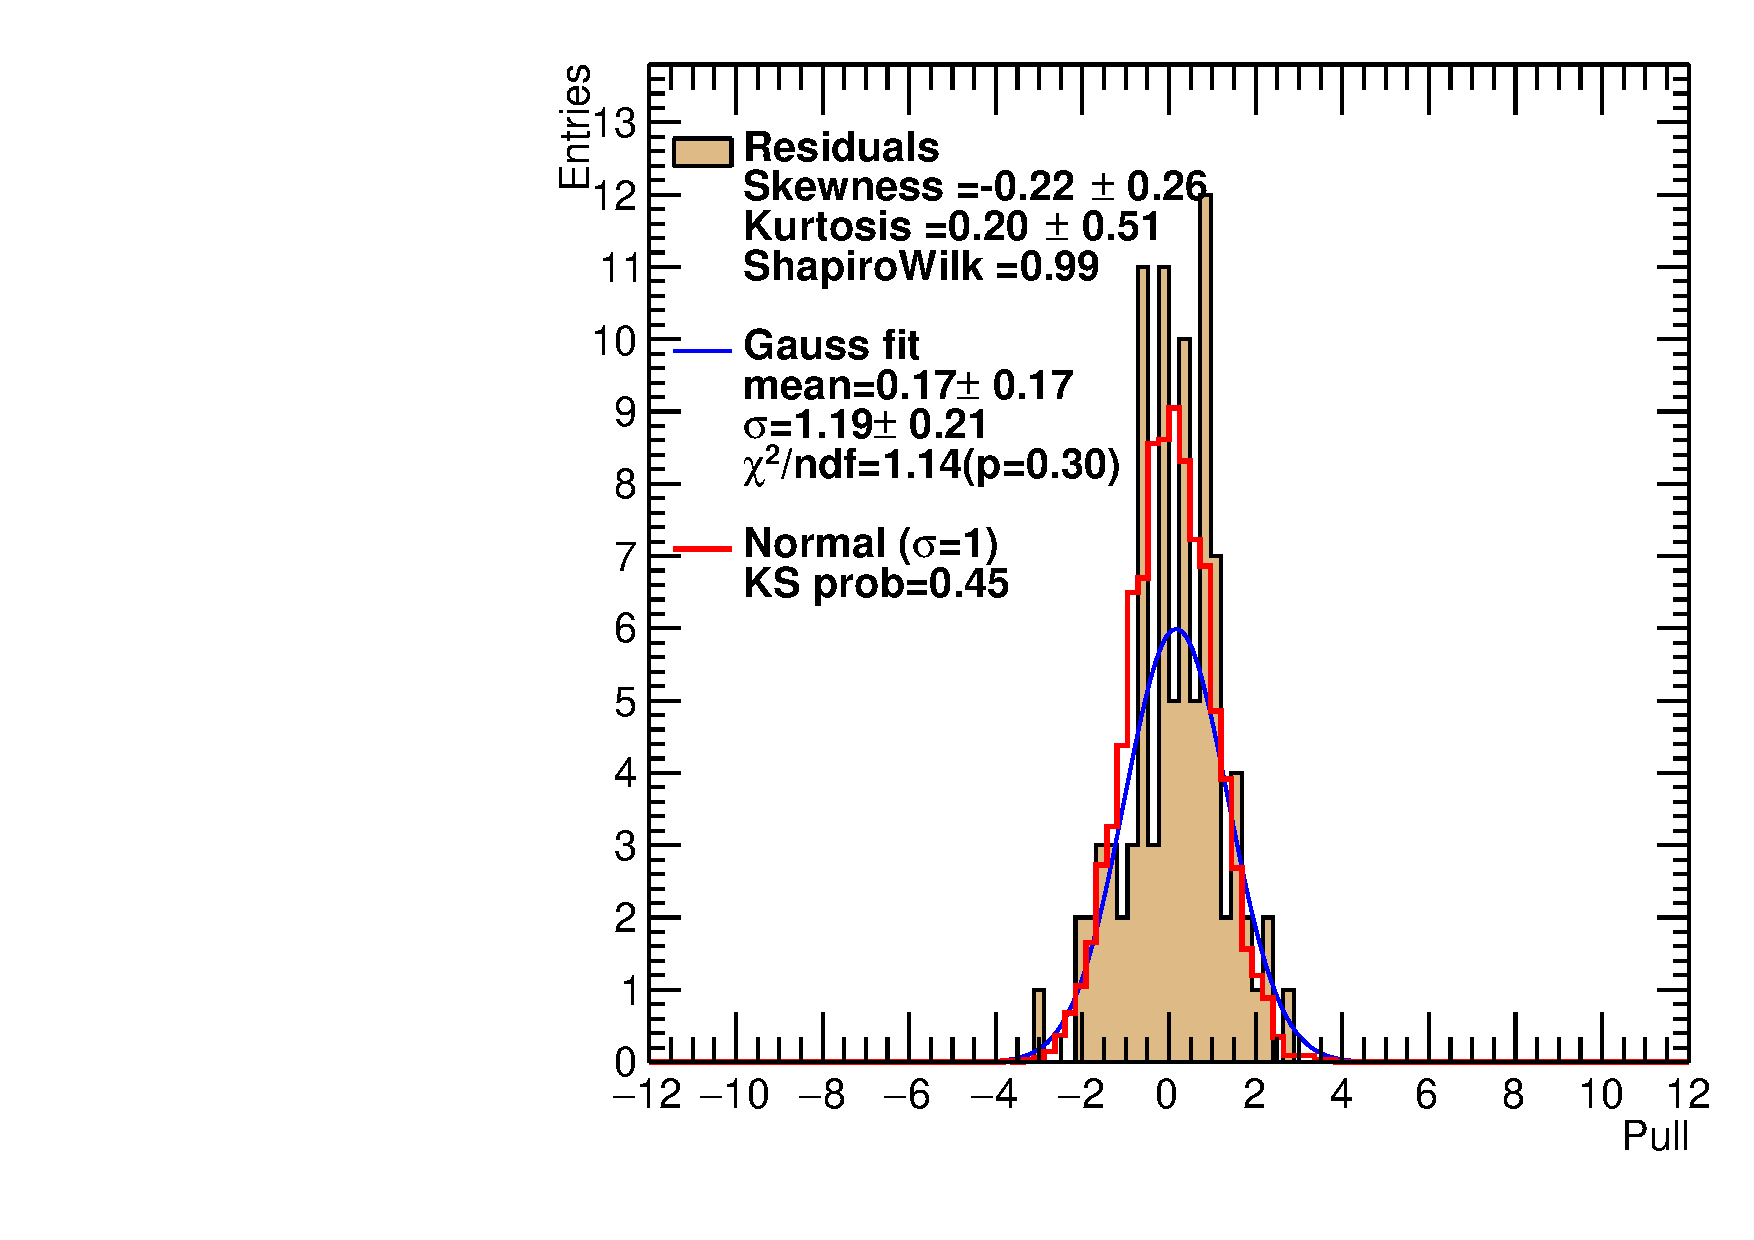
\includegraphics[scale=0.32]{figs/ch6/fit/variable_nosmooth/p5/10PB/pull_SMMCplusCR_Mjb_p5.pdf}%
    \caption{pulls of \mjb \ in p5}
    \end{subfigure}
    \hfill
    \begin{subfigure}[h]{0.38\linewidth}
    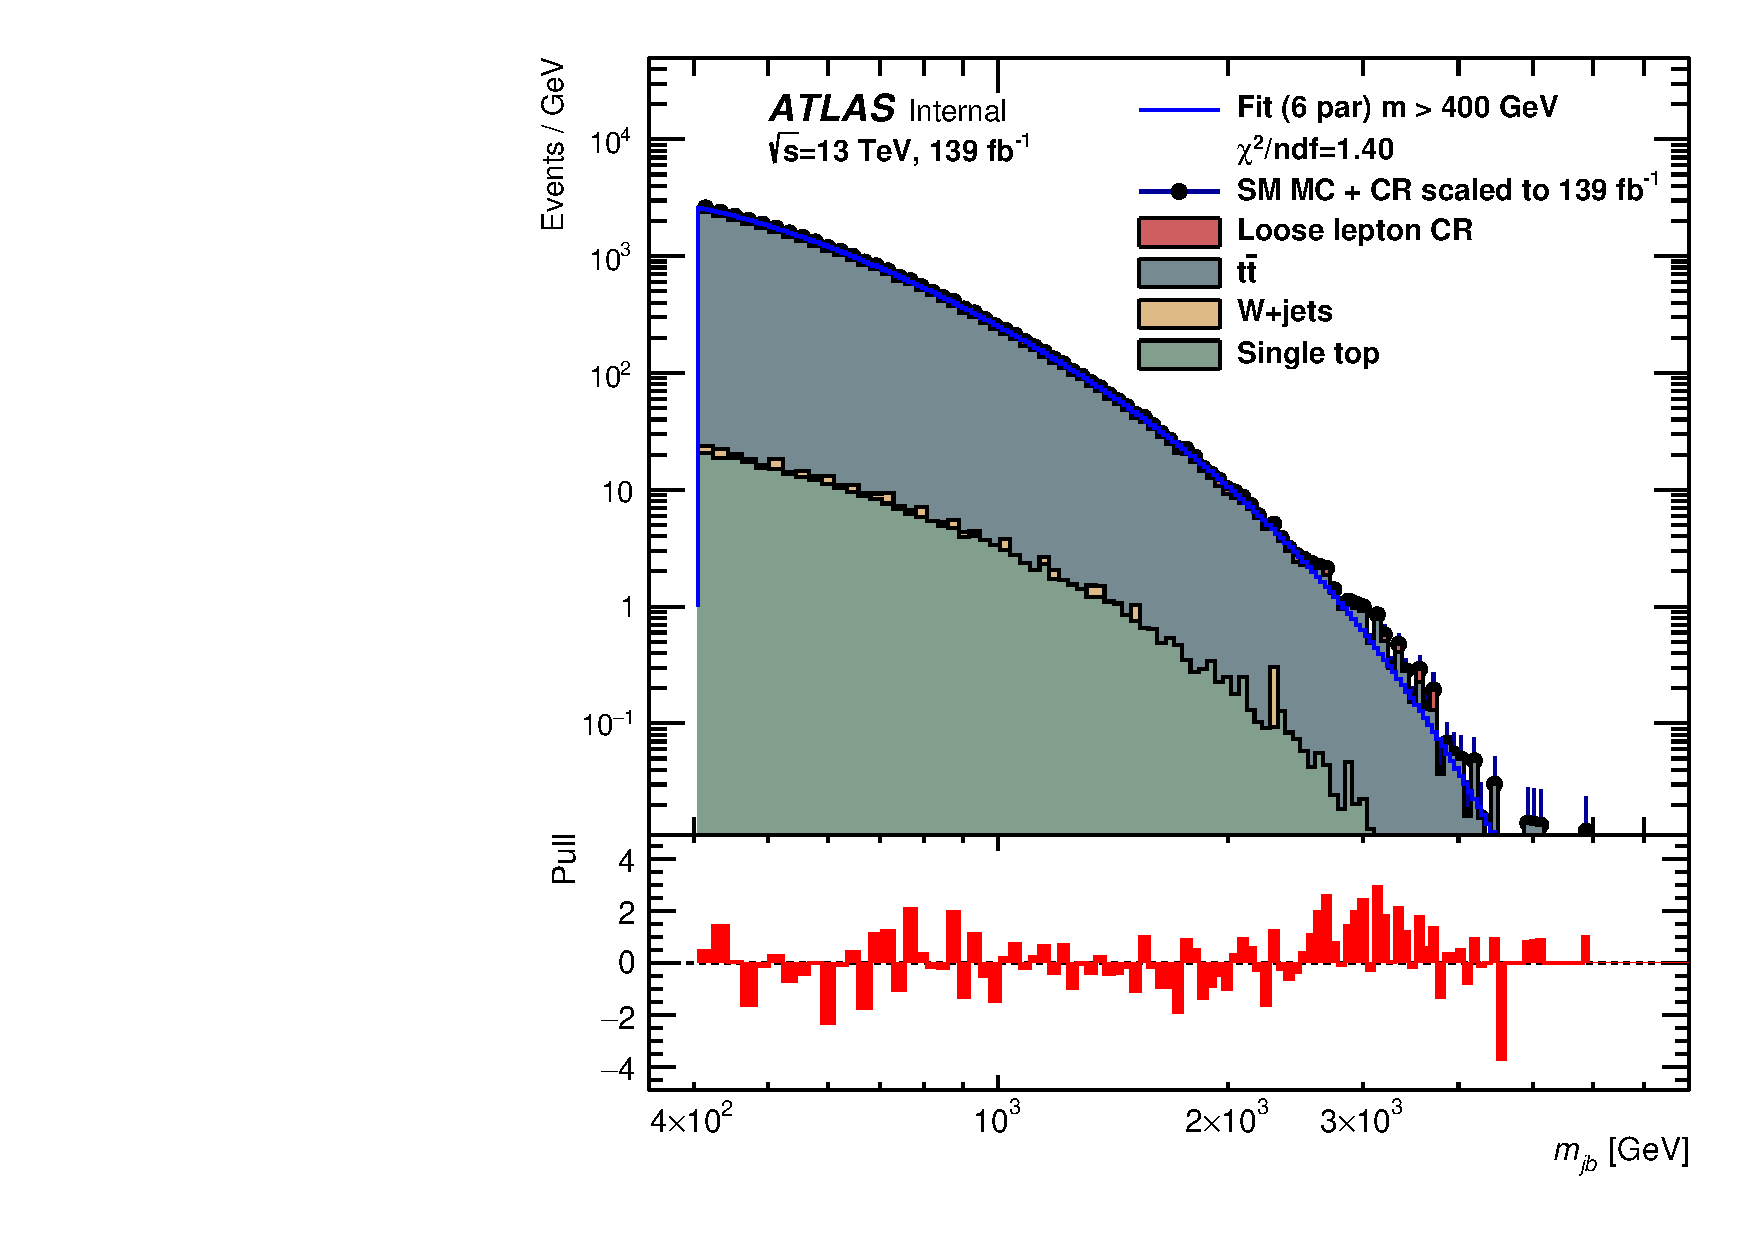
\includegraphics[scale=0.3]{figs/ch6/fit/variable_nosmooth/p6/10PB/output_SMMCplusCR_Mjb_p6.pdf}%
    \caption{\mjb \ using MC+LE-CR, p6}
    \end{subfigure}
    \hfill
    \begin{subfigure}[h]{0.4\linewidth}
    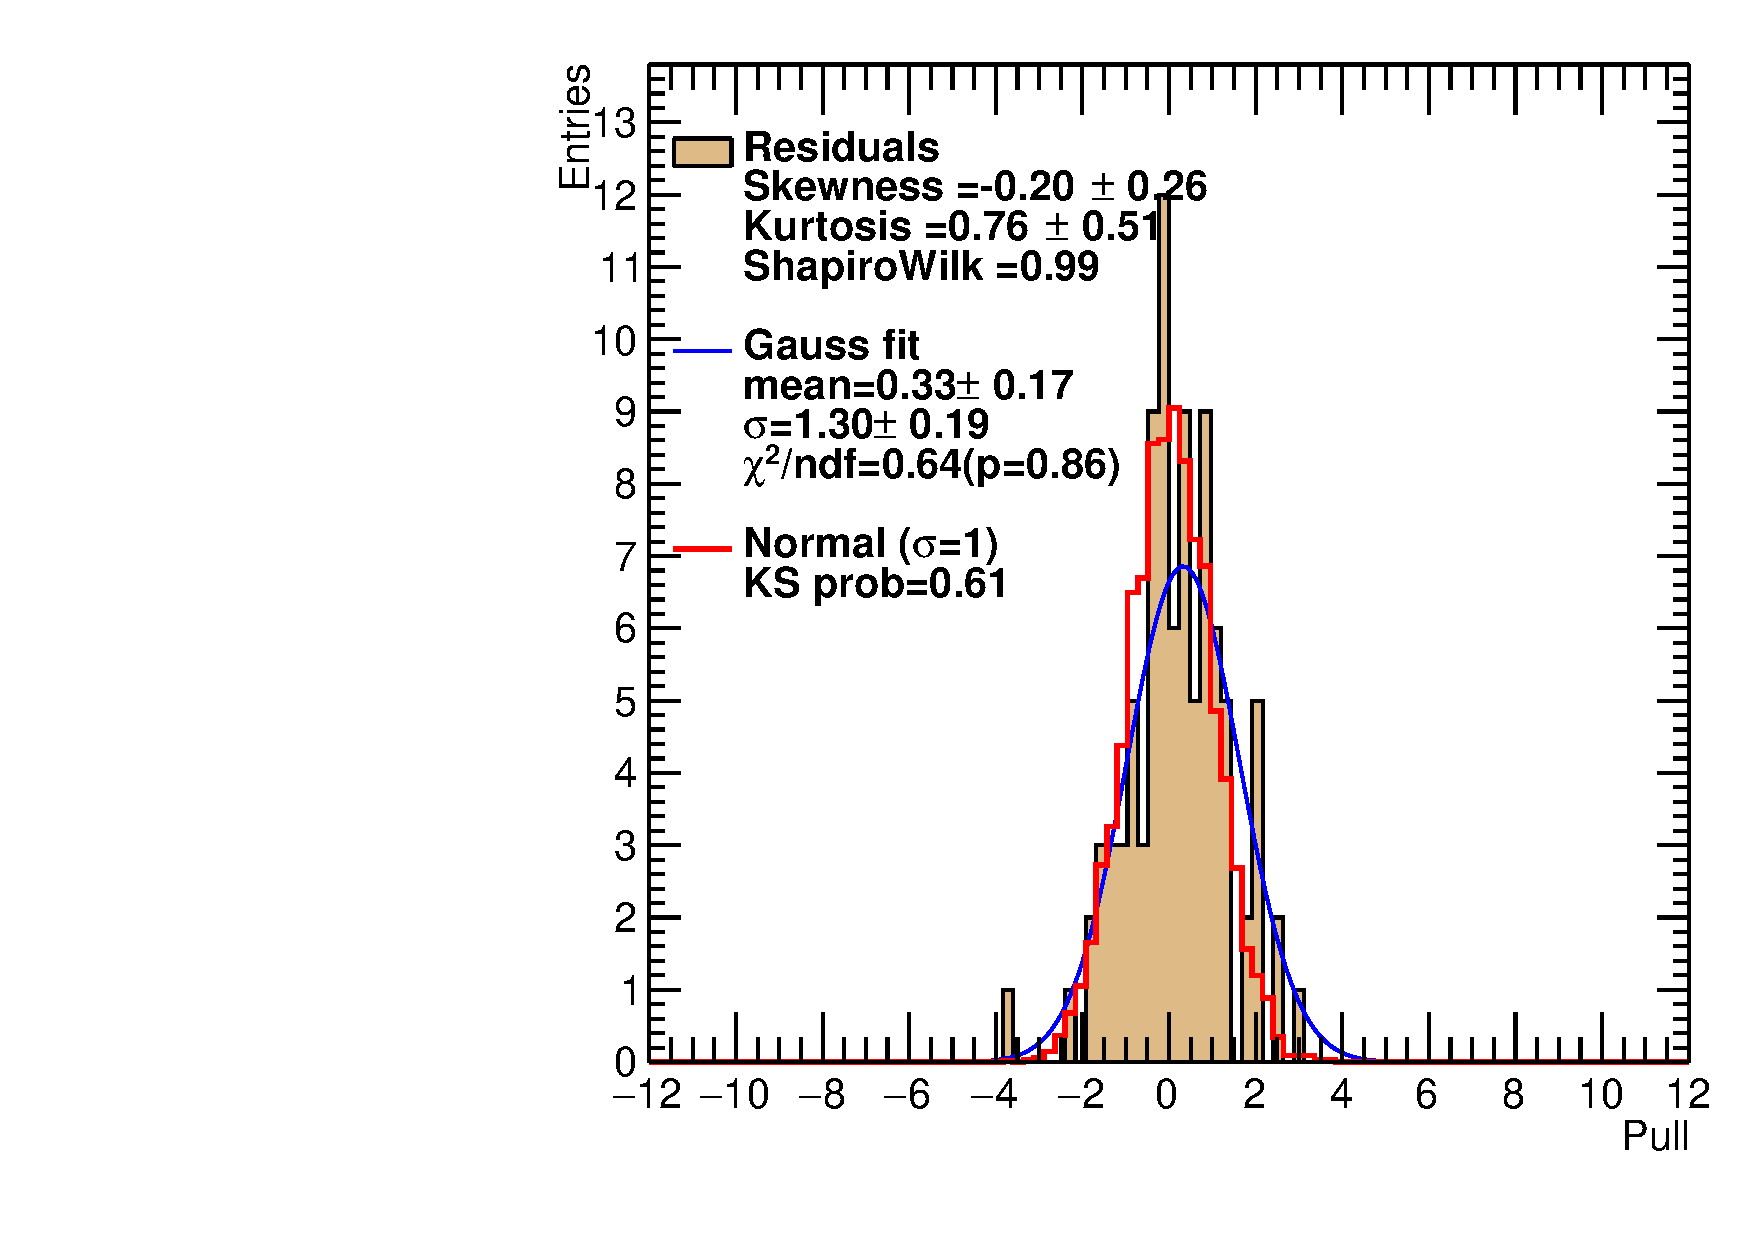
\includegraphics[scale=0.32]{figs/ch6/fit/variable_nosmooth/p6/10PB/pull_SMMCplusCR_Mjb_p6.pdf}%
    \caption{pulls of \mjb \ in p6}
    \end{subfigure}
    \hfill
    \caption{The \mjb \ invariant masses with the p4, p5 and p6 fit functions in the BSM region after the 10 pb AR cut is applied. Pulls shown on the right.}
\label{fig:mjb-fit-pulls}
\end{figure}

\newpage

\begin{figure}[H]
    \centering
    \begin{subfigure}[h]{0.38\linewidth}
    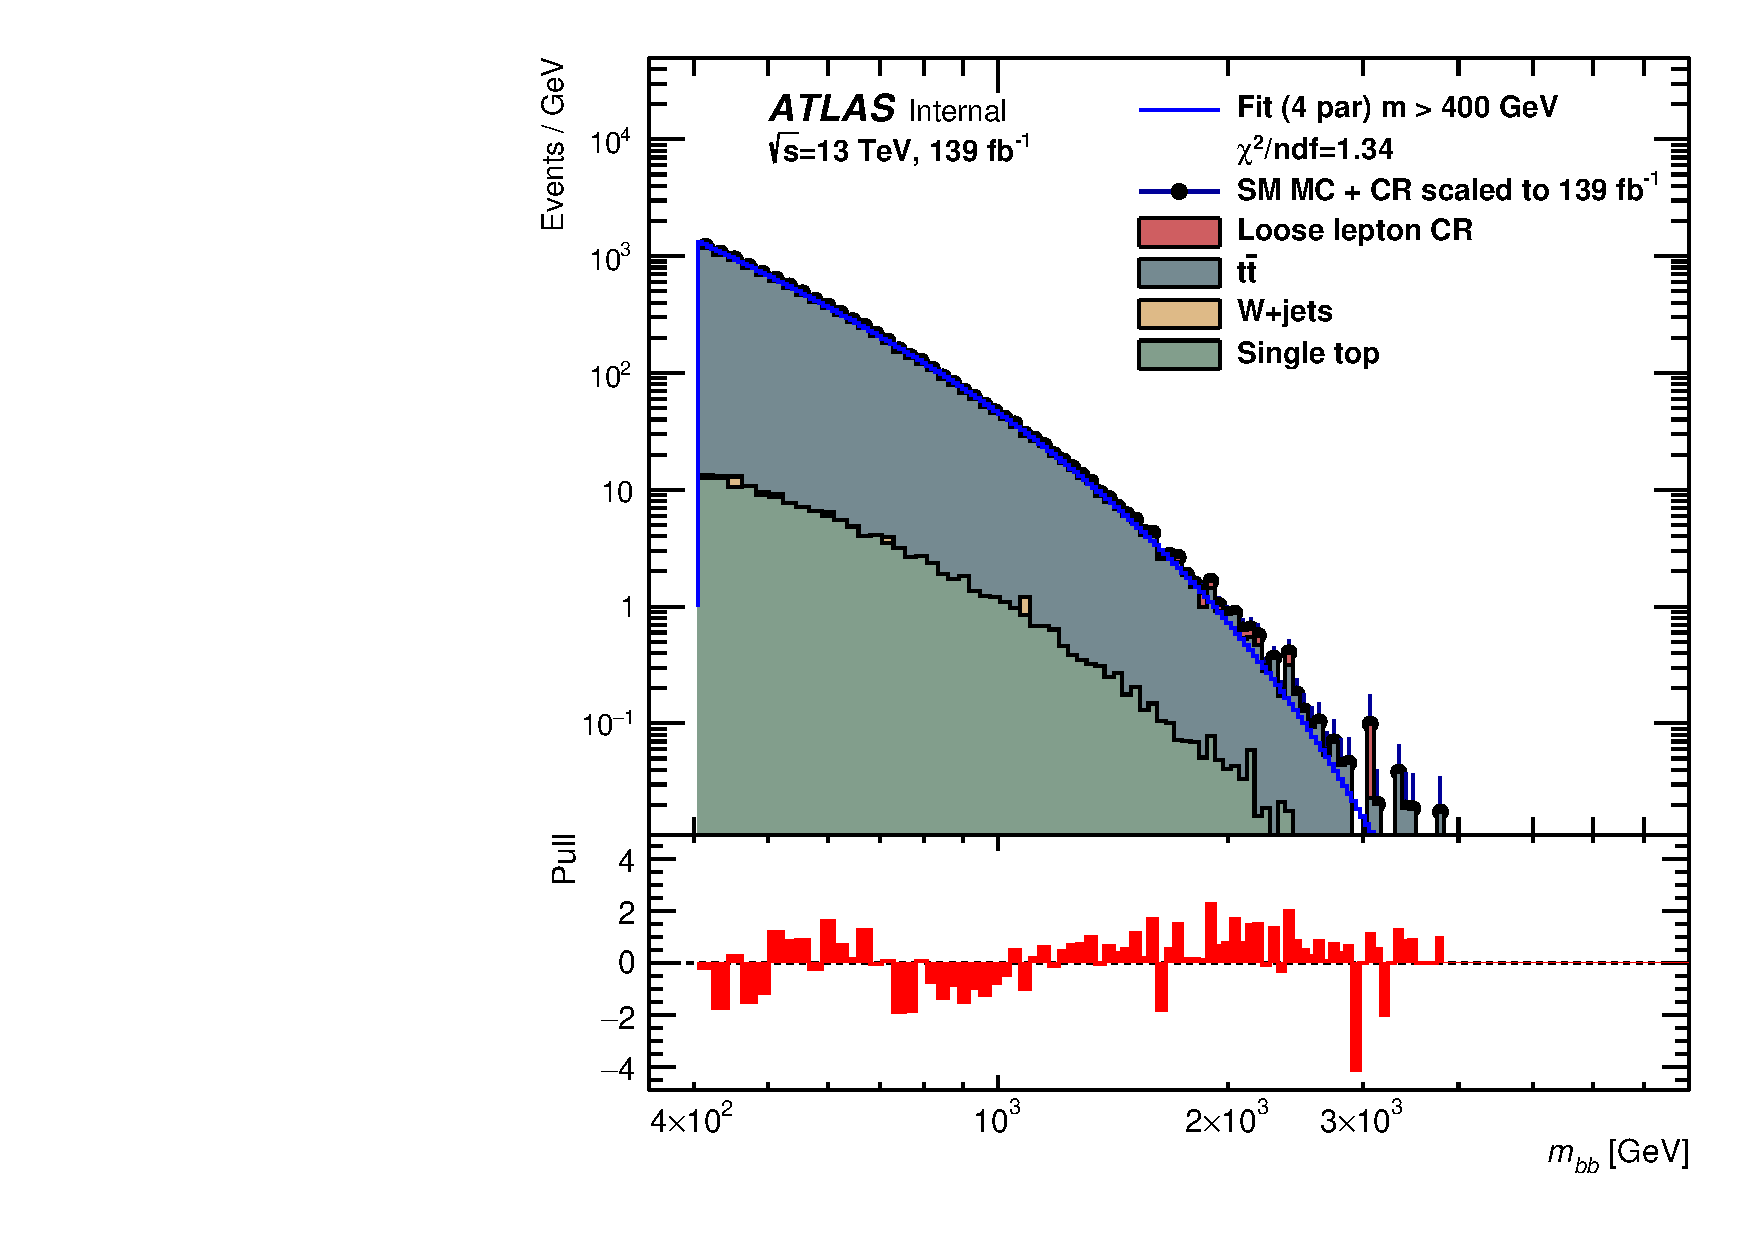
\includegraphics[scale=0.3]{figs/ch6/fit/variable_nosmooth/p4/10PB/output_SMMCplusCR_Mbb_p4.pdf}%
    \caption{\mbb \ using MC+LE-CR, p4}
    \end{subfigure}
    \hfill
    \begin{subfigure}[h]{0.4\linewidth}
    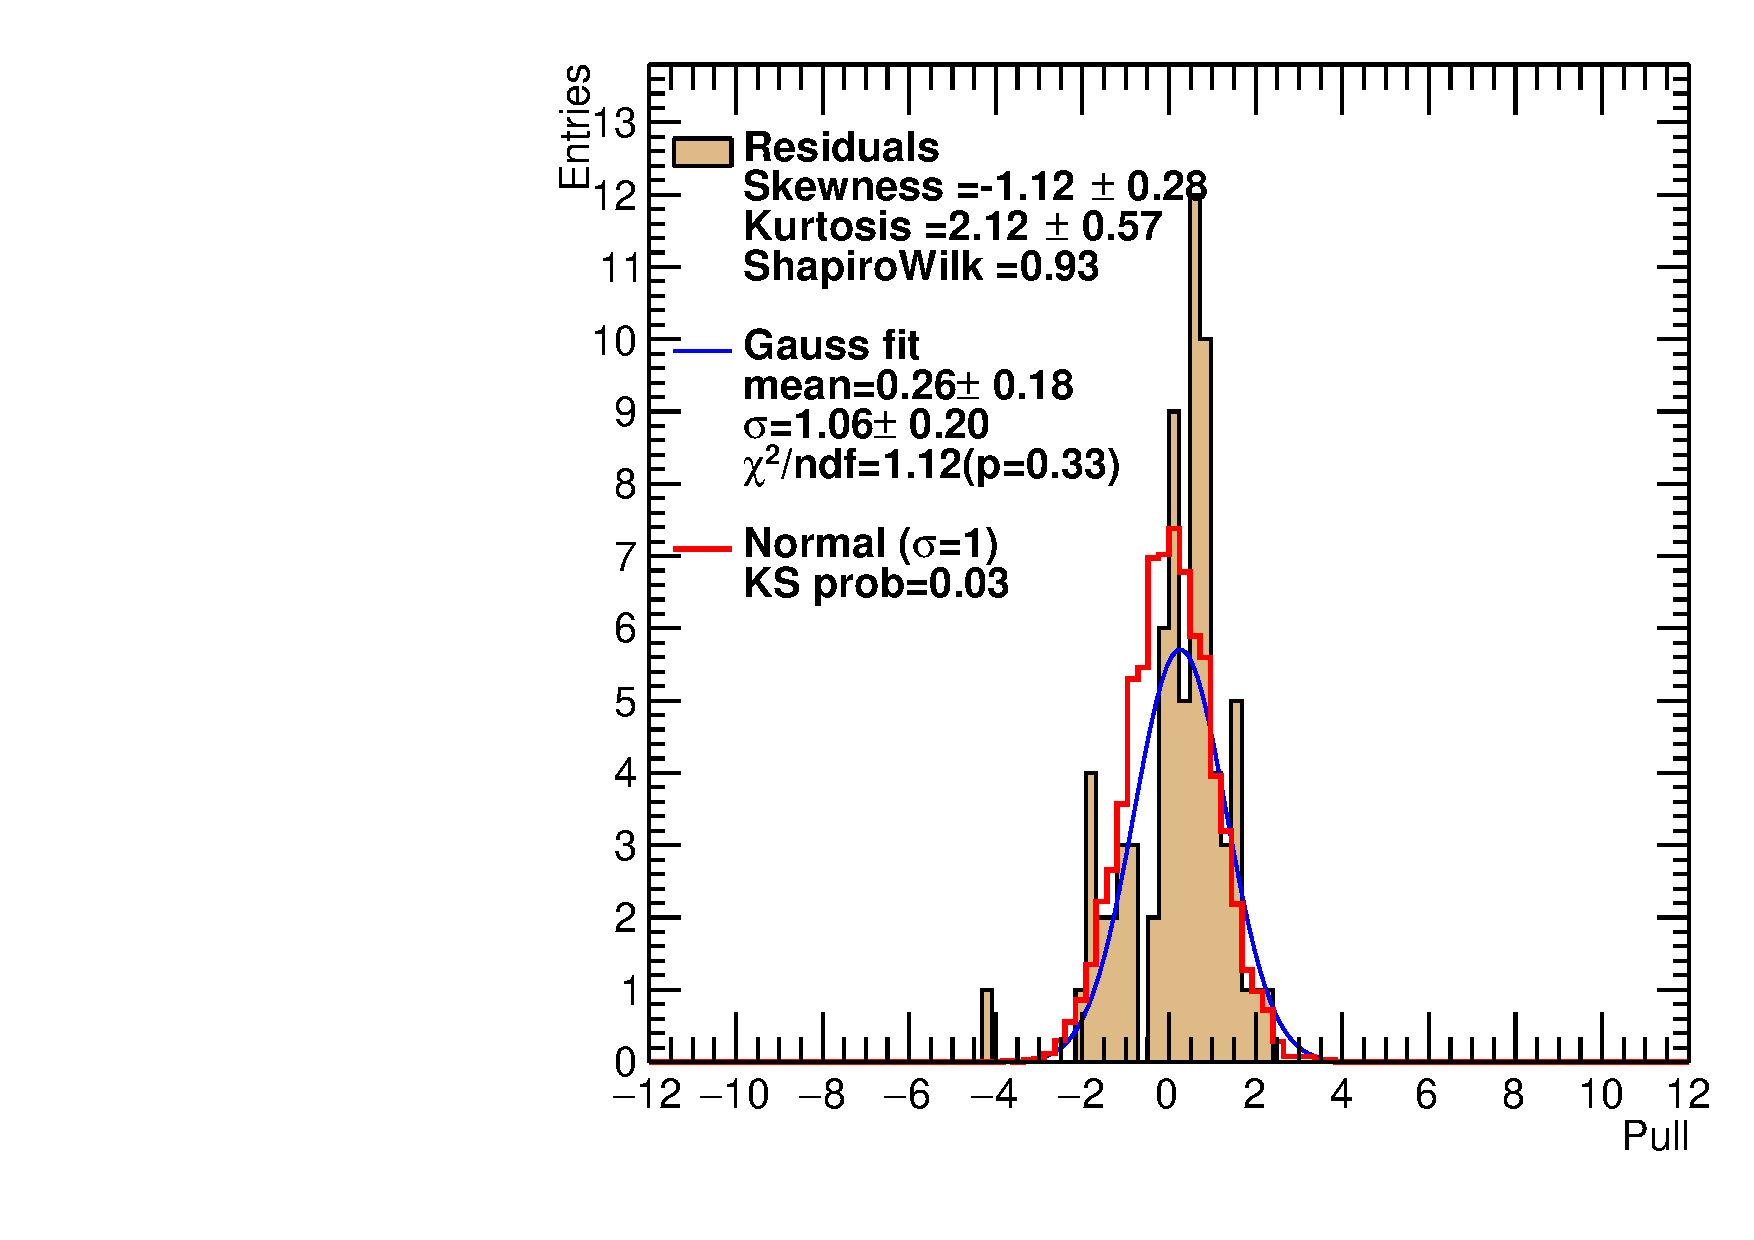
\includegraphics[scale=0.32]{figs/ch6/fit/variable_nosmooth/p4/10PB/pull_SMMCplusCR_Mbb_p4.pdf}%
    \caption{pulls of \mbb \ in p4}
    \end{subfigure}
    \hfill
    \begin{subfigure}[h]{0.38\linewidth}
    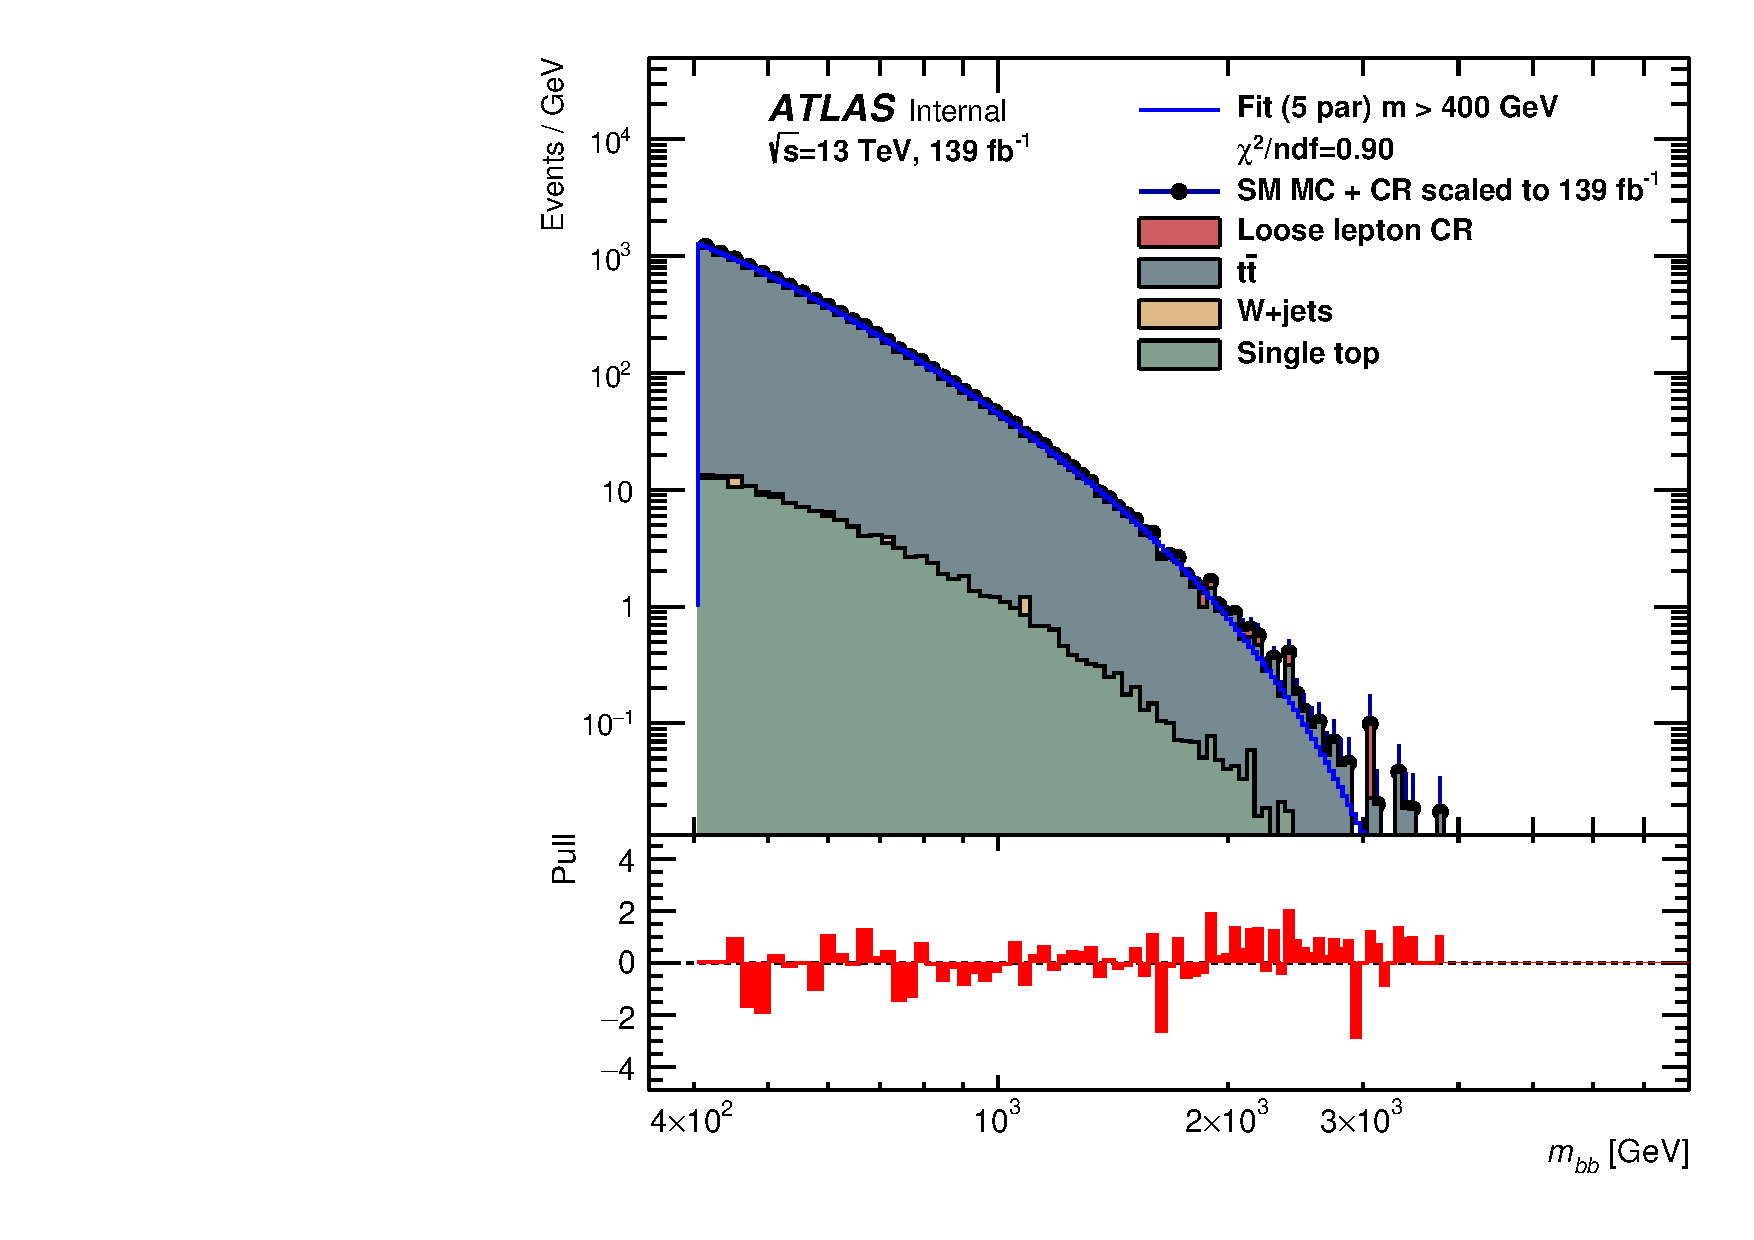
\includegraphics[scale=0.3]{figs/ch6/fit/variable_nosmooth/p5/10PB/output_SMMCplusCR_Mbb_p5.pdf}%
     \caption{\mbb \ using MC+LE-CR, p5}
     \end{subfigure}
     \hfill
    \begin{subfigure}[h]{0.4\linewidth}
    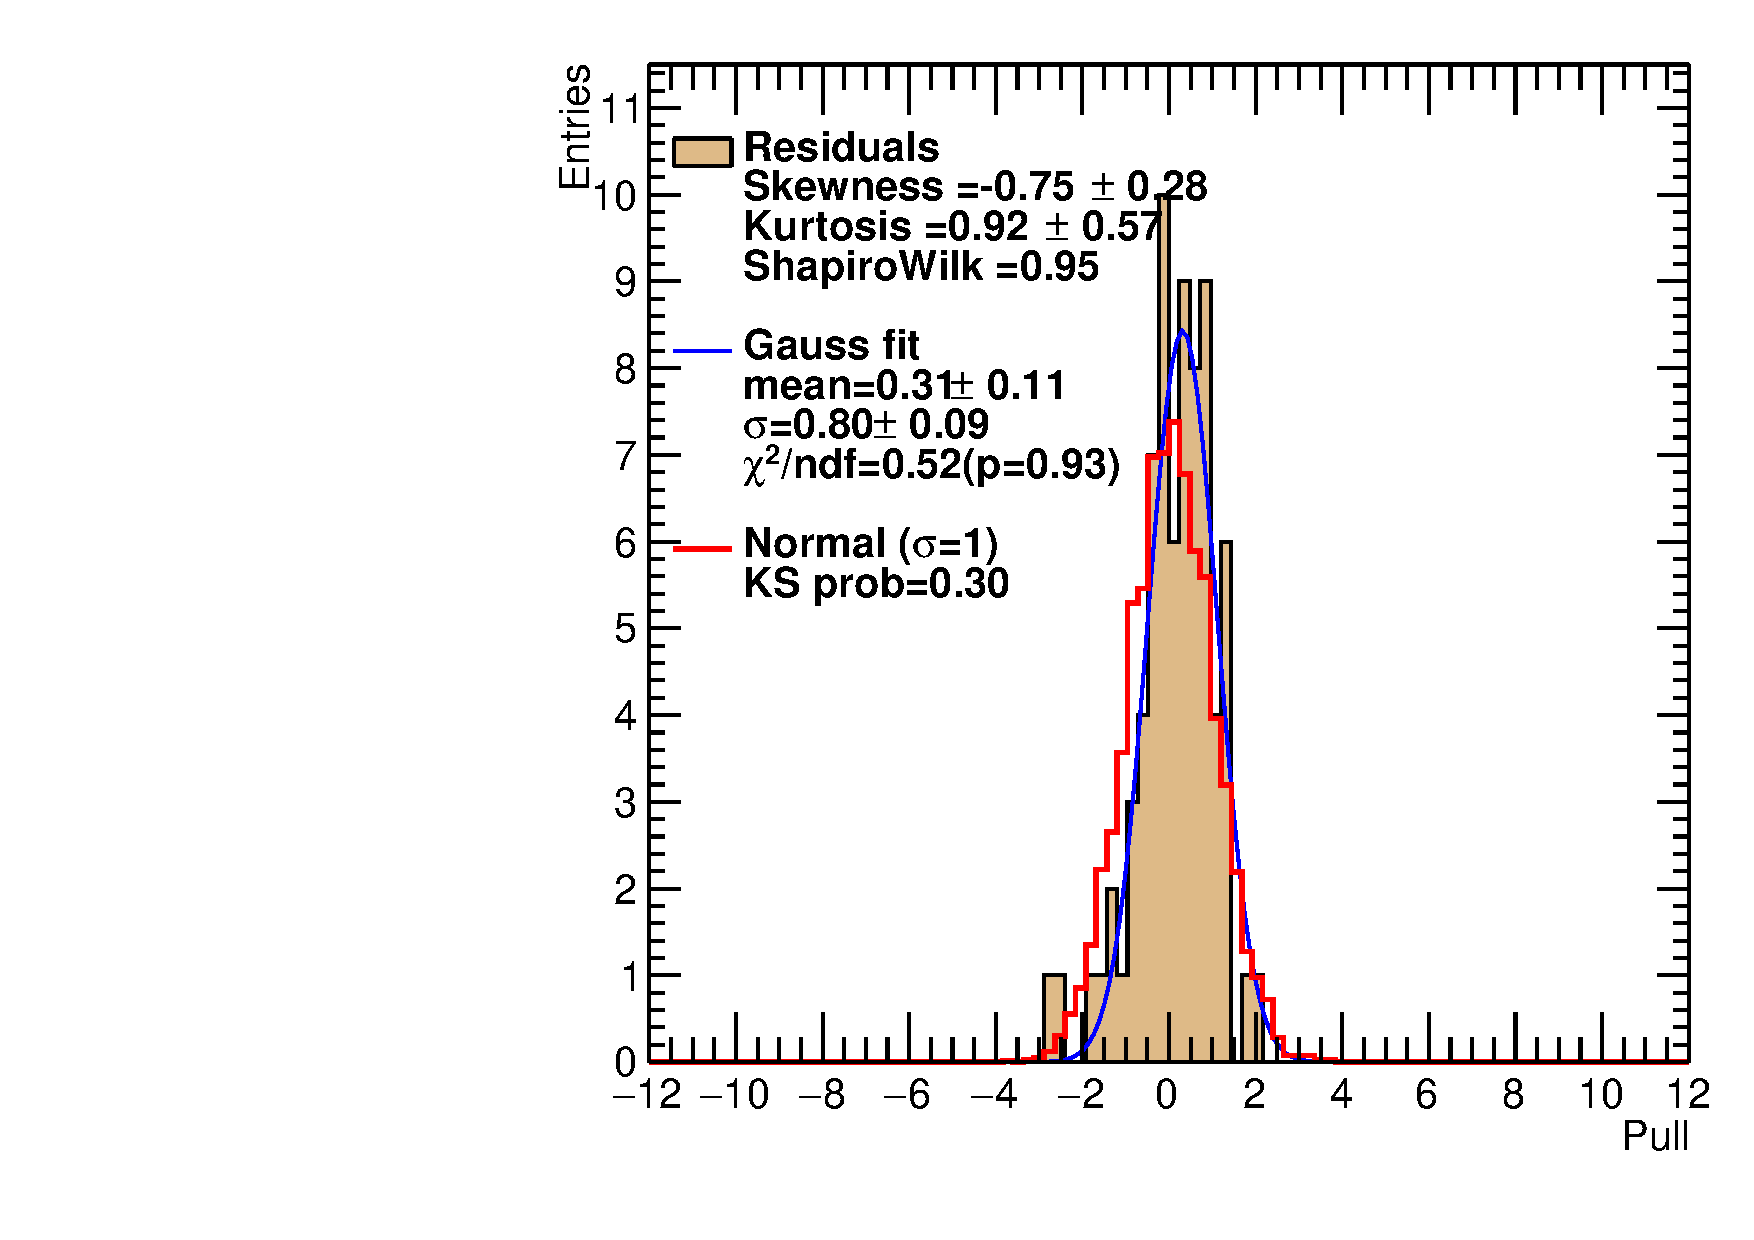
\includegraphics[scale=0.32]{figs/ch6/fit/variable_nosmooth/p5/10PB/pull_SMMCplusCR_Mbb_p5.pdf}%
    \caption{pulls of \mbb \ in p5}
    \end{subfigure}
    \hfill
    \begin{subfigure}[h]{0.38\linewidth}
    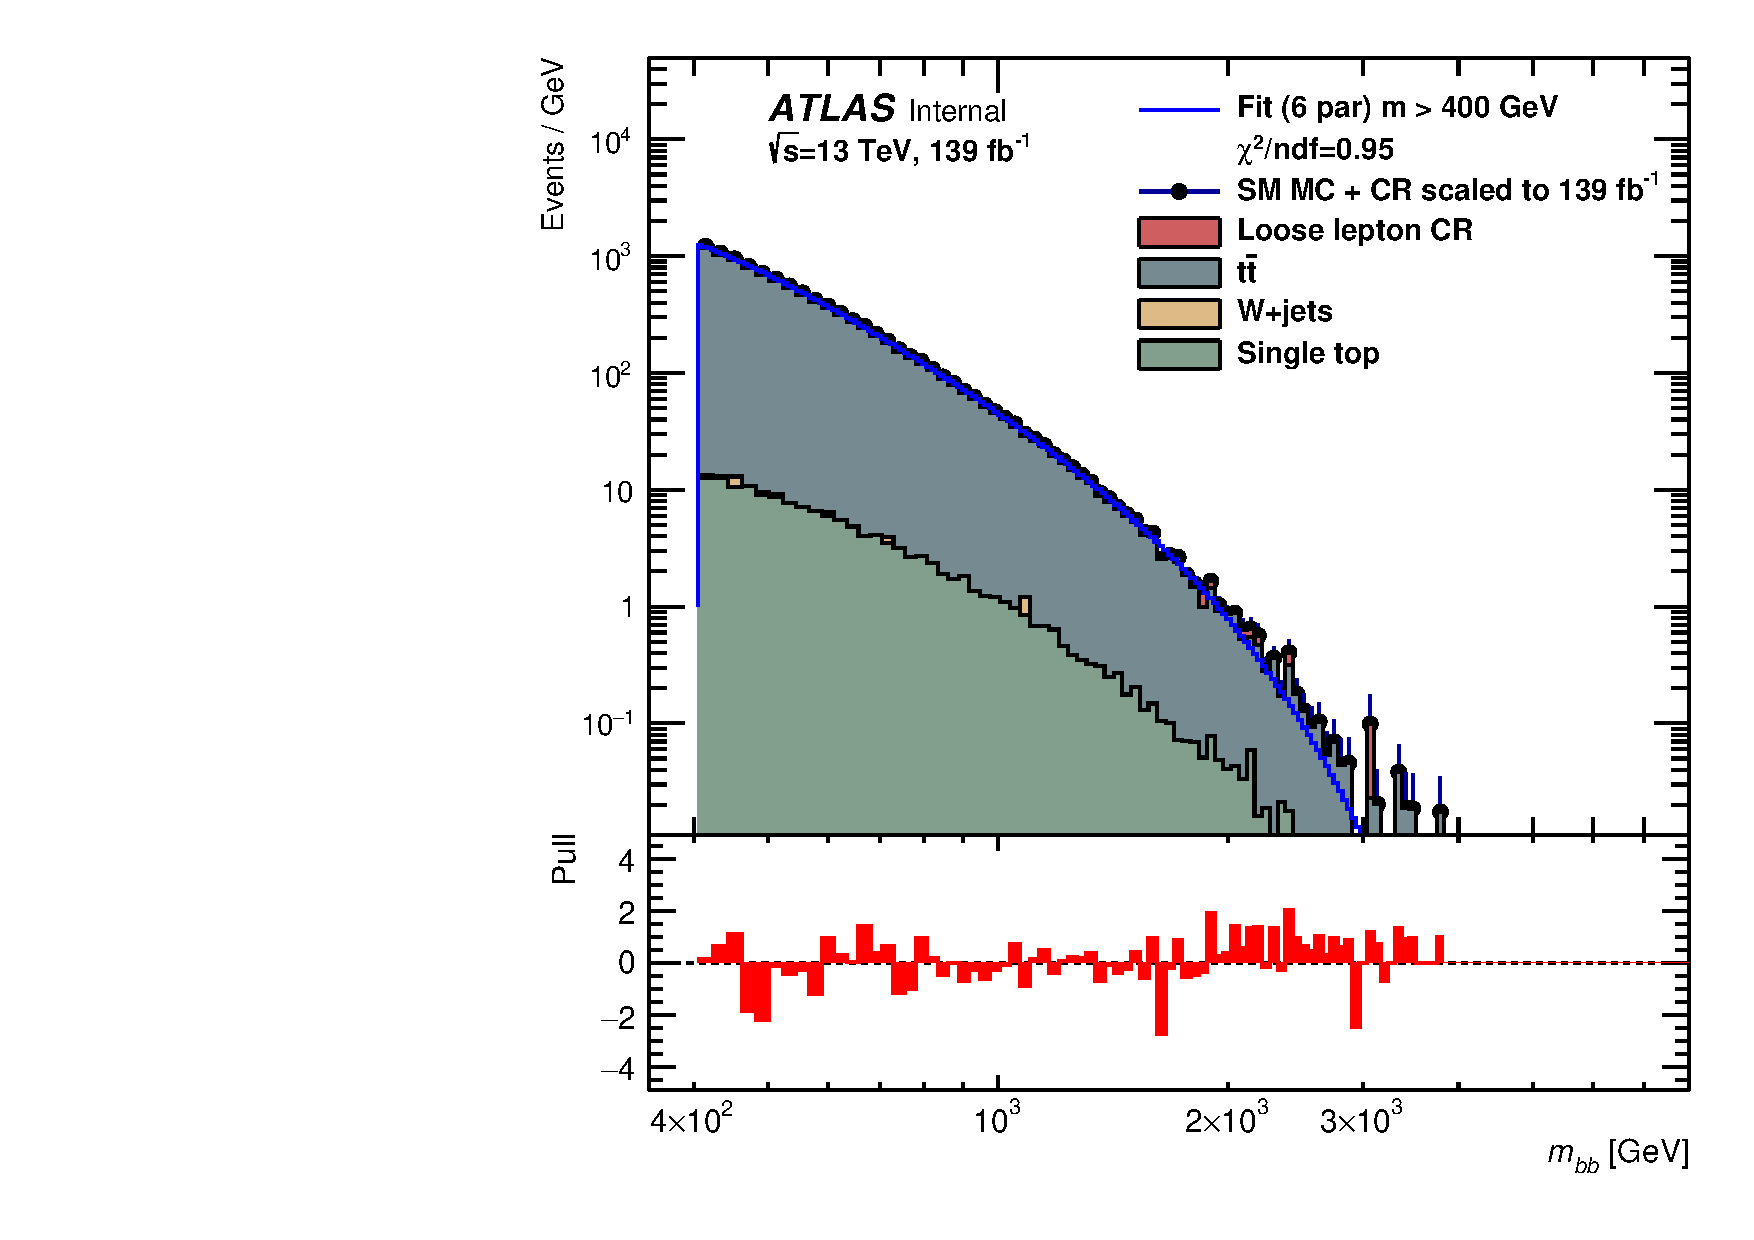
\includegraphics[scale=0.3]{figs/ch6/fit/variable_nosmooth/p6/10PB/output_SMMCplusCR_Mbb_p6.pdf}%
    \caption{\mbb \ using MC+LE-CR, p6}
    \end{subfigure}
    \hfill
    \begin{subfigure}[h]{0.4\linewidth}
    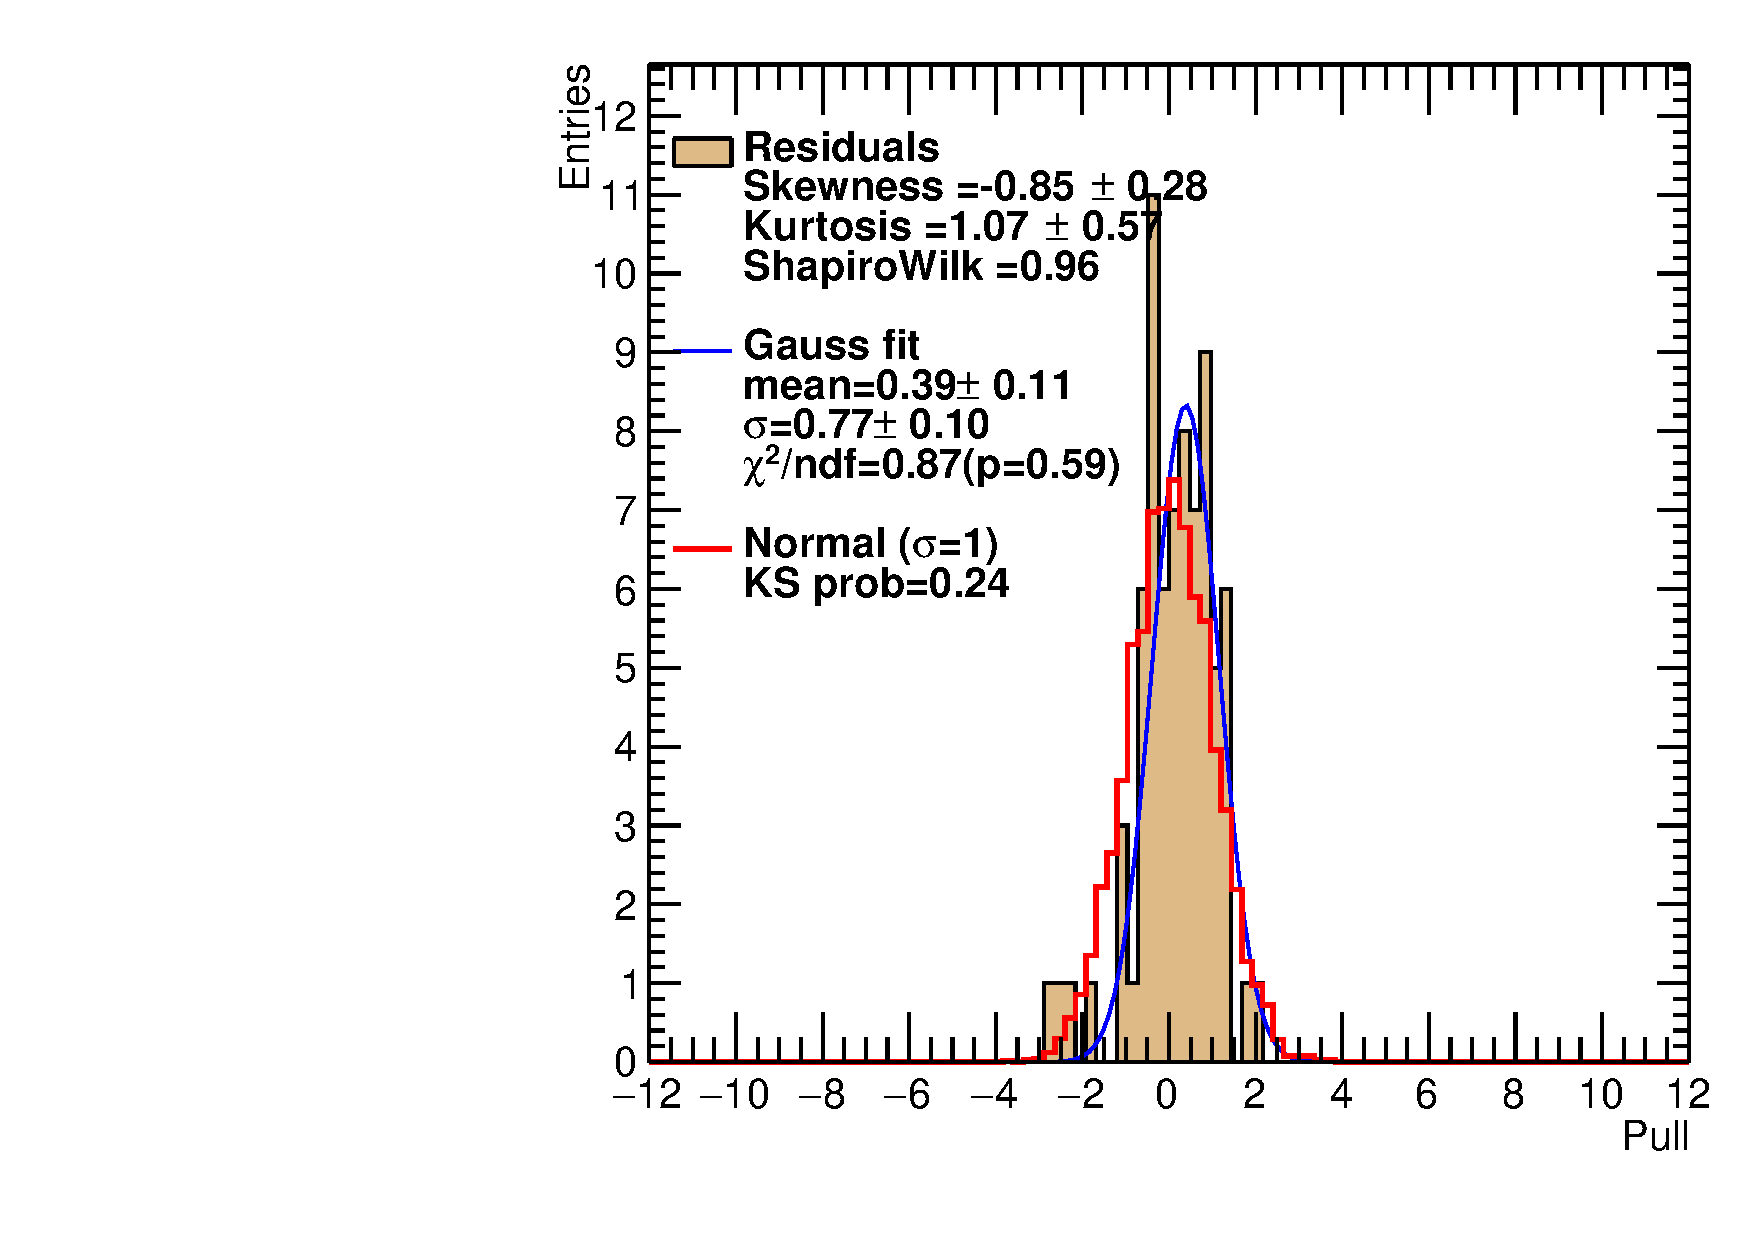
\includegraphics[scale=0.32]{figs/ch6/fit/variable_nosmooth/p6/10PB/pull_SMMCplusCR_Mbb_p6.pdf}%
    \caption{pulls of \mbb \ in p6}
    \end{subfigure}
    \hfill
    \caption{The \mbb \ invariant masses with the p4, p5 and p6 fit functions in the BSM region after the 10 pb AR cut is applied. Pulls shown on the right.}
\label{fig:mbb-fit-pulls}
\end{figure}

\newpage

\begin{figure}[H]
    \centering
    \begin{subfigure}[h]{0.38\linewidth}
    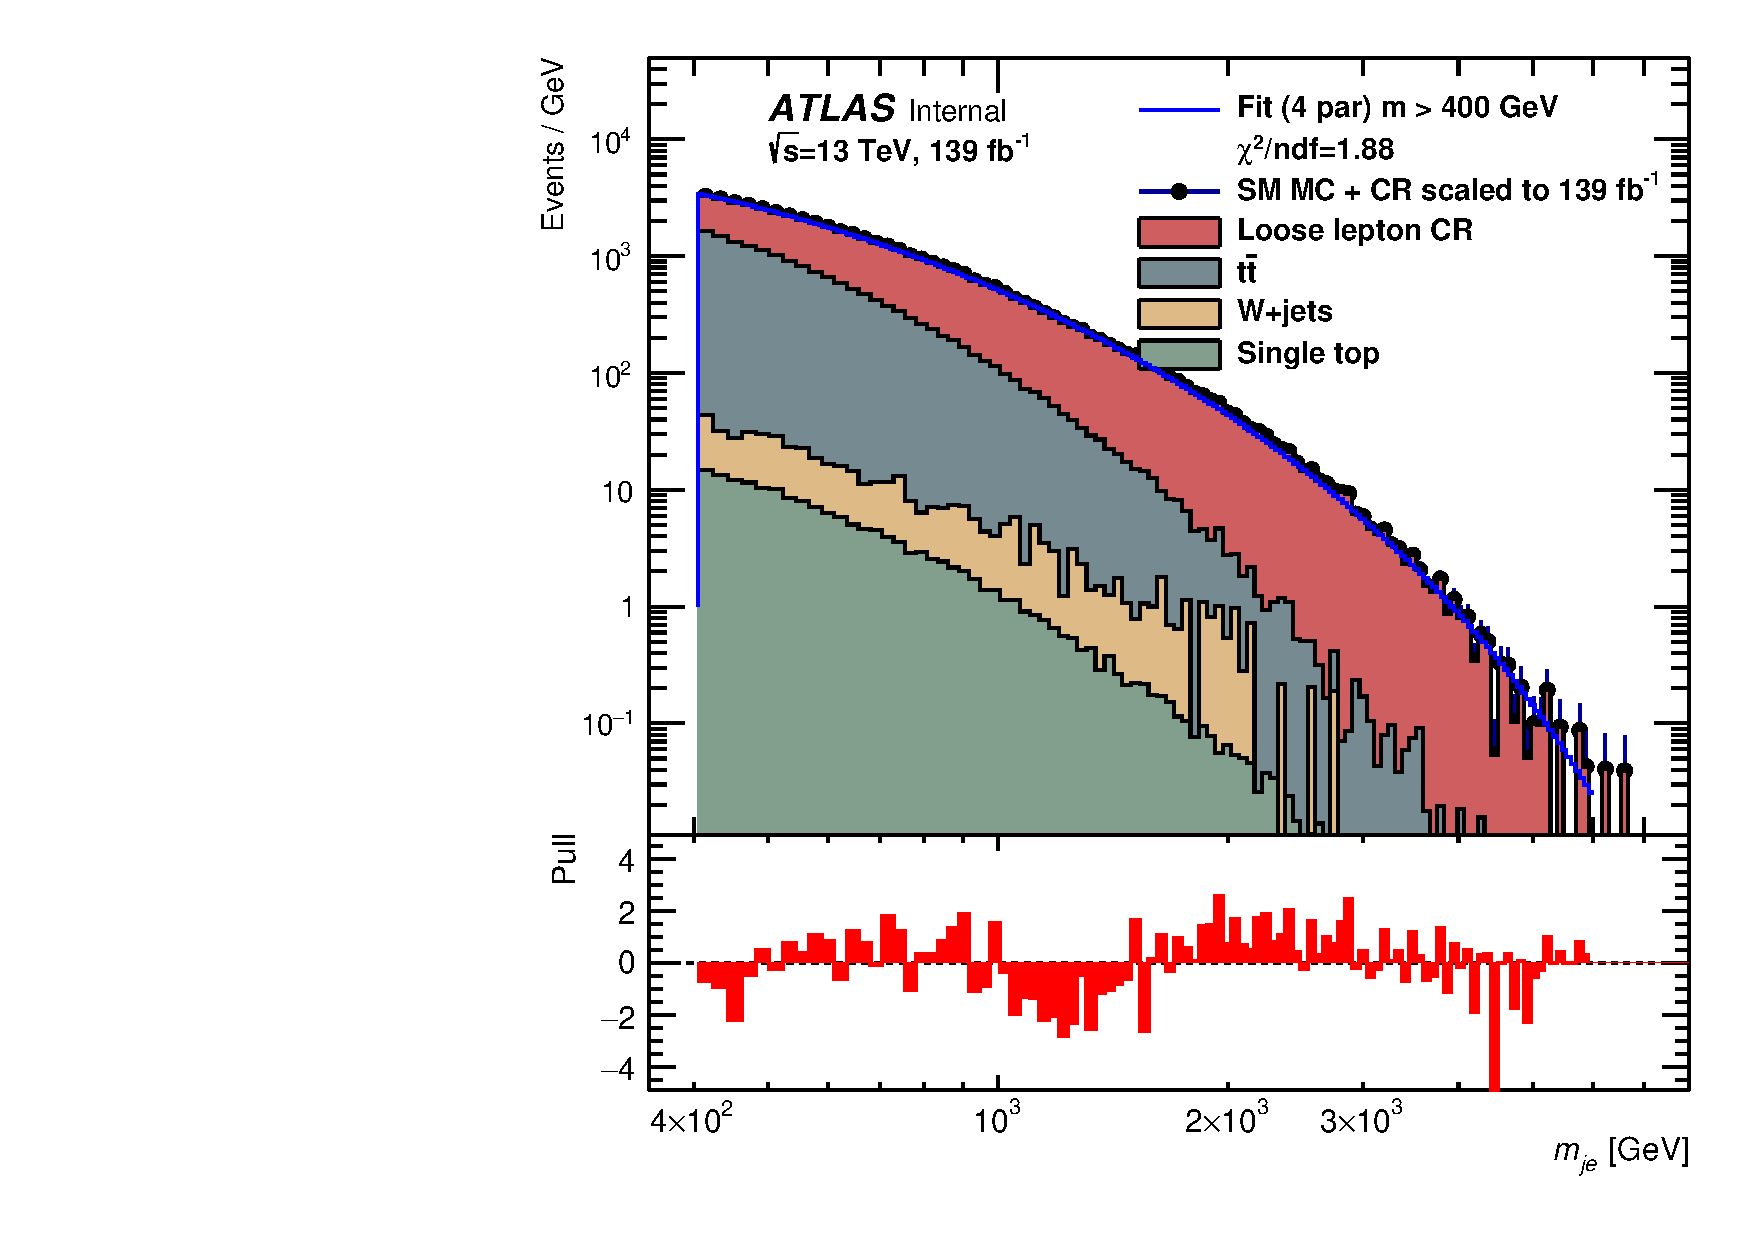
\includegraphics[scale=0.3]{figs/ch6/fit/variable_nosmooth/p4/10PB/output_SMMCplusCR_Mje_p4.pdf}%
    \caption{\mje \ using MC+LE-CR, p4}
    \end{subfigure}
    \hfill
    \begin{subfigure}[h]{0.4\linewidth}
    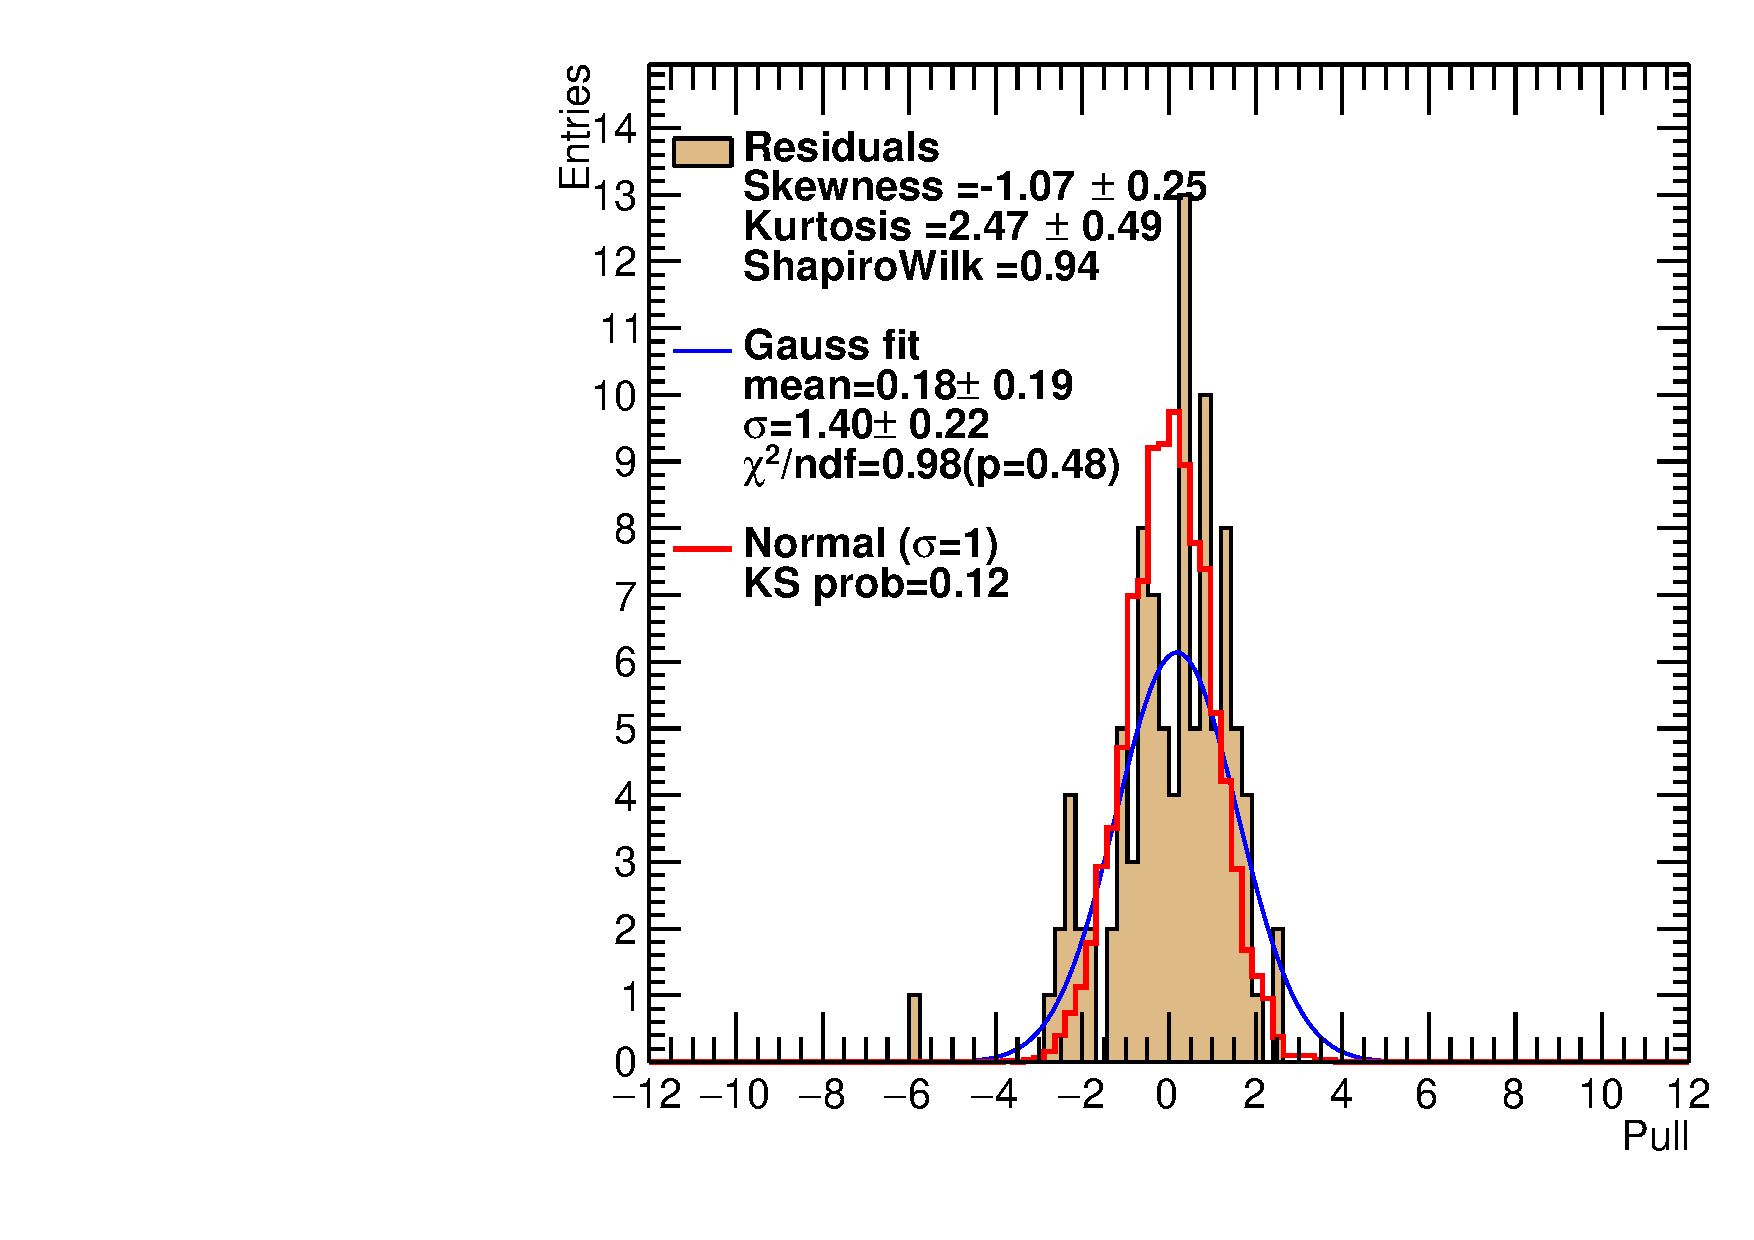
\includegraphics[scale=0.32]{figs/ch6/fit/variable_nosmooth/p4/10PB/pull_SMMCplusCR_Mje_p4.pdf}%
    \caption{pulls of \mje \ in p4}
    \end{subfigure}
    \hfill
    \begin{subfigure}[h]{0.38\linewidth}
    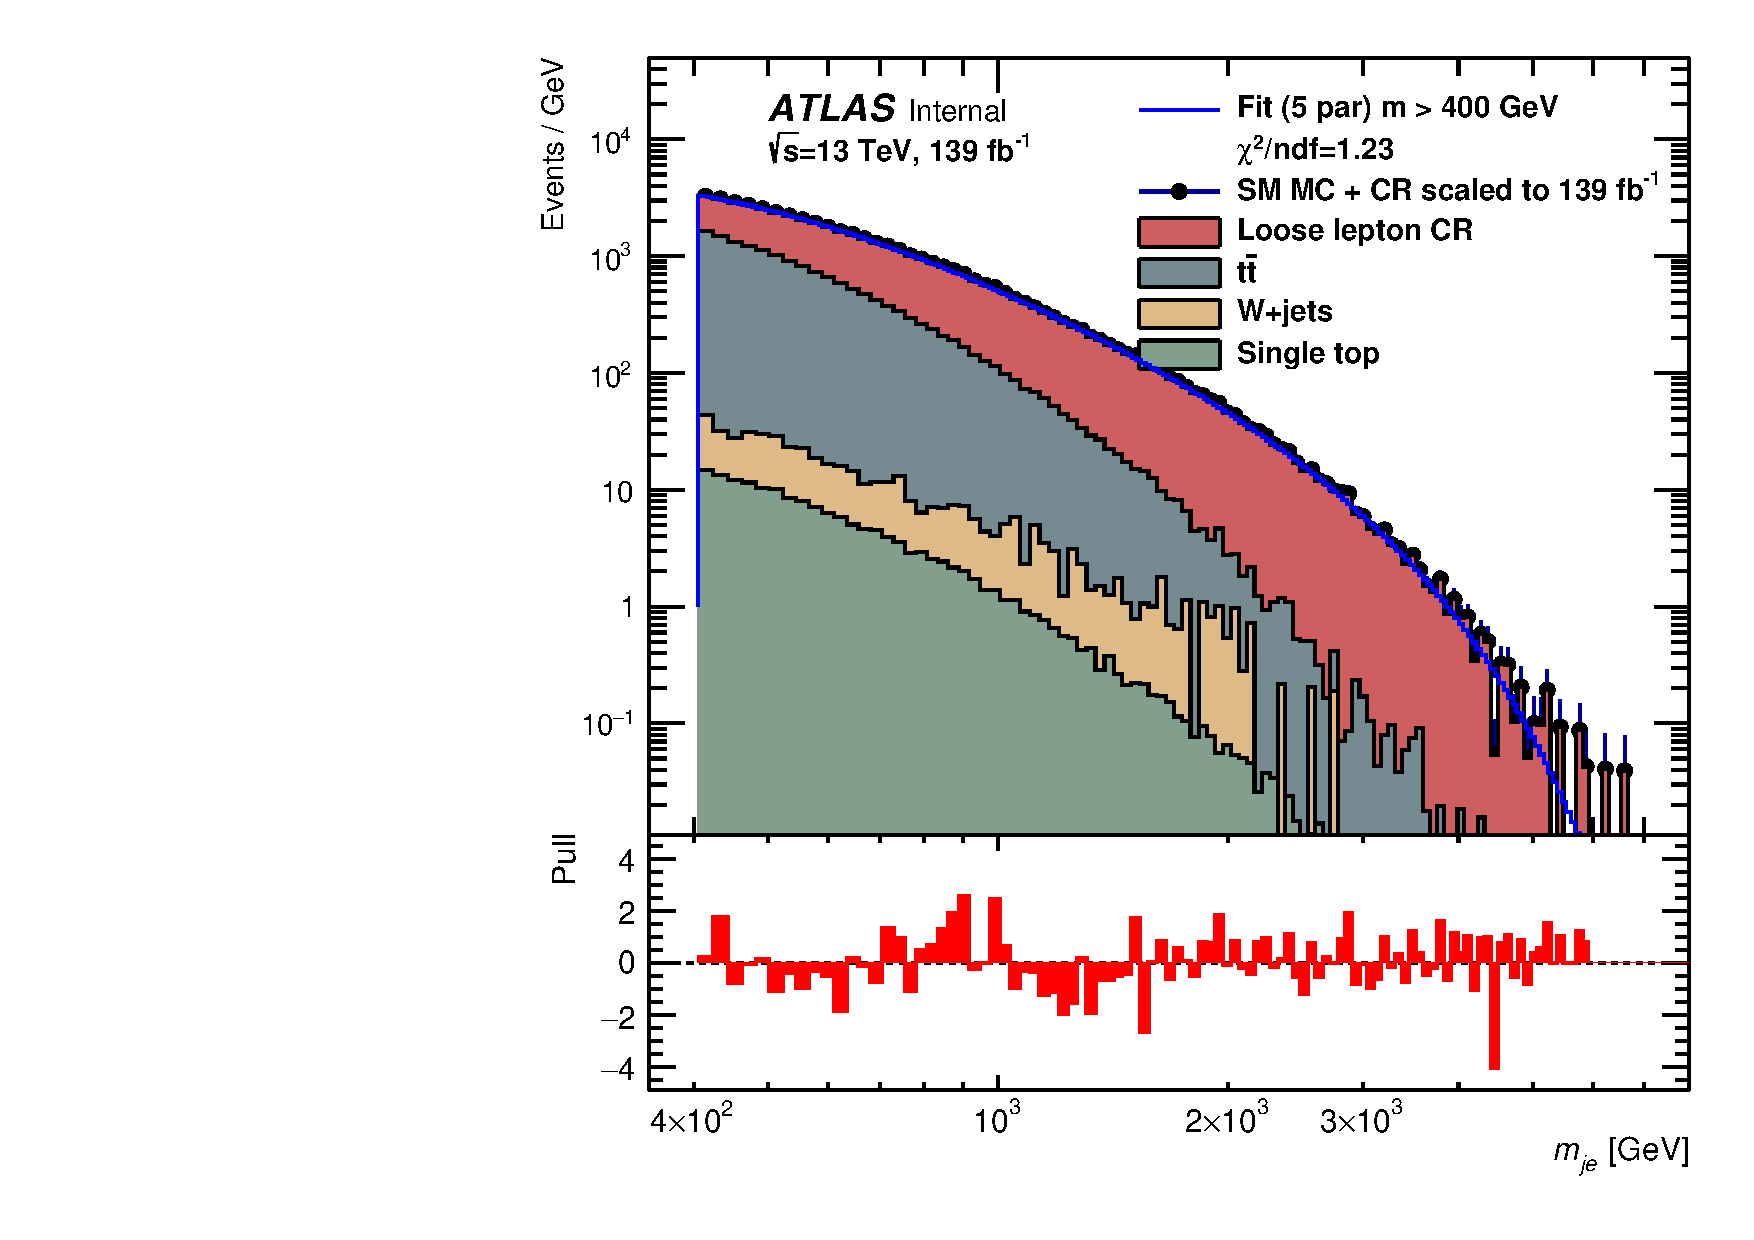
\includegraphics[scale=0.3]{figs/ch6/fit/variable_nosmooth/p5/10PB/output_SMMCplusCR_Mje_p5.pdf}%
     \caption{\mje \ using MC+LE-CR, p5}
     \end{subfigure}
     \hfill
    \begin{subfigure}[h]{0.4\linewidth}
    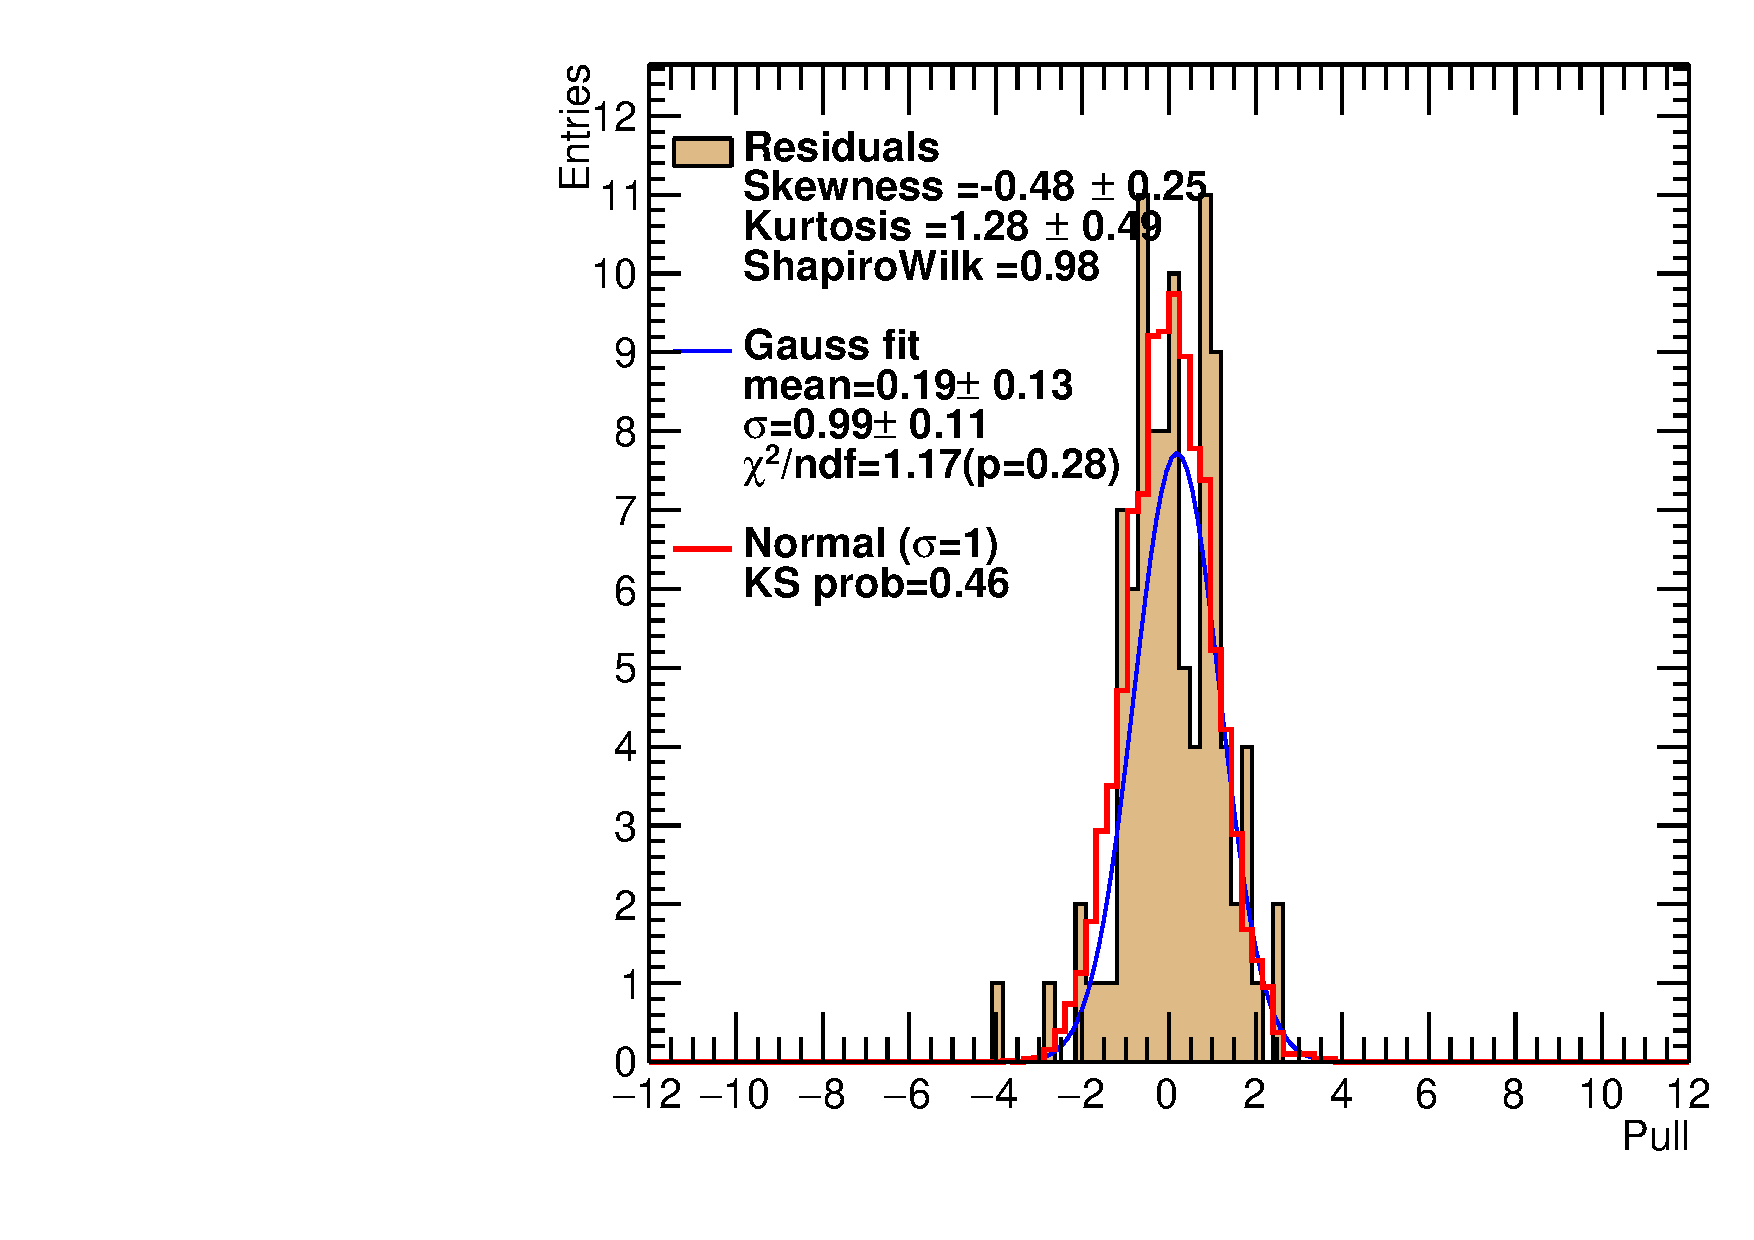
\includegraphics[scale=0.32]{figs/ch6/fit/variable_nosmooth/p5/10PB/pull_SMMCplusCR_Mje_p5.pdf}%
    \caption{pulls of \mje \ in p5}
    \end{subfigure}
    \hfill
    \begin{subfigure}[h]{0.38\linewidth}
    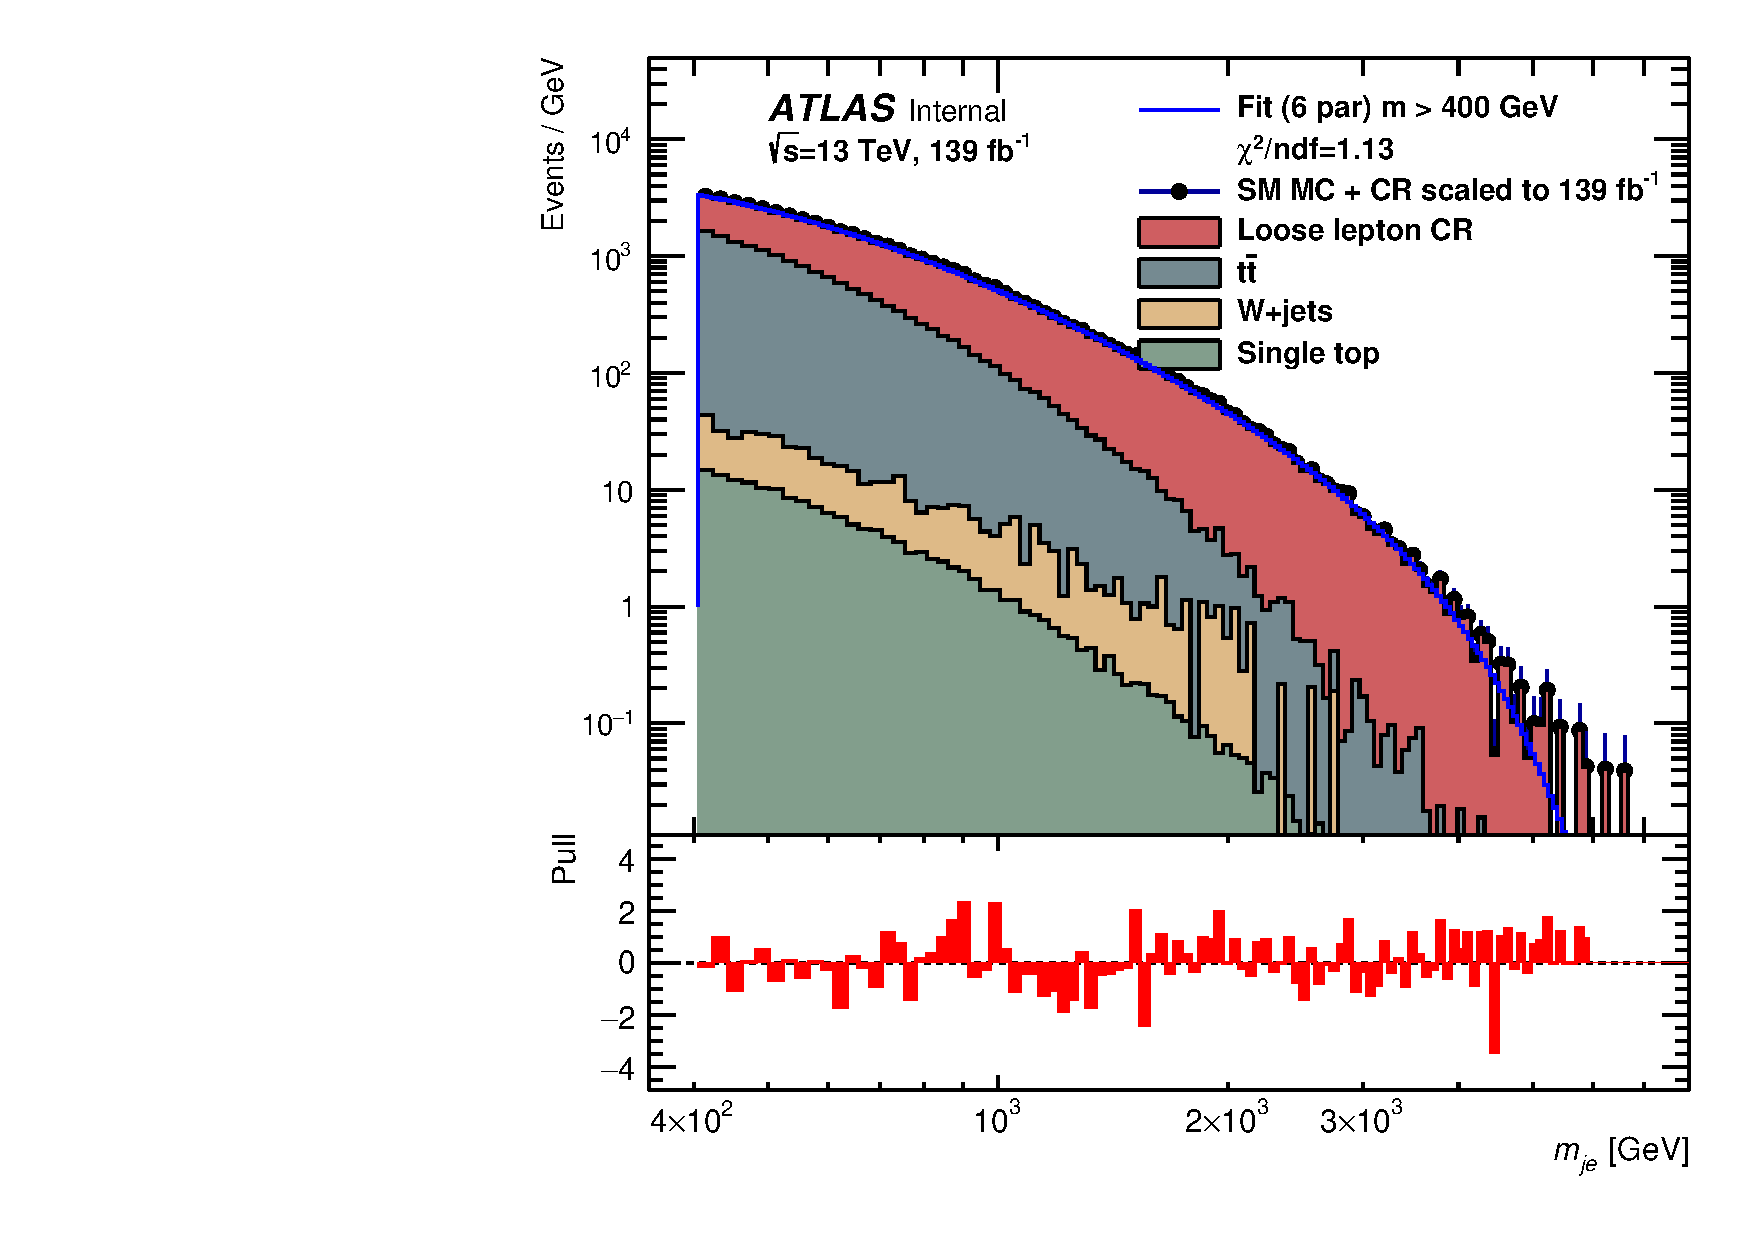
\includegraphics[scale=0.3]{figs/ch6/fit/variable_nosmooth/p6/10PB/output_SMMCplusCR_Mje_p6.pdf}%
    \caption{\mje \ using MC+LE-CR, p6}
    \end{subfigure}
    \hfill
    \begin{subfigure}[h]{0.4\linewidth}
    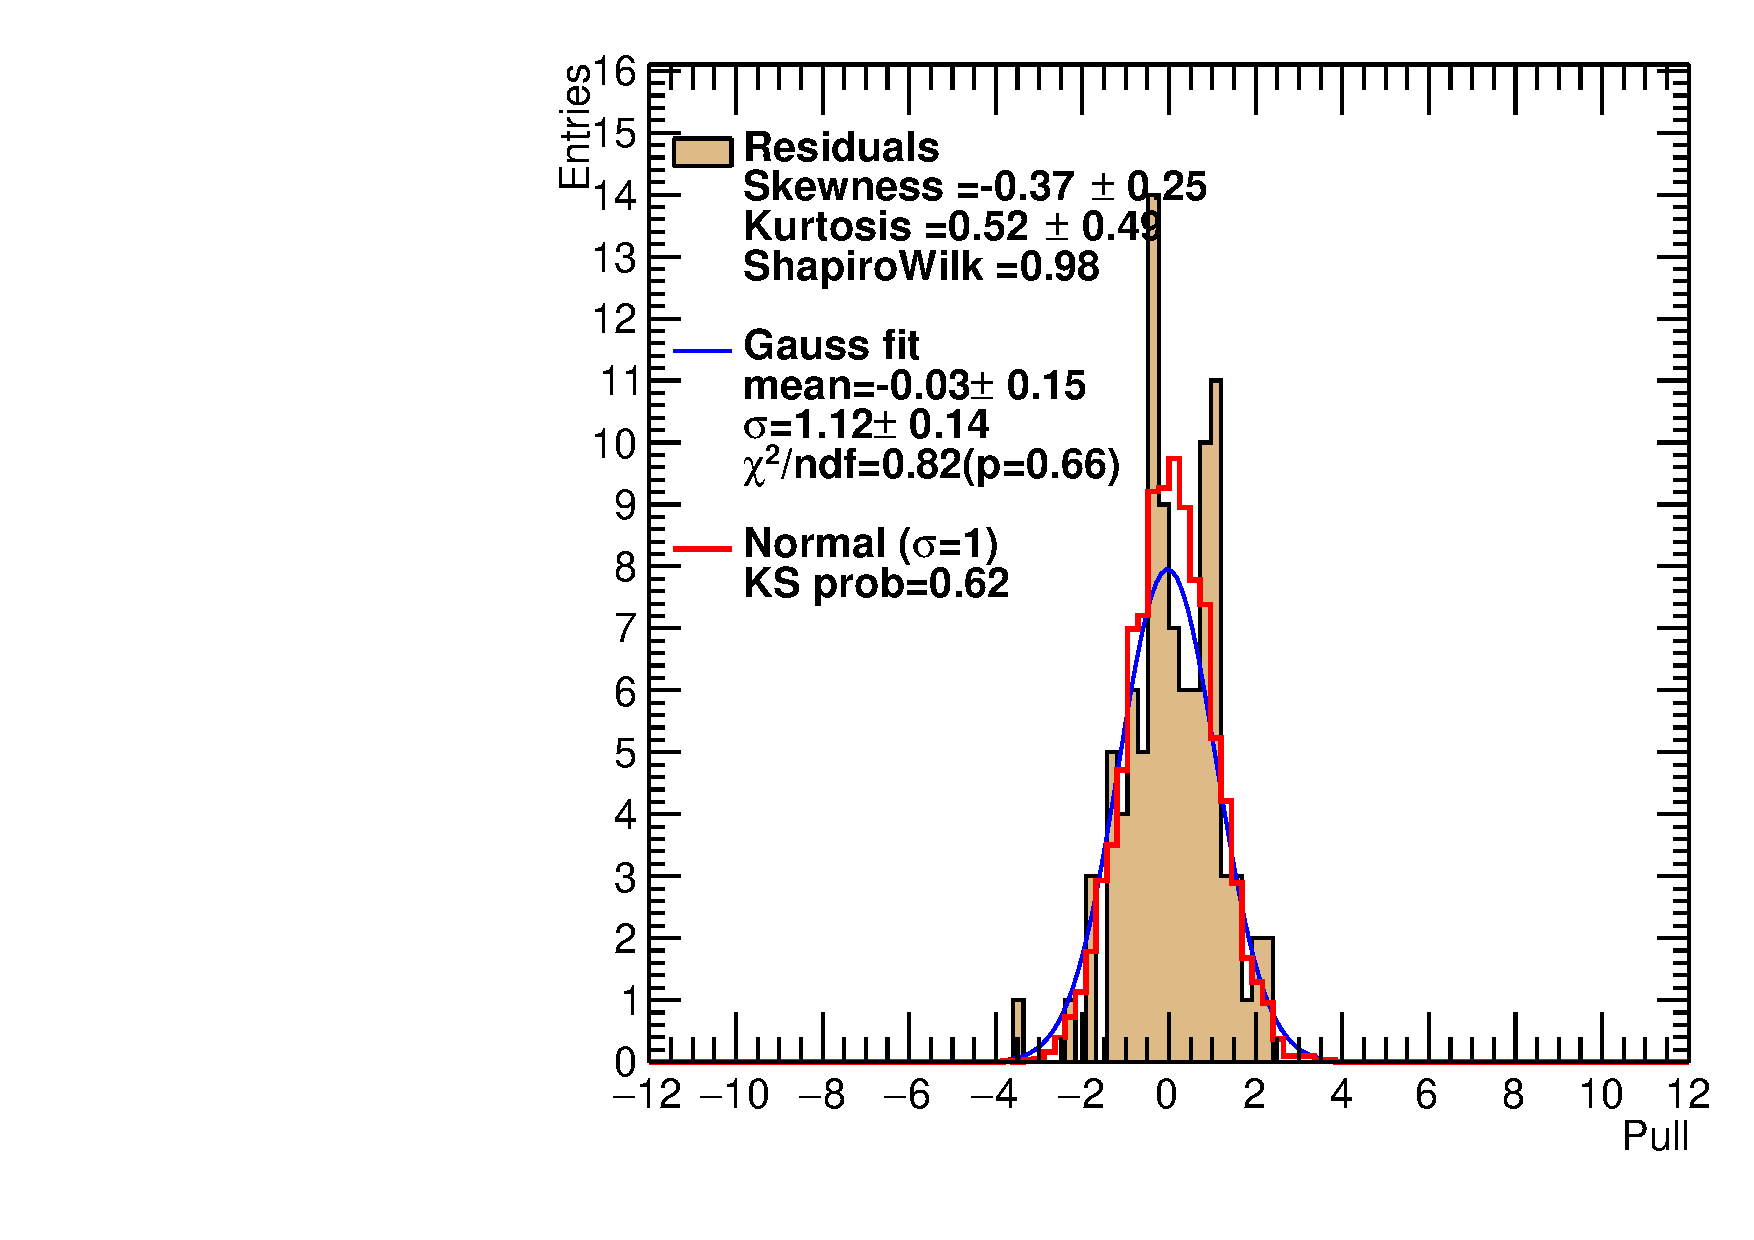
\includegraphics[scale=0.32]{figs/ch6/fit/variable_nosmooth/p6/10PB/pull_SMMCplusCR_Mje_p6.pdf}%
    \caption{pulls of \mje \ in p6}
    \end{subfigure}
    \hfill
    \caption{The \mje \ invariant masses with the p4, p5 and p6 fit functions in the BSM region after the 10 pb AR cut is applied. Pulls shown on the right.}
\label{fig:mje-fit-pulls}
\end{figure}

\begin{figure}[H]
    \centering
    \begin{subfigure}[h]{0.38\linewidth}
    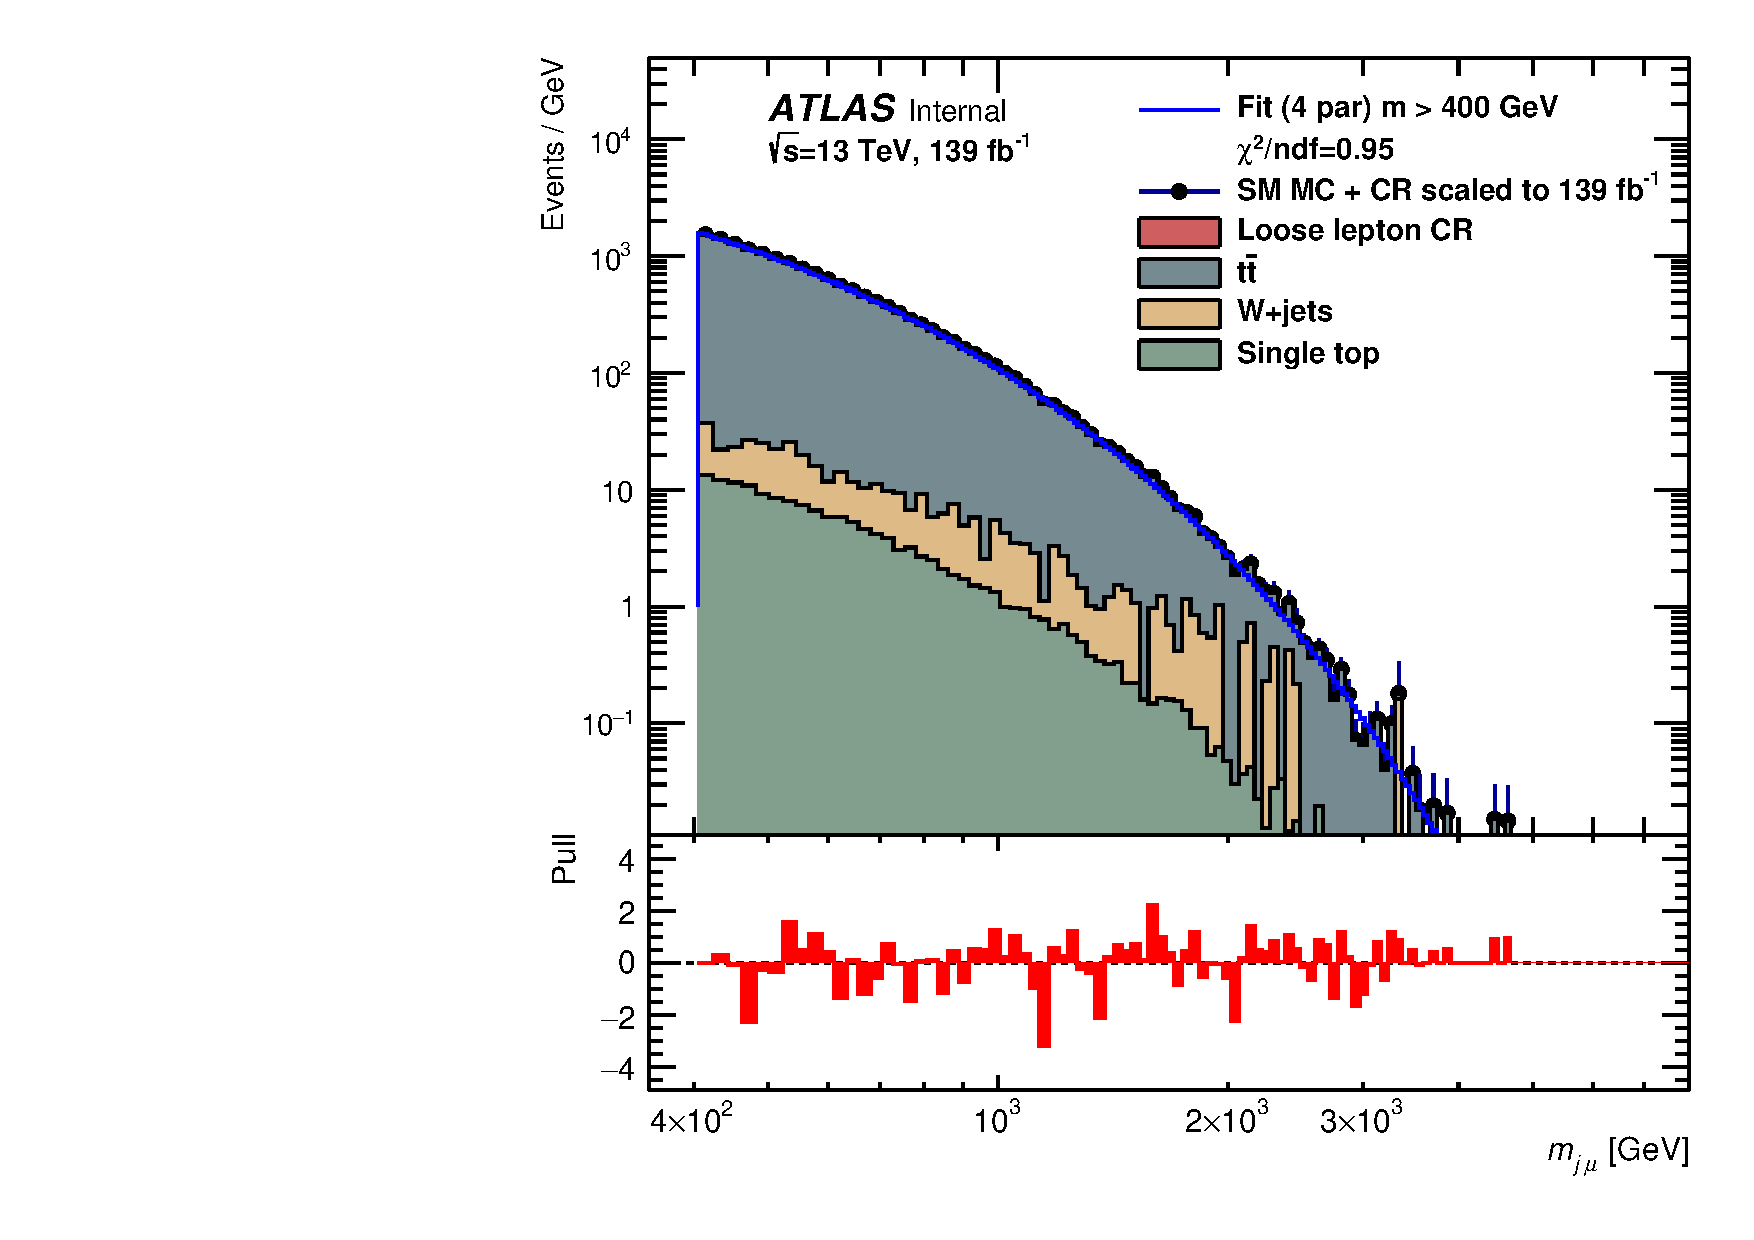
\includegraphics[scale=0.3]{figs/ch6/fit/variable_nosmooth/p4/10PB/output_SMMCplusCR_Mjm_p4.pdf}%
    \caption{\mjmu \ using MC+LE-CR, p4}
    \end{subfigure}
    \hfill
    \begin{subfigure}[h]{0.4\linewidth}
    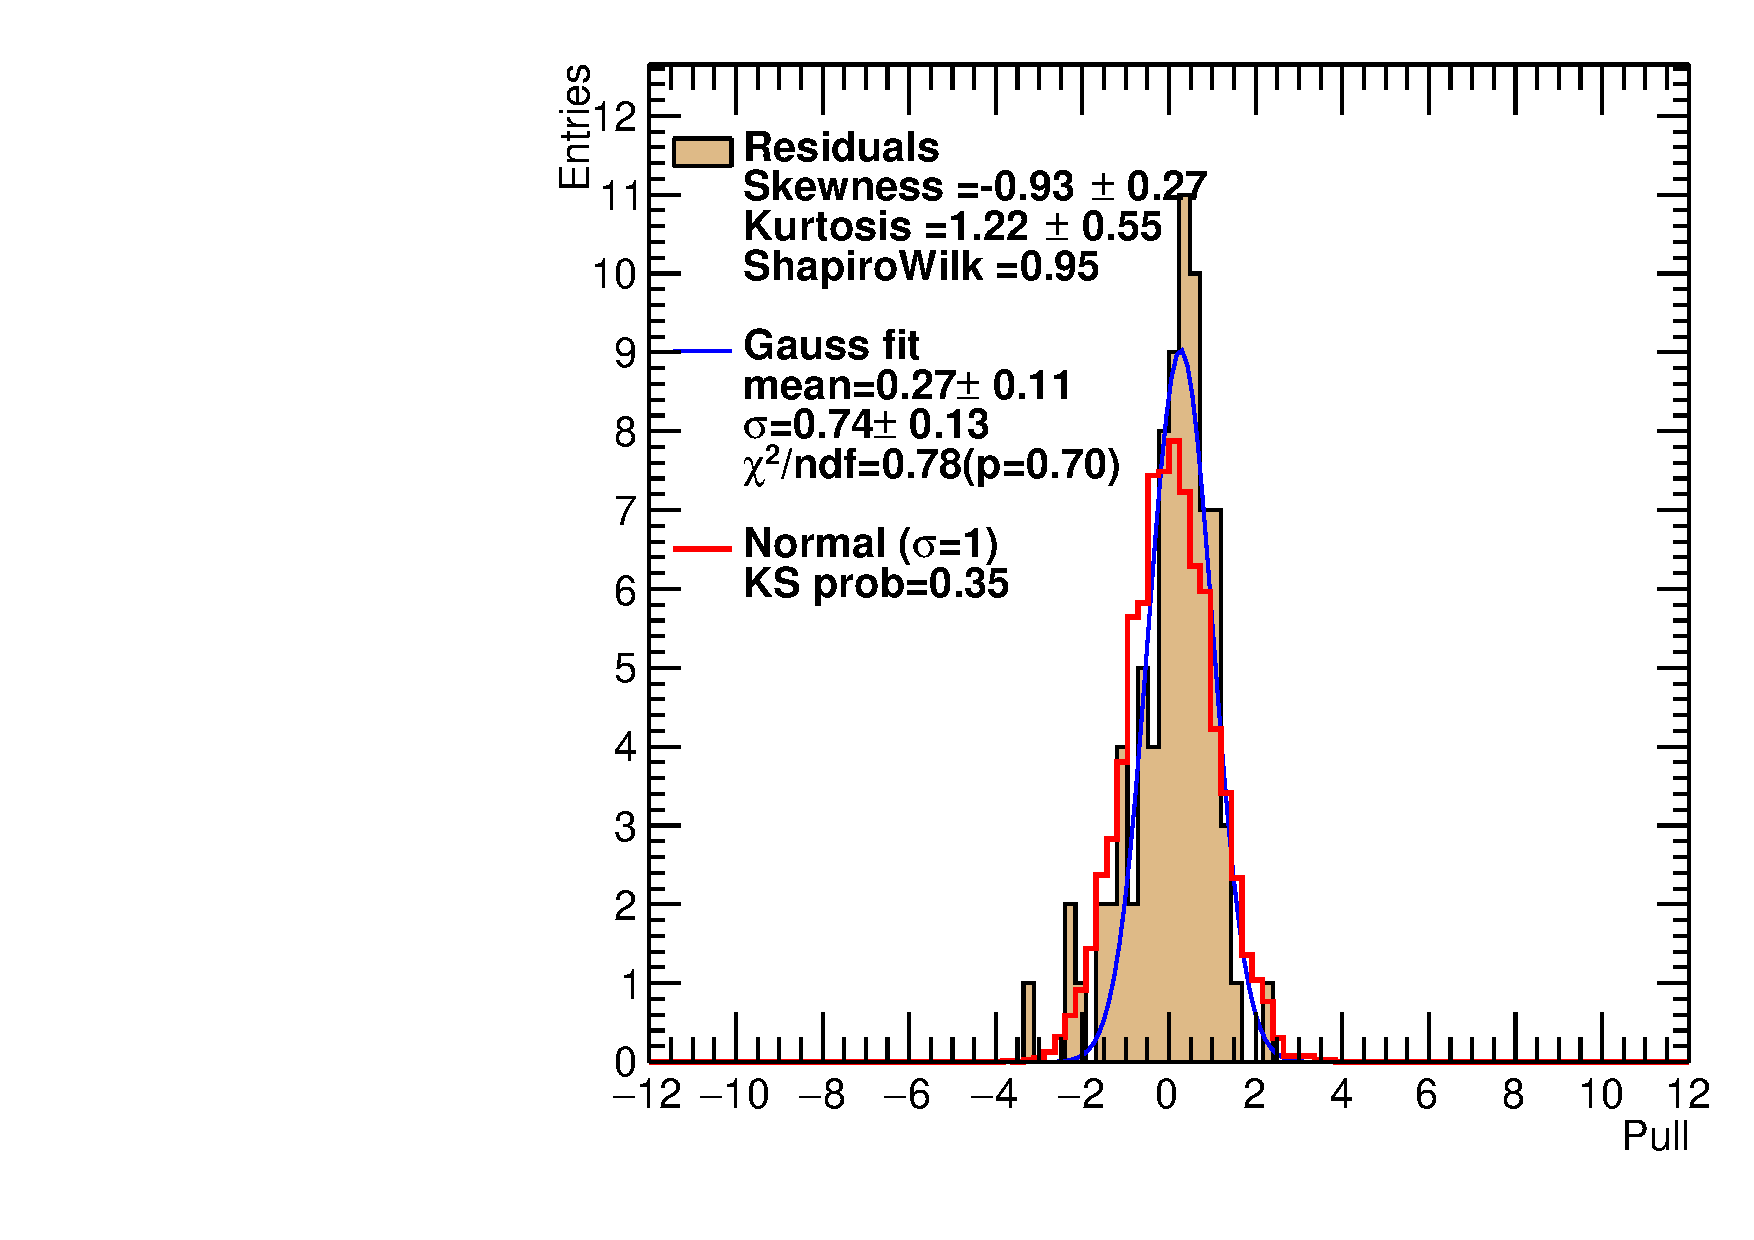
\includegraphics[scale=0.32]{figs/ch6/fit/variable_nosmooth/p4/10PB/pull_SMMCplusCR_Mjm_p4.pdf}%
    \caption{pulls of \mjmu \ in p4}
    \end{subfigure}
    \hfill
    \begin{subfigure}[h]{0.38\linewidth}
    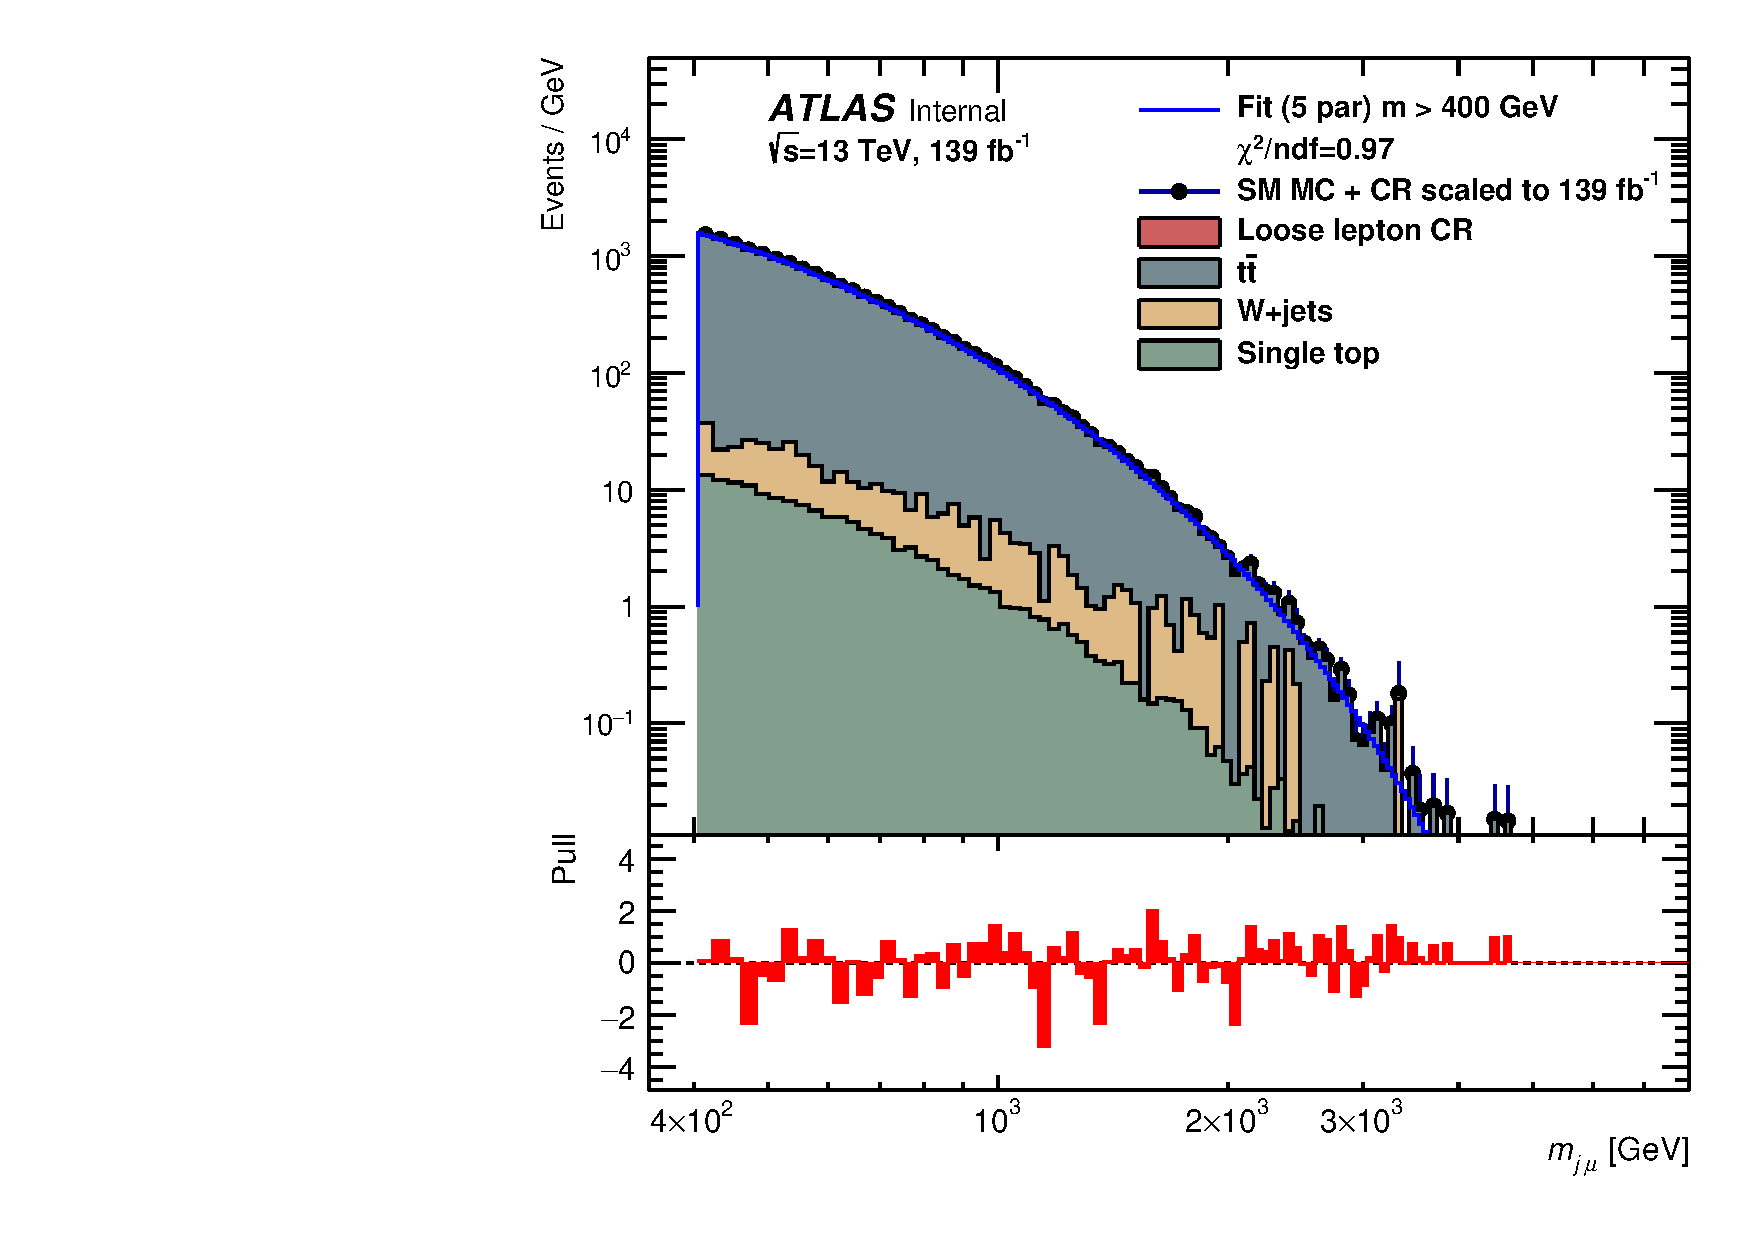
\includegraphics[scale=0.3]{figs/ch6/fit/variable_nosmooth/p5/10PB/output_SMMCplusCR_Mjm_p5.pdf}%
     \caption{\mjmu \ using MC+LE-CR, p5}
     \end{subfigure}
     \hfill
    \begin{subfigure}[h]{0.4\linewidth}
    \includegraphics[scale=0.32]{figs/ch6/fit/variable_nosmooth/p5/10PB/pull_SMMCplusCR_Mjm_p5.pdf}%
    \caption{pulls of \mjmu \ in p5}
    \end{subfigure}
    \hfill
    \begin{subfigure}[h]{0.38\linewidth}
    \includegraphics[scale=0.3]{figs/ch6/fit/variable_nosmooth/p6/10PB/output_SMMCplusCR_Mjm_p6.pdf}%
    \caption{\mjmu \ using MC+LE-CR, p6}
    \end{subfigure}
    \hfill
    \begin{subfigure}[h]{0.4\linewidth}
    \includegraphics[scale=0.32]{figs/ch6/fit/variable_nosmooth/p6/10PB/pull_SMMCplusCR_Mjm_p6.pdf}%
    \caption{pulls of \mjmu \ in p6}
    \end{subfigure}
    \hfill
    \caption{The \mjmu \ invariant masses with the p4, p5 and p6 fit functions in the BSM region after the 10 pb AR cut is applied. Pulls shown on the right.}
\label{fig:mjm-fit-pulls}
\end{figure}

\newpage

\begin{figure}[H]
    \centering
    \begin{subfigure}[h]{0.38\linewidth}
    \includegraphics[scale=0.3]{figs/ch6/fit/variable_nosmooth/p4/10PB/output_SMMCplusCR_Mjg_p4.pdf}%
    \caption{\mjph \ using MC+LE-CR, p4}
    \end{subfigure}
    \hfill
    \begin{subfigure}[h]{0.4\linewidth}
    \includegraphics[scale=0.32]{figs/ch6/fit/variable_nosmooth/p4/10PB/pull_SMMCplusCR_Mjg_p4.pdf}%
    \caption{pulls of \mjph \ in p4}
    \end{subfigure}
    \hfill
    \begin{subfigure}[h]{0.38\linewidth}
    \includegraphics[scale=0.3]{figs/ch6/fit/variable_nosmooth/p5/10PB/output_SMMCplusCR_Mjg_p5.pdf}%
     \caption{\mjph \ using MC+LE-CR, p5}
     \end{subfigure}
     \hfill
    \begin{subfigure}[h]{0.4\linewidth}
    \includegraphics[scale=0.32]{figs/ch6/fit/variable_nosmooth/p5/10PB/pull_SMMCplusCR_Mjg_p5.pdf}%
    \caption{pulls of \mjph \ in p5}
    \end{subfigure}
    \hfill
    \begin{subfigure}[h]{0.38\linewidth}
    \includegraphics[scale=0.3]{figs/ch6/fit/variable_nosmooth/p6/10PB/output_SMMCplusCR_Mjg_p6.pdf}%
    \caption{\mjph \ using MC+LE-CR, p6}
    \end{subfigure}
    \hfill
    \begin{subfigure}[h]{0.4\linewidth}
    \includegraphics[scale=0.32]{figs/ch6/fit/variable_nosmooth/p6/10PB/pull_SMMCplusCR_Mjg_p6.pdf}%
    \caption{pulls of \mjph \ in p6}
    \end{subfigure}
    \hfill
    \caption{The \mjph \ invariant masses with the p4, p5 and p6 fit functions in the BSM region after the 10 pb AR cut is applied. Pulls shown on the right.}
\label{fig:mjg-fit-pulls}
\end{figure}

\newpage


\begin{figure}[H]
    \centering
    \begin{subfigure}[h]{0.38\linewidth}
    \includegraphics[scale=0.3]{figs/ch6/fit/variable_nosmooth/p4/10PB/output_SMMCplusCR_Mbe_p4.pdf}%
    \caption{\mbe \ using MC+LE-CR, p4}
    \end{subfigure}
    \hfill
    \begin{subfigure}[h]{0.4\linewidth}
    \includegraphics[scale=0.32]{figs/ch6/fit/variable_nosmooth/p4/10PB/pull_SMMCplusCR_Mbe_p4.pdf}%
    \caption{pulls of \mbe \ in p4}
    \end{subfigure}
    \hfill
    \begin{subfigure}[h]{0.38\linewidth}
    \includegraphics[scale=0.3]{figs/ch6/fit/variable_nosmooth/p5/10PB/output_SMMCplusCR_Mbe_p5.pdf}%
     \caption{\mbe \ using MC+LE-CR, p5}
     \end{subfigure}
     \hfill
    \begin{subfigure}[h]{0.4\linewidth}
    \includegraphics[scale=0.32]{figs/ch6/fit/variable_nosmooth/p5/10PB/pull_SMMCplusCR_Mbe_p5.pdf}%
    \caption{pulls of \mbe \ in p5}
    \end{subfigure}
    \hfill
    \begin{subfigure}[h]{0.38\linewidth}
    \includegraphics[scale=0.3]{figs/ch6/fit/variable_nosmooth/p6/10PB/output_SMMCplusCR_Mbe_p6.pdf}%
    \caption{\mbe \ using MC+LE-CR, p6}
    \end{subfigure}
    \hfill
    \begin{subfigure}[h]{0.4\linewidth}
    \includegraphics[scale=0.32]{figs/ch6/fit/variable_nosmooth/p6/10PB/pull_SMMCplusCR_Mbe_p6.pdf}%
    \caption{pulls of \mbe \ in p6}
    \end{subfigure}
    \hfill
    \caption{The \mbe \ invariant masses with the p4, p5 and p6 fit functions in the BSM region after the 10 pb AR cut is applied. Pulls shown on the right.}
\label{fig:mbe-fit-pulls}
\end{figure}

\newpage


\begin{figure}[H]
    \centering
    \begin{subfigure}[h]{0.38\linewidth}
    \includegraphics[scale=0.3]{figs/ch6/fit/variable_nosmooth/p4/10PB/output_SMMCplusCR_Mbm_p4.pdf}%
    \caption{\mbmu \ using MC+LE-CR, p4}
    \end{subfigure}
    \hfill
    \begin{subfigure}[h]{0.4\linewidth}
    \includegraphics[scale=0.32]{figs/ch6/fit/variable_nosmooth/p4/10PB/pull_SMMCplusCR_Mbm_p4.pdf}%
    \caption{pulls of \mbmu \ in p4}
    \end{subfigure}
    \hfill
    \begin{subfigure}[h]{0.38\linewidth}
    \includegraphics[scale=0.3]{figs/ch6/fit/variable_nosmooth/p5/10PB/output_SMMCplusCR_Mbm_p5.pdf}%
     \caption{\mbmu \ using MC+LE-CR, p5}
     \end{subfigure}
     \hfill
    \begin{subfigure}[h]{0.4\linewidth}
    \includegraphics[scale=0.32]{figs/ch6/fit/variable_nosmooth/p5/10PB/pull_SMMCplusCR_Mbm_p5.pdf}%
    \caption{pulls of \mbmu \ in p5}
    \end{subfigure}
    \hfill
    \begin{subfigure}[h]{0.38\linewidth}
    \includegraphics[scale=0.3]{figs/ch6/fit/variable_nosmooth/p6/10PB/output_SMMCplusCR_Mbm_p6.pdf}%
    \caption{\mbmu \ using MC+LE-CR, p6}
    \end{subfigure}
    \hfill
    \begin{subfigure}[h]{0.4\linewidth}
    \includegraphics[scale=0.32]{figs/ch6/fit/variable_nosmooth/p6/10PB/pull_SMMCplusCR_Mbm_p6.pdf}%
    \caption{pulls of \mbmu \ in p6}
    \end{subfigure}
    \hfill
    \caption{The \mbmu \ invariant masses with the p4, p5 and p6 fit functions in the BSM region after the 10 pb AR cut is applied. Pulls shown on the right.}
\label{fig:mbm-fit-pulls}
\end{figure}

\newpage


\begin{figure}[H]
    \centering
    \begin{subfigure}[h]{0.38\linewidth}
    \includegraphics[scale=0.3]{figs/ch6/fit/variable_nosmooth/p4/10PB/output_SMMCplusCR_Mbg_p4.pdf}%
    \caption{\mbph \ using MC+LE-CR, p4}
    \end{subfigure}
    \hfill
    \begin{subfigure}[h]{0.4\linewidth}
    \includegraphics[scale=0.32]{figs/ch6/fit/variable_nosmooth/p4/10PB/pull_SMMCplusCR_Mbg_p4.pdf}%
    \caption{pulls of \mbph \ in p4}
    \end{subfigure}
    \hfill
    \begin{subfigure}[h]{0.38\linewidth}
    \includegraphics[scale=0.3]{figs/ch6/fit/variable_nosmooth/p5/10PB/output_SMMCplusCR_Mbg_p5.pdf}%
     \caption{\mbph \ using MC+LE-CR, p5}
     \end{subfigure}
     \hfill
    \begin{subfigure}[h]{0.4\linewidth}
    \includegraphics[scale=0.32]{figs/ch6/fit/variable_nosmooth/p5/10PB/pull_SMMCplusCR_Mbg_p5.pdf}%
    \caption{pulls of \mbph \ in p5}
    \end{subfigure}
    \hfill
    \begin{subfigure}[h]{0.38\linewidth}
    \includegraphics[scale=0.3]{figs/ch6/fit/variable_nosmooth/p6/10PB/output_SMMCplusCR_Mbg_p6.pdf}%
    \caption{\mbph \ using MC+LE-CR, p6}
    \end{subfigure}
    \hfill
    \begin{subfigure}[h]{0.4\linewidth}
    \includegraphics[scale=0.32]{figs/ch6/fit/variable_nosmooth/p6/10PB/pull_SMMCplusCR_Mbg_p6.pdf}%
    \caption{pulls of \mbph \ in p6}
    \end{subfigure}
    \hfill
    \caption{The \mbph \ invariant masses with the p4, p5 and p6 fit functions in the BSM region after the 10 pb AR cut is applied. Pulls shown on the right.}
\label{fig:mbg-fit-pulls}
\end{figure}

\newpage

The p4 fit shows several failures in the statistical tests. However, the p5 fit function shows good agreement for most of the invariant masses, though there 
are a few that should be pointed out. 

\begin{itemize}
    \item \mbb - Failed 4 tests (mean, sigma, skewness, kurtosis) while the other three tests are good. This is due to problems in \gls{mc} background that use the \gls{le-cr}.
    Though, this region shows good agreement with the p5 function when using stage-1 10\% unblinded data as seen in Appendix \ref{appendix:10data-fit-studies} (only fails two tests).
    \item \mjmu - Failed 4 tests (mean, KS, skewness, kurtosis), while the other three are good. This is mainly because the \gls{le-cr} does not contribute to the μ-channel, 
    essentially the fit is only applied to the MC simulations. The stage-1 10\% unblinded data in Appendix \ref{appendix:10data-fit-studies} passes all test but one. 
\end{itemize}

\newpage

\section{Results}

Now that the \gls{ar}s are defined and a reasonable, well tested fit function has been selected to describe the background hypothesis, results can be obtained by unblinding 
100\% of the Run 2 data to see if any anomalous resonant signatures are found using the \gls{bh} strategy. Figure~\ref{fig:loss-full-data} shows two plots using the full 100\% unblinded Run 2 data 
along with the five \gls{bsm} models (Figure\ref{fig:bsm-loss} shows the analogous 10\% of data with scaling). 

\begin{figure}[ht]
    \centering
    \begin{subfigure}[h]{0.4\linewidth}
    \includegraphics[scale=0.35]{figs/ch6/results/pub_loss_cut_all_sum_run2.pdf}%
    \caption{}
    \end{subfigure}
    \hfill
    \begin{subfigure}[h]{0.4\linewidth}
    \includegraphics[scale=0.35]{figs/ch6/results/pub_loss_cut_all_sum_run3.pdf}%
    \caption{}
    \end{subfigure}
    \hfill
    \caption{Distributions of anomaly scores in data and the five benchmark BSM models. (a) shows these BSM models each at the 2 TeV mass hypotheses scaled to the expected events 
    for 140 $\textrm{fb}^{\textrm{-1}}$. (b) shows these five BSM models at the 6 TeV mass hypothesis also scaled to the expected events 
    for 140 $\textrm{fb}^{\textrm{-1}}$. The vertical red lines on both show the three defined ARs.}
\label{fig:loss-full-data}
\end{figure}

Figure~\ref{fig:results-data-before} shows the results of the likelihood fit on 100\% unblinded Run 2 data for each of the nine invariant masses of interest. This figure is \textbf{before} any of 
the three \gls{ar} cuts are applied. The largest deviation found using the \gls{bh} strategy is in the \mjmu channel in the mass range of 0.44-0.48 TeV. The 
global \textit{p}-value is 0.057 which corresponds to Z = 1.5$\sigma$. The local significance of this mass range is found to be \textit{p}-value = 0.00022, corresponding to 
Z = 3.5$\sigma$. The yellow bands show the fit uncertainty ($\pm\sigma$). Figure~\ref{fig:results-data-after} shows the BumpHunter results for the fully unblinded Run 2 data within the 10 pb gls{ar}. 
\newpage

\begin{figure}[H]
    \centering
    \includegraphics[scale=0.8]{figs/ch6/results/pub_mass_BH_before_yellow.pdf}%
\caption{BumpHunter results for full unblinded Run 2 data for all nine invariant masses of interest before applying any of the three AR cuts. It also shows the result of the 
5p fit function to describe the background hypothesis. The lower panel shows the bin-by-bin fit significances with the largest deviation reported by BumpHunter noted by the 
vertical dashed lines with its global p-value shown.}
\label{fig:results-data-before}
\end{figure}

\newpage

\begin{figure}[H]
    \centering
    \includegraphics[scale=0.8]{figs/ch6/results/pub_mass_BH_10pb_yellow.pdf}%
\caption{BumpHunter results for full unblinded Run 2 data for all nine invariant masses of interest after applying the 10 pb AR cut. It also shows the result of the 
5p fit function to describe the background hypothesis. The lower panel shows the bin-by-bin fit significances with the largest deviation reported by BumpHunter noted by the 
vertical dashed lines with its global p-value shown.}
\label{fig:results-data-after}
\end{figure}

\newpage

The largest deviation that's worth discussing can be found in Figure~\ref{fig:results-data-after} in the \mjmu distribution on the bottom right. This deviance is found near 
the mass point 4.6-4.8 TeV. This has a local \textit{p}-value of 3.8$\times\textrm{10}^{\textrm{-5}}$ corresponding to a significance of Z = 3.9$\sigma$. Accounting for the 
look-elsewhere effect for the \mjmu distribution, the global \textit{p}-value is 0.013, corresponding to a global significance of Z = 2.2$\sigma$
\par
The metric of discovery sensitivity \cite{disc-sens} is briefly discussed in the Appendix~\ref{appendix:sb-improvements} and is defined in Eq.~\ref{eq:app:1.1}. This value
was calculated for each \gls{bsm} model and all their mass hypothesis. These values are and plotted in Figure~\ref{fig:results-data-sig} in the bin that's associated to its mass. This figure shows 
the increase of discovery sensitivity after the 10 pb \gls{ar} cut is applied. Some increases are as large as 200\% for some models. Some models, such as \gls{ssm}, show 
little (if any) improvement. This is due (in case of \gls{ssm}) to the fact that the signatures of these models are nearly identical to the \gls{sm} background. The two plots
that involve a photon (\mjph and \mbph) show almost no increase nor decrease. This is because none of the chosen \gls{bsm} benchmark models require a photon in the final state. 
There is also a noticeable trend that the discovery sensitivity generally increases as the mass hypotheses of these \gls{bsm} models increase. This makes sense since high mass 
particles tend to decay into more anomalous events and therefore will pass the \gls{ar} cuts. 

\begin{figure}[H]
    \centering
    \includegraphics[scale=0.8]{figs/ch6/results/pub_mass_BSM_significance_run.pdf}%
\caption{Bin-by-bin improvement in ΔZ discovery sensitivity after applying the 10 pb AR cut for all nine invariant masses of interest.
         Discovery sensitivity increases shown for all five benchmark BSM models and all their mass hypothesis.}
\label{fig:results-data-sig}
\end{figure}

\subsection{Limit Setting}

Most analyses are non-generic and have a specific \gls{bsm} model with a range of possible heavy masses that are studied. Limits are then able to be set on these masses generated 
from the model of interest once the background hypotheses is used to find deviations. This analysis is unique in the case that it is a generic search and only used \gls{bsm} models 
for benchmark metrics. It was decided in the end to set limits using Gaussian shapes placed at a large range of possible mass hypotheses. 
\par
The limits found in this analysis uses the frequentist method that is based on a profile likelihood ratio between the fit function, the estimated background, and the possible 
signature. In the case of upper limits, the statistical model $\textrm{\textit{f}}(\textrm{\textit{data}}|\textrm{μ},\alpha)$, where μ is the parameter representing a 
signal yield and $\alpha$ are the nuisance parameters. The profile likelihood from the fit function is used to generate different statistics to test alternative signal+background 
and background hypotheses. To reduce sensitivity, the confidence level (\gls{cl}) procedure adds an additional test statistic $\bar{q}_{\mu}$ used for upper limits~\cite{limit-setting}.
The \textit{p}-values for the μ(s+b) and μ=0 (background only) hypotheses are analyzed by a large ensemble of pseudo-experiments.
\par
The mean signal Gaussian shapes implemented for limit setting are defined as a hypothetical mass and have values in GeV at:

\begin{itemize}
    \item 300, 320, 340, 360, 380,
    \item 500, 530, 560, 590,
    \item 400, 420, 440, 460, 480,
    \item 620, 650, 680,
    \item 710, 750, 790,
    \item 830, 870,
    \item 910, 960,
    \item 1000, 1100, 1200, 1300, 1400, 1500, 1600, 1700, 1800, 1900,
    \item 2000, 2100, 2200, 2300, 2400, 2500, 2600, 2700, 2800, 2900,
    \item 3000, 3200, 3400, 3600, 3800,
    \item 4000, 4200, 4400, 4600, 4800,
    \item 5000, 5300, 5600, 5900,
    \item 6200, 6500, 6800,
    \item 7100, 7500, 7900
\end{itemize}

The \gls{cl} level was set to 95\% for the observe upper limits on the $\sigma \times BR \times Acc  \times  Eff$ for Gaussian shaped signal with various widths
are seen in Figure~\ref{fig:freq-limit}.

\newpage

\begin{figure}[H]
    \centering
    \includegraphics[scale=0.7]{figs/ch6/results/merge_gaus.pdf}%
\caption{The 95\% CL observed upper limits on cross-section times acceptance (A), efficiency ($\epsilon$) and branching ratio (B) for Gaussian signal shapes with various widths.
         Limits are calculated on events within the 10 pb AR. The $\pm \textrm{1}\sigma$ and $\pm \textrm{2}\sigma$ bands are shown for $\sigma_{\textrm{X}}/\textrm{m}_{\textrm{X}}$=0}
\label{fig:freq-limit}
\end{figure}
